% !TEX TS-program = xelatex
% !BIB program = biber
% !TEX encoding = UTF-8 Unicode

% --------------------------------------------------
% Token-level Genomic Foundation Model Fine-tuning
% for Metagenomic Taxonomic Classification
% National Taiwan University - Master's Thesis
% --------------------------------------------------

\documentclass[
    ncsstyle  = false,
    watermark = false,
    doi       = false,
    doctype   = draft,
    print     = false,
    removetemp = false,
]{ncs-thesis}

% To speed up building, comment out chapters you don't need
\includeonly{
    front/acknowledgement,
    front/abstract,
    front/denotation,
    contents/chapter01,
    contents/chapter02,
    contents/chapter03,
    contents/chapter04,
    contents/chapter05,
    back/appendix01,
}

% Uncomment to include all chapters:
% \includeonly{}

\addbibresource{./back/references.bib}
% !TeX root = ./main.tex

% --------------------------------------------------
% 資訊設定（Information Configs）
% --------------------------------------------------

\ntusetup{
  university*   = {National Taiwan University},
  university    = {國立臺灣大學},
  college       = {電機資訊學院},
  college*      = {College of Electrical Engineering and Computer Science},
  institute     = {生醫電子與資訊學研究所},
  institute*    = {Institute of Biomedical Electronics and Informatics},
  title         = {基於基因體基礎模型之總體基因體短讀序列分類學分類},
  title*        = {Token-level Genomic Foundation Model Fine-tuning \\ for Metagenomic Taxonomic Classification},
  author        = {楊明儒},
  author*       = {Ming-Ju Yang},
  ID            = {R13945009},
  advisor       = {劉子毓},
  advisor*      = {Tzu-Yu Liu},
  date          = {2026-07-01},
  oral-date     = {2026-07-01},
  DOI           = {},
  keywords      = {基因體基礎模型, 總體基因體學, 分類學分類, 低秩適應, 注意力池化},
  keywords*     = {Genomic Foundation Model, Metagenomics, Taxonomic Classification, LoRA, Attention Pooling},
}

% --------------------------------------------------
% 加載套件（Include Packages）
% --------------------------------------------------

\usepackage{amsmath, amsthm, amssymb}
\usepackage{CJKulem}
\usepackage{booktabs}
\usepackage{multirow}
\usepackage{array}
\usepackage{longtable}
\usepackage{paralist}
\usepackage[normalem]{ulem}
\usepackage{pdfpages}
\usepackage{algorithm}
\usepackage{algpseudocode}
\usepackage{subcaption}
\usepackage{xcolor}
\usepackage{listings}

\lstset{
  basicstyle=\ttfamily\small,
  breaklines=true,
  frame=single,
  numbers=left,
  numberstyle=\tiny,
  captionpos=b,
}

% --------------------------------------------------
% 套件設定（Packages Settings）
% --------------------------------------------------

\AtEveryCitekey{\ifnameundef{labelname}
  {\defcounter{maxnames}{1}}
  {\ifnum\value{listtotal}>2
    \defcounter{maxnames}{1}\defcounter{minnames}{1}\def\etalstring{et al.}\fi}}

\AtEveryBibitem{\ifnameundef{labelname}
  {}
  {\defcounter{maxnames}{99}\defcounter{minnames}{1}}}


\begin{document}

% Cover and Verification Letter
\makecover
% \makeverification
% \includepdf[pages=-]{verification.pdf}

% Acknowledgement and Abstract
\pagenumbering{roman}
\setcounter{page}{0}
% !TeX root = ../main.tex

\begin{acknowledgement}

% TODO: Write acknowledgement

\end{acknowledgement}

\setcounter{page}{1}
% !TeX root = ../main.tex

\begin{abstract}

    總體基因體學的分類學分類——即將每條定序短讀序列指派至正確的微生物分類單元——是微生物群落分析的核心計算挑戰。本論文系統性評估基因體基礎模型於總體基因體分類任務的適用性，並透過資料規模、預訓練、tokenization 等多重消融實驗，分析其主要瓶頸。我們提出一種基於 Nucleotide Transformer v2（498M 參數）的 Token 層級分類方法，結合低秩適應（LoRA）微調與注意力池化分類頭，保留完整的 Token 層級序列資訊。透過系統性的資料規模實驗（500K 至 50M 條平衡讀序列），我們發現在固定 NT-v2 架構下，訓練資料量是決定分類準確度的主要因素：在屬（genus）層級 120 類分類任務中，資料量由 500K 增至 5M 可提升準確度 7.76 個百分點（55.29\% 提升至 63.05\%），進一步擴至 50M 可達 67.07\%，而架構與訓練技巧的調整最多僅帶來 $\pm$0.5 個百分點的變化。然而，將平衡資料再擴增 $5\times$ 至 250M 僅帶來 $+0.22$ 個百分點的邊際提升（達 67.29\%），顯示 NT-v2 的 6-mer 模型於 50M 之後即趨於飽和。此飽和為 tokenization 之特性而非資料之極限：以相同讀序訓練、採重疊 13-mer 的 MetaTransformer，於同一 $50\text{M}\to250\text{M}$ 區間反而由 87.5\% 持續攀升至 98.7\%，故效能上限主要由 tokenization 而非資料量決定。反向互補測試時增強（RC TTA）在所有設定下穩定提供 0.1--1.5 個百分點的準確度改善。在固定 6-mer tokenizer 下逐層掃描編碼器深度後可見，單是深度即值 15.60 個百分點（1 層至 29 層由 53.92\% 提升至 69.52\%）；因此在深度匹配且具備 50M 標註讀序的條件下，預訓練的淨貢獻趨近於零——6.45M 參數的從頭訓練模型達 69.52\%，高於 NT-v2 的 67.08\%。先前以單層模型為對照所得的 13.19 個百分點「預訓練優勢」，實際上量到的是深度。預訓練真正帶來的是資料效率：於 0.5M、1M、5M 讀序分別領先 13.4、13.1 與 8.9 個百分點，並於 50M 反轉；此交叉現象亦在獨立的 309 屬土壤目錄上重現。儘管如此，tokenization 仍是兩者中較大的因素：在 MetaTransformer 自身架構內僅更換 tokenizer 即值 40.42 個百分點，約為深度效應的 2.6 倍。以本研究之訓練配方自行訓練的 13-mer 模型中，精確 canonical 詞彙表達到 91.15\% 的屬層級準確度，而將 13-mer 雜湊至 $2^{22}$ 個桶的近似詞彙表達到 86.80\%，同時將 8~GiB 的嵌入表縮減為 2~GiB，且不同於列舉式詞彙表，可在資料平行下訓練；在寬度匹配時，雜湊的代價為 6.37 個百分點。因此 NT-v2 的非重疊 6-mer tokenizer 是本方法的主要結構性限制，而非骨幹容量或適應策略。惟此排序僅在目錄之內成立：於參考目錄之外的基因體上依 ANI 分層評估時，13-mer 模型在「已收錄物種的新菌株」上領先 32 個百分點，卻在「無任何參考基因體可及」的最遠層落後 11.3 個百分點；且封閉集準確度的保留率將兩種詞彙表分為互不重疊的兩個帶（49--54\% 對 13--22\%），深度、容量與預訓練的差異皆無法跨越。在物種（species）層級 1,535 類任務上，per-genus 50M LoRA 分類器於 oracle genus routing 下達到 29.5\% Top-1，超越 sp\_v4 平面 oracle 上限（27.4\%），驗證階層式架構方向的正確性。樣本層級評估顯示，在物種平衡的隨機分割合成樣本中，67\% 的單讀序列準確度可轉化為相對豐度估計 Pearson 相關係數 $r = 0.993$ 與豐度 $\geq$1\% 之屬的 100\% 偵測靈敏度，但此結果是在固定群落組成下的穩定性測試，於真實多樣性社群上的泛化仍待驗證。本研究為基因體基礎模型在總體基因體學分類上的應用提供了實證基礎與可擴展的實驗框架，並指出未來方向應聚焦於以重疊長 $k$-mer tokenization 預訓練的微生物基礎模型。

\end{abstract}

\begin{abstract*}

    Metagenomic taxonomic classification---assigning each sequencing read to its source organism in the microbial taxonomy---is a fundamental computational challenge in microbiome analysis. This thesis systematically evaluates the suitability of genomic foundation models (GFMs) for metagenomic read classification through controlled ablations across data scaling, pre-training, and tokenization. We propose a token-level classification approach leveraging the pre-trained Nucleotide Transformer v2 (NT-v2, 498M parameters) with Low-Rank Adaptation (LoRA) fine-tuning and an attention-pooling head that preserves the full token-level sequence information.

    Within the fixed NT-v2 framework, training data volume is the dominant factor determining classification accuracy: a 10$\times$ increase in training data yields a $+7.76$ percentage point (pp) improvement in genus-level accuracy (55.29\% to 63.05\% on 120 genera at 5M reads, scaling further to 67.07\% at 50M reads), whereas architectural and training-technique ablations produce at most $\pm$0.5~pp of variation. A further $5\times$ increase to 250M reads, however, yields only $+0.22$~pp (67.29\%): the NT-v2 6-mer model saturates beyond 50M. This saturation is a property of the tokenizer, not the data---trained on the same reads over the same $50\text{M}\to250\text{M}$ range, an overlapping 13-mer model instead scales from 87.5\% to 98.7\% genus Top-1---so the performance ceiling is set by tokenization rather than data volume. Reverse-complement test-time augmentation consistently improves accuracy by $+0.1$ to $+1.5$~pp across all experimental settings. Balanced subsampling across species reduces the number of unclassifiable taxa (F1$=$0 classes) from 9 to 0 at the 50M scale and improves macro F1 by $+5.08$~pp over the 5M baseline. Sweeping encoder depth at a fixed 6-mer tokenizer shows that depth alone is worth $+15.60$~pp (53.92\% to 69.52\% from 1 to 29 layers), so at matched depth and 50M labelled reads the net contribution of pre-training is approximately zero: a 6.45M-parameter model trained from scratch reaches 69.52\% against NT-v2's 67.08\%. An earlier single-layer ablation that appeared to isolate a $+13.19$~pp pre-training advantage was measuring depth. What pre-training does buy is data efficiency---$+13.4$, $+13.1$ and $+8.9$~pp at 0.5M, 1M and 5M reads, crossing over by 50M---and the crossover reproduces on an independent 309-genus soil catalogue.

    Tokenization is nonetheless the larger factor of the two: within MetaTransformer's own architecture, changing only the tokenizer is worth up to $+40.42$~pp, roughly $2.6\times$ what depth is worth within ours. Trained under our own recipe, an exact canonical 13-mer vocabulary reaches 91.15\% genus Top-1 and a hashed vocabulary into $2^{22}$ buckets reaches 86.80\% while replacing an 8~GiB embedding table with a 2~GiB one that, unlike an enumerated table, trains under data parallelism; hashing costs 6.37~pp at matched width. NT-v2's non-overlapping 6-mer tokenization is therefore the principal structural limitation of the proposed approach, rather than backbone capacity or adaptation strategy. That ranking, however, holds only on the catalogue: evaluated on genomes absent from the reference and stratified by ANI, a 13-mer arm leads by 32 points on a new strain of a catalogued species and trails by 11.3 where no reference genome is within reach, and retention of closed-set accuracy separates the two vocabularies into disjoint bands (49--54\% against 13--22\%) that no difference of depth, capacity or pre-training crosses. At the species level (1,535 classes), per-genus 50M LoRA classifiers under oracle-genus routing reach 29.5\% Top-1, exceeding the flat sp\_v4 oracle ceiling of 27.4\% and validating the hierarchical-classification direction. In synthetic species-balanced random-partition samples, per-read errors largely cancel at the sample level (Pearson $r = 0.993$, 100\% detection sensitivity at $\geq$1\% abundance); evaluation on real and compositionally variable communities remains future work. This work provides empirical evidence for the relative roles of data scale, pre-training, and tokenization in GFM-based metagenomic classification, and points to overlapping long-$k$ microbial pre-training as the most promising future direction.

\end{abstract*}


% Table of Contents
\maketableofcontents
\begin{singlespacing}
\makelistoffigures
\makelistoftables
\end{singlespacing}
% !TeX root = ../main.tex

\chapter*{List of Symbols and Abbreviations}
\addcontentsline{toc}{chapter}{List of Symbols and Abbreviations}

\section*{Abbreviations}

\begin{longtable}{ll}
    AMP     & Automatic Mixed Precision \\
    ART     & Artificial Read Technology (read simulator) \\
    BPE     & Byte Pair Encoding \\
    DNA     & Deoxyribonucleic Acid \\
    ESM     & Evolutionary Scale Modeling \\
    FFN     & Feed-Forward Network \\
    GFM     & Genomic Foundation Model \\
    GPU     & Graphics Processing Unit \\
    HGR     & Human Gastrointestinal Reference \\
    LA      & Logit Adjustment \\
    LCA     & Lowest Common Ancestor \\
    LoRA    & Low-Rank Adaptation \\
    LR      & Learning Rate \\
    MLM     & Masked Language Modeling \\
    MLP     & Multi-Layer Perceptron \\
    NT      & Nucleotide Transformer \\
    PEFT    & Parameter-Efficient Fine-Tuning \\
    RC      & Reverse Complement \\
    RC TTA  & Reverse-Complement Test-Time Augmentation \\
    RoPE    & Rotary Position Embedding \\
    SLURM   & Simple Linux Utility for Resource Management \\
    TTA     & Test-Time Augmentation \\
    UMGS    & Unified Human Gastrointestinal Genome collection \\
    VRAM    & Video Random Access Memory \\
\end{longtable}

\section*{Symbols}

\begin{longtable}{ll}
    $r$         & LoRA rank \\
    $\alpha$    & LoRA scaling factor \\
    $K$         & Number of classes \\
    $T$         & Sequence length (number of tokens) \\
    $d$         & Hidden dimension of the backbone model \\
    $M$         & Number of learnable query tokens in attention pooling \\
    $W_Q, W_K, W_V$ & Query, key, and value projection matrices \\
    $A, B$      & LoRA low-rank decomposition matrices \\
    $\tau$      & Temperature parameter for logit adjustment \\
    $\pi_k$     & Prior probability of class $k$ \\
    $f_\theta$  & Classifier parameterized by $\theta$ \\
    $\bar{r}$   & Reverse complement of read $r$ \\
\end{longtable}


% Thesis Contents
\mainmatter
% !TeX root = ../main.tex

\chapter{Introduction}
\label{ch:introduction}

\section{Background and Motivation}
\label{sec:intro-background}

Metagenomics, the culture-independent study of microbial communities through direct sequencing of environmental DNA, has transformed our understanding of microbial ecology, human health, and environmental science~\cite{Quince2017}. 
Modern metagenomic sequencing platforms, particularly Illumina short-read technologies, generate hundreds of millions of reads per sample, each typically 100--300 base pairs (bp) in length. 
A fundamental computational challenge in metagenomic analysis is \emph{taxonomic classification}: assigning each sequencing read to the correct taxon in the microbial taxonomy, such as genus or species~\cite{Ye2019}.

Accurate taxonomic classification underpins virtually all downstream metagenomic analyses, including community composition profiling, pathogen detection, antibiotic resistance gene tracking, and comparative microbiome studies~\cite{Breitwieser2019}. 
However, the classification task is inherently difficult due to several factors:
\begin{itemize}
    \item \textbf{Short read length}: Individual reads of 150~bp carry limited phylogenetic signal, especially when distinguishing closely related taxa.
    \item \textbf{High taxonomic diversity}: A typical metagenomic sample may contain reads from hundreds to thousands of species spanning dozens of genera.
    \item \textbf{Class imbalance}: Community compositions follow highly skewed abundance distributions, with a few dominant taxa and many rare ones.
    \item \textbf{Sequence similarity}: Closely related taxa share substantial genomic homology, making fine-grained discrimination (e.g., species-level) particularly challenging.
\end{itemize}

Traditional approaches to metagenomic classification fall broadly into two categories. 
\emph{Alignment-based methods} such as BLAST~\cite{Altschul1990} and DIAMOND~\cite{Buchfink2015} align reads against reference databases, achieving high precision but at considerable computational cost. 
\emph{$k$-mer-based methods} such as Kraken2~\cite{Wood2019} and Centrifuge~\cite{Kim2016} index reference genomes using $k$-mer hash tables, enabling ultra-fast classification at the expense of sensitivity. 
More recently, deep learning approaches have emerged, including MetaTransformer~\cite{Wichmann2023}, which applies a Transformer architecture to learned $k$-mer embeddings for metagenomic read classification.

Concurrently, the field of genomics has witnessed the development of \emph{genomic foundation models} (GFMs)---large-scale pre-trained models that learn general-purpose representations of DNA sequences from billions of nucleotides~\cite{DallaTorre2023}. 
Models such as the Nucleotide Transformer~\cite{DallaTorre2023}, DNABERT~\cite{Ji2021}, DNABERT-2~\cite{Zhou2024dnabert2}, and Evo~\cite{Nguyen2024} have demonstrated strong performance across diverse genomic tasks, including promoter prediction, splice site identification, and variant effect prediction. 
These models offer a compelling alternative to task-specific feature engineering: by pre-training on vast genomic corpora, they capture rich sequence semantics that can be transferred to downstream tasks through fine-tuning.

While GFMs have been evaluated extensively on promoter, enhancer, splice-site, TF-binding, and other molecular phenotype prediction tasks, their behavior in high-cardinality metagenomic short-read taxonomic classification remains poorly characterized.
A na\"ive approach---extracting mean-pooled embeddings from a frozen pre-trained model and training a linear classifier---discards the positional and local information encoded in individual token representations.
A separate but equally important question concerns \emph{tokenization}: most existing GFMs (including NT-v2) use non-overlapping or short-$k$ tokenization schemes inherited from masked-language-model pre-training, yet $k$-mer-based metagenomic classifiers commonly rely on overlapping long $k$-mers (e.g., $k = 12$--13) for taxonomic specificity.
It is therefore unclear whether large-scale GFM pre-training can compensate for tokenization choices that are mismatched to the downstream taxonomic task.

This thesis investigates two complementary questions: (i)~whether a \emph{token-level} approach, preserving the full sequence of token embeddings and employing parameter-efficient fine-tuning, can substantially improve metagenomic taxonomic classification over frozen-embedding baselines; and (ii)~whether GFM pre-training is sufficient to compensate for the absence of task-specific $k$-mer tokenization, or whether tokenization design imposes a structural ceiling that pre-training alone cannot overcome.

\section{Problem Statement}
\label{sec:intro-problem}

Given a set of metagenomic short reads $\{r_1, r_2, \ldots, r_N\}$ generated by sequencing a microbial community, the taxonomic classification problem is to assign each read $r_i$ to its correct taxon $y_i \in \{1, 2, \ldots, K\}$, where $K$ is the number of classes at a given taxonomic level (e.g., genus or species).

This thesis formulates the problem as a supervised multi-class classification task. We assume access to a reference genome database from which simulated reads with known taxonomic labels can be generated for training. The challenge is to learn a classifier $f_\theta: \mathcal{R} \rightarrow \{1, \ldots, K\}$ that generalizes well from simulated training data to accurately classify novel reads.

The specific objectives of this thesis are:
\begin{enumerate}
    \item \textbf{Token-level representation}: Investigate whether preserving the full sequence of token embeddings from a genomic foundation model, rather than using mean-pooled summaries, improves taxonomic classification accuracy.
    \item \textbf{Parameter-efficient fine-tuning}: Evaluate the effectiveness of LoRA (Low-Rank Adaptation)~\cite{Hu2022} for adapting a 498M-parameter pre-trained model to the taxonomic classification task with minimal trainable parameters.
    \item \textbf{Data scaling}: Quantify the relationship between training data volume and classification performance within a fixed GFM-based architecture, and determine the data requirements for achieving competitive accuracy.
    \item \textbf{Pre-training vs.\ tokenization}: Through controlled cross-architecture ablations holding training data and capacity comparable, isolate the contributions of (a)~large-scale genomic pre-training and (b)~$k$-mer tokenization design to taxonomic-classification performance, and identify the dominant bottleneck of the proposed approach.
    \item \textbf{Multi-level and sample-level evaluation}: Assess performance across multiple metrics (micro accuracy, macro F1, top-$k$ accuracy) at both genus and species taxonomic levels, and characterize how per-read accuracy translates to sample-level utility (relative-abundance estimation, presence/absence detection).
\end{enumerate}

\section{Contributions}
\label{sec:intro-contributions}

The main contributions of this thesis are as follows:

\begin{enumerate}
    \item \textbf{Systematic evaluation of GFM fine-tuning for metagenomic classification}: We propose a token-level classification pipeline that feeds the complete per-token output of NT-v2 into a learnable attention-pooling head and fine-tunes the backbone with LoRA, covering three GFMs (NT-v2, DNABERT, DNABERT-2) across frozen-embedding baselines, parameter-efficient fine-tuning, data scaling, RC test-time augmentation, and sample-level utility. This is, to our knowledge, the first end-to-end empirical study of GFM fine-tuning for short-read taxonomic classification at the 120-genus and 1,535-species scale.

    \item \textbf{Data scaling within a fixed GFM-based architecture}: We conduct systematic data-scaling experiments from 500K to 250M reads within the fixed NT-v2 6-mer framework. The data reveal a log-saturation pattern: $500\text{K}\to 5\text{M}$ yields $+7.76$~pp genus accuracy, $5\text{M}\to 50\text{M}$ adds $+4.02$~pp, yet a further $5\times$ increase to 250M contributes only $+0.22$~pp---empirically refuting log-linear scaling projections. This saturation is tokenization-bound rather than data-bound: an overlapping 13-mer model trained on the same data range continues scaling from 87.5\% to 98.7\%, confirming that NT-v2's 6-mer tokenizer is the binding constraint.

    \item \textbf{KmerFormer, and what pre-training is actually worth}: We build KmerFormer, a from-scratch $k$-mer transformer in which the tokenizer, the stride, the vocabulary and the encoder depth are free under one training recipe, so that arms differing in one of them stay comparable. Using it we sweep depth at NT-v2's own tokenizer and find that depth alone is worth $+15.60$~pp (53.92\% to 69.52\% from 1 to 29 layers). This corrects the attribution an earlier single-layer ablation invited: at matched depth and 50M labelled reads, pre-training's net contribution is approximately zero, a 6.45M-parameter from-scratch model exceeding a 500M pre-trained one by 2.44~pp. What pre-training does buy is \emph{data efficiency}---$+13.4$, $+13.1$ and $+8.9$~pp at 0.5M, 1M and 5M reads, crossing over by 50M---and the crossover reproduces on an independent 309-genus soil catalogue.

    \item \textbf{A long-$k$ vocabulary in our own codebase, and the cost of approximating it}: We train 13-mer arms under the same recipe as the 6-mer ones, so the tokenization effect is measured without crossing a codebase boundary. An exact canonical vocabulary reaches 91.15\% genus Top-1, and a hashed vocabulary that maps each 13-mer into $2^{22}$ buckets reaches 86.80\% while replacing an 8~GiB embedding table with a 2~GiB one---and, unlike an enumerated table, trains under data parallelism at all. Hashing costs 6.37~pp at matched width and depth. Depth reverses sign at this tokenization: one layer beats sixteen, in both vocabularies.

    \item \textbf{Tokenization is the dominant design factor}: Holding MetaTransformer's architecture fixed while varying $k \in \{6, 12, 13\}$ and stride exposes two compounding effects: overlapping stride ($s{=}1$) versus non-overlapping ($s{=}k$) accounts for up to $+60$~pp at $k{=}13$, and longer $k$ improves accuracy monotonically, reaching $+40.42$~pp at 13-mer. Measured against the $+15.60$~pp that depth is worth inside our own codebase, tokenization is the larger factor by roughly $2.6\times$---and both estimates are obtained without crossing a codebase boundary. A third factor is \emph{not} what an earlier version of this work reported: the NT-v2-against-MetaTransformer difference is not a single-factor measurement of pre-training, and that decomposition is withdrawn in Section~\ref{sec:exp-tokenization}.

    \item \textbf{Closed-set accuracy measures recognition, not generalization}: We evaluate every arm on genomes absent from the reference, stratified by ANI into strain, species and far rungs. The ranking inverts along that gradient: a 13-mer arm leads by 32 points on a new strain of a catalogued species and trails by 11.3 at the far rung, where a 6-mer model whose 6.45M parameters are a 333rd of the 13-mer arm's 2.15\,B reaches 22.37\% against 11.07\%. Retention separates the two vocabularies into disjoint bands (49--54\% against 13--22\%) that no difference of depth, capacity or pre-training crosses, and an embedding-space measurement taken without any classifier reproduces the same split. The 98.7\% attainable under complete reference coverage is therefore an upper bound obtained by recognising catalogued genomes.

    \item \textbf{Reverse-complement test-time augmentation}: We evaluate RC TTA---averaging logits from forward and reverse-complement strand passes at inference---across all experimental settings and architectures. RC TTA delivers a zero-training-cost improvement of $+0.1$ to $+1.5$~pp for pre-trained backbones and approximately zero for from-scratch models at \emph{every} depth. A pair of 13-mer arms locates the mechanism in the vocabulary rather than in pre-training: a canonical vocabulary, in which a $k$-mer and its reverse complement share an entry, gains $+0.01$~pp because the augmentation is then arithmetically a no-op, while a non-canonical hashed vocabulary gains $+6.71$~pp.

    \item \textbf{Hierarchical species classification and sample-level utility}: We extend the evaluation framework to species-level classification (1,535 classes) via a hierarchical genus-routing pipeline, and to sample-level abundance estimation. Per-genus LoRA specialists under oracle-genus routing reach 29.5\% species Top-1, exceeding the 27.4\% flat-classifier oracle and validating hierarchical specialisation; the genus-router accuracy (66\%--67\%) is identified as the binding bottleneck for end-to-end routing. At the sample level, 67\% per-read accuracy on species-balanced synthetic samples translates to Pearson $r = 0.993$ for relative abundance and 100\% detection sensitivity at $\geq$1\% abundance, though generalization to real and compositionally variable communities remains future work.
\end{enumerate}

\section{Thesis Organization}
\label{sec:intro-organization}

The remainder of this thesis is organized as follows:

\begin{itemize}
    \item \textbf{Chapter~\ref{ch:background}} reviews the background and related work, covering metagenomic classification methods, genomic foundation models, parameter-efficient fine-tuning, and attention mechanisms.
    
    \item \textbf{Chapter~\ref{ch:methodology}} presents the proposed methodology in detail, including the model architecture, training strategy, data pipeline, and evaluation framework.
    
    \item \textbf{Chapter~\ref{ch:experiments}} describes the experimental setup and presents comprehensive results, including ablation studies, data scaling analysis, species-level evaluation, and computational resource assessment.
    
    \item \textbf{Chapter~\ref{ch:conclusion}} summarizes the findings, discusses limitations, and outlines directions for future work.
\end{itemize}
  % Introduction
% !TeX root = ../main.tex

\chapter{Background and Related Work}
\label{ch:background}

This chapter provides the necessary background for understanding the methods proposed in this thesis. We review existing approaches to metagenomic taxonomic classification, introduce genomic foundation models, describe parameter-efficient fine-tuning techniques, and discuss attention-based sequence aggregation mechanisms.

\section{Metagenomic Taxonomic Classification}
\label{sec:bg-metagenomics}

Metagenomic taxonomic classification aims to assign each sequencing read from an environmental sample to its source organism's position in the phylogenetic tree. We review three major paradigms for this task.

\subsection{Alignment-Based Methods}

Alignment-based methods classify reads by aligning them to reference genome databases. 
BLAST~\cite{Altschul1990} performs local sequence alignment using heuristic seed-and-extend strategies, achieving high sensitivity but at significant computational cost (hours to days for typical metagenomic datasets). 
DIAMOND~\cite{Buchfink2015} accelerates protein-level alignments through double indexing and optimized scoring, achieving up to 20,000$\times$ speedup over BLAST while maintaining comparable sensitivity. 
MegaBLAST~\cite{Zhang2000} optimizes nucleotide-level alignment for closely related sequences.

The primary limitation of alignment-based methods is their computational cost, which scales poorly with the size of modern metagenomic datasets containing hundreds of millions of reads.

\subsection{$k$-mer-Based Methods}

$k$-mer-based methods represent sequences as sets or distributions of fixed-length subsequences ($k$-mers) and use hash-table lookups for rapid classification.

\textbf{Kraken2}~\cite{Wood2019} constructs a database mapping each $k$-mer ($k=35$) to its lowest common ancestor (LCA) in the taxonomic tree. Classification proceeds by querying each read's $k$-mers against this database and assigning the read to the taxon that covers the most $k$-mers. Kraken2 achieves classification speeds exceeding $10^6$ reads per minute, making it one of the most widely adopted tools in metagenomic analysis.

\textbf{Centrifuge}~\cite{Kim2016} uses a compressed FM-index to perform rapid exact matching of reads against reference genomes, achieving lower memory requirements than Kraken2 while maintaining competitive accuracy.

While $k$-mer methods excel in speed, they rely on exact $k$-mer matches and thus struggle with sequences that diverge from the reference database. They also lack the ability to capture higher-order sequence patterns beyond individual $k$-mers.

\subsection{Deep Learning Methods}

Deep learning methods learn discriminative representations directly from sequence data, potentially capturing complex patterns that elude $k$-mer matching.

\textbf{DeepMicrobes}~\cite{Liang2020} applies a bidirectional LSTM with attention to one-hot encoded nucleotide sequences, achieving competitive performance on species-level classification but requiring substantial training data and compute.

\textbf{MetaTransformer}~\cite{Wichmann2023} is the most directly relevant prior work to this thesis. It employs a custom Transformer architecture that operates on learned 12-mer embeddings. Key design choices include:
\begin{itemize}
    \item \textbf{12-mer tokenization}: Input reads are segmented into non-overlapping 12-mers, each mapped to a learnable embedding vector. The choice of $k=12$ balances vocabulary size ($4^{12} \approx 16.7$M possible 12-mers, though only $\sim$1.4M appear in training data) against sequence granularity.
    \item \textbf{Transformer encoder}: A Transformer encoder (the best-performing configuration uses $d_{\text{model}}=64$ with a single encoder block for $k=13$; the authors also evaluate up to 4 blocks and $d_{\text{model}}=128$) processes the sequence of $k$-mer embeddings.
    \item \textbf{Mean pooling}: Token representations are mean-pooled into a fixed-length vector for classification.
    \item \textbf{Large-scale training}: The model is trained on balanced reads simulated from 2,505 HGR-UMGS genomes using the ART Illumina simulator with a coverage factor of 3 (the exact total number of reads is not reported in the paper; we estimate $\sim$614M based on 300K training steps $\times$ batch size 2,048). The best genus-level model achieves 98.9\% precision and 98.3\% recall on the validation set.
\end{itemize}

A key insight from MetaTransformer is the critical role of training data volume: the authors demonstrate that performance scales substantially with data size, and that balanced sampling across taxa is essential for achieving high macro-level performance.

\section{Genomic Foundation Models}
\label{sec:bg-gfm}

Genomic foundation models (GFMs) are large-scale neural networks pre-trained on vast corpora of DNA sequences using self-supervised learning objectives. Inspired by the success of language models such as BERT~\cite{Devlin2019} and GPT~\cite{Brown2020}, GFMs treat DNA sequences as a ``language'' of nucleotides and learn contextual representations that capture biological structure and function.

\subsection{Nucleotide Transformer}

The Nucleotide Transformer (NT)~\cite{DallaTorre2023} family of models, developed by InstaDeep, are among the largest and most widely evaluated GFMs. This thesis uses the \texttt{nucleotide-transformer-v2-500m-multi-species} variant, which features:

\begin{itemize}
    \item \textbf{Architecture}: An ESM-2-based~\cite{Lin2023} Transformer encoder with 29 layers, 1,024 hidden dimensions, and 16 attention heads.
    \item \textbf{Tokenization}: A 6-mer tokenizer that encodes DNA sequences into non-overlapping 6-nucleotide tokens. This produces a vocabulary of $4^6 = 4,096$ possible tokens plus special tokens.
    \item \textbf{Pre-training}: Masked language modeling (MLM) on 850 genomes from 174 species, spanning $\sim$3.2 billion nucleotides.
    \item \textbf{Total parameters}: 498M parameters.
\end{itemize}

The model produces contextual embeddings for each token in the input sequence, yielding a representation tensor of shape $[\text{batch}, \text{seq\_len}, 1024]$ that captures both local sequence composition and long-range dependencies.

\subsection{Other Genomic Foundation Models}

\textbf{DNABERT}~\cite{Ji2021} was one of the first BERT-style models pre-trained on human genome sequences using overlapping $k$-mer tokenization ($k=3,4,5,6$). While effective for tasks such as promoter prediction, its relatively small scale (110M parameters) and human-genome-only pre-training limit its applicability to diverse metagenomic sequences.

\textbf{DNABERT-2}~\cite{Zhou2024dnabert2} replaces $k$-mer tokenization with Byte Pair Encoding (BPE), eliminating the need to choose a fixed $k$ and enabling more flexible sequence representation. It also adopts a multi-species pre-training strategy.

\textbf{Evo}~\cite{Nguyen2024} is a 7B-parameter model based on the StripedHyena architecture~\cite{Poli2024}, capable of modeling DNA sequences up to 131K nucleotides. While powerful for long-range genomic modeling, its large size makes it challenging to deploy for metagenomic classification tasks involving hundreds of millions of short reads.

\subsection{GFMs for Metagenomic Classification}
\label{sec:bg-gfm-metagenomics}

Despite their success on single-genome tasks, GFMs have seen limited application to metagenomic classification. A na\"ive approach extracts mean-pooled embeddings from a frozen pre-trained model and trains a downstream classifier (e.g., MLP or SVM) on these fixed representations. While simple, this approach discards the token-level structure of the representation, losing positional information that may be discriminative for fine-grained taxonomic distinctions.

This thesis addresses this gap by proposing a token-level classification approach that preserves the full embedding sequence and fine-tunes the backbone with LoRA.

\section{Parameter-Efficient Fine-Tuning}
\label{sec:bg-peft}

Fine-tuning the full parameter set of a 498M-parameter model requires substantial compute and memory, and risks catastrophic forgetting of the pre-trained representations. Parameter-efficient fine-tuning (PEFT) methods address this by adapting only a small subset of parameters while keeping the majority frozen.

\subsection{Low-Rank Adaptation (LoRA)}

LoRA~\cite{Hu2022} is based on the hypothesis that weight updates during fine-tuning lie in a low-rank subspace. For a pre-trained weight matrix $W_0 \in \mathbb{R}^{d \times k}$, LoRA parameterizes the update as:
\begin{equation}
    W = W_0 + \Delta W = W_0 + BA
    \label{eq:lora}
\end{equation}
where $B \in \mathbb{R}^{d \times r}$ and $A \in \mathbb{R}^{r \times k}$ with rank $r \ll \min(d, k)$. During training, only $A$ and $B$ are updated while $W_0$ remains frozen. The forward pass becomes:
\begin{equation}
    h = W_0 x + \frac{\alpha}{r} B A x
\end{equation}
where $\alpha$ is a scaling hyperparameter that controls the magnitude of the adaptation.

Key advantages of LoRA include:
\begin{itemize}
    \item \textbf{Parameter efficiency}: With $r=16$ applied to query, key, and value projections across 29 Transformer layers, only 5.54M parameters (1.11\% of total) are trainable.
    \item \textbf{No additional inference latency}: The adapted weights $W_0 + BA$ can be merged, adding no overhead at inference time.
    \item \textbf{Modular}: Different LoRA adapters can be trained for different tasks and swapped at deployment time.
\end{itemize}

\subsection{Other PEFT Methods}

\textbf{Adapter layers}~\cite{Houlsby2019} insert small trainable bottleneck modules between Transformer layers. While effective, they introduce additional inference latency due to the extra forward-pass computation.

\textbf{Prefix tuning}~\cite{Li2021} prepends learnable ``virtual tokens'' to the input sequence, influencing the attention computation without modifying model weights. It is memory-efficient but can struggle with tasks requiring fine-grained output control.

We choose LoRA for this thesis due to its combination of strong performance, parameter efficiency, and the absence of additional inference latency.

\section{Attention Mechanisms for Sequence Aggregation}
\label{sec:bg-attention}

Given a sequence of token embeddings $\{h_1, h_2, \ldots, h_T\} \in \mathbb{R}^{T \times d}$, a classification task requires aggregating these into a fixed-dimensional representation. The choice of aggregation mechanism directly impacts what information is preserved.

\subsection{Mean Pooling}

The simplest approach averages all token embeddings:
\begin{equation}
    z = \frac{1}{T} \sum_{t=1}^{T} h_t
\end{equation}
Mean pooling is computationally trivial but weights all tokens equally, potentially diluting the contribution of discriminative tokens with non-informative ones.

\subsection{Attention Pooling}

Attention pooling uses learnable query vectors to compute a weighted combination of token embeddings. Given $M$ learnable query vectors $\{q_1, \ldots, q_M\} \in \mathbb{R}^{M \times d_q}$ and linear projections $W_K, W_V \in \mathbb{R}^{d \times d_q}$:
\begin{align}
    K &= H W_K, \quad V = H W_V \\
    \alpha_{m,t} &= \frac{\exp(q_m \cdot k_t / \sqrt{d_q})}{\sum_{t'} \exp(q_m \cdot k_{t'} / \sqrt{d_q})} \\
    z_m &= \sum_{t=1}^{T} \alpha_{m,t} v_t \\
    z &= \text{Concat}(z_1, \ldots, z_M) \in \mathbb{R}^{M \cdot d_q}
\end{align}
This mechanism enables the model to learn which positions in the DNA sequence are most informative for classification, automatically focusing on discriminative $k$-mers while down-weighting uninformative regions.

\subsection{Multi-Head Attention Pooling}

Extending attention pooling with multiple heads allows the model to attend to different aspects of the sequence simultaneously. Each head learns a different query, capturing diverse patterns (e.g., one head may focus on conserved marker genes while another attends to variable regions). The concatenated outputs from all heads provide a rich, multi-faceted representation for downstream classification.

\section{Data Augmentation for DNA Sequences}
\label{sec:bg-augmentation}

\subsection{Reverse-Complement Symmetry in DNA}
\label{sec:bg-rc-symmetry}

DNA is a double-stranded molecule: the two antiparallel strands are linked by Watson--Crick base pairing ($A \leftrightarrow T$, $C \leftrightarrow G$). Given a sequence $s = s_1 s_2 \cdots s_L$ on the forward (5$'$$\to$3$'$) strand, its \emph{reverse complement} $\bar{s} = \overline{s_L} \cdots \overline{s_2} \overline{s_1}$ on the complementary strand encodes identical biological information: both correspond to the same genomic locus and therefore the same organism.

In shotgun metagenomic sequencing, a read is equally likely to originate from either strand. Consequently, a biologically correct classifier must satisfy the \emph{strand symmetry} property:
\begin{equation}
    f(s) = f(\bar{s}) \quad \forall\, s
    \label{eq:strand-symmetry}
\end{equation}
However, standard neural network architectures do not inherently enforce this constraint. Zhou et al.~\cite{Zhou2022rc} systematically demonstrate that deep learning models for genomics frequently violate strand symmetry, producing inconsistent predictions for a sequence and its reverse complement. Ma~\cite{Ma2025rc} further show that even DNA language models fine-tuned with RC data augmentation still exhibit substantial prediction inconsistency.

\subsection{Strategies for Exploiting RC Symmetry}

Three complementary strategies have been proposed to address the strand symmetry problem:

\begin{enumerate}
    \item \textbf{Random RC training augmentation}: During training, each read is replaced with its reverse complement with probability $p=0.5$, exposing the model to both strand orientations. While this encourages---but does not guarantee---strand-invariant representations, it effectively doubles the training data diversity at zero storage cost.

    \item \textbf{RC test-time augmentation (RC TTA)}: At inference, both the forward read $s$ and its reverse complement $\bar{s}$ are processed independently, and their output logits are averaged before taking the argmax prediction:
    \begin{equation}
        \hat{y} = \arg\max_k \bigl[ f_\theta(s) + f_\theta(\bar{s}) \bigr]
        \label{eq:rc-tta-bg}
    \end{equation}
    This ``post-hoc conjoined'' approach~\cite{Zhou2022rc} enforces strand symmetry at inference time without modifying the trained model. It can be understood as a two-view ensemble where both views observe the same biological entity from different strand orientations. By the standard ensemble argument, averaging two correlated but noisy estimates of the same ground-truth label reduces prediction variance and cancels orientation-dependent errors. Zhou et al.~\cite{Zhou2022rc} find that this approach consistently performs well across diverse genomic tasks.

    \item \textbf{RC consistency training}: A regularization loss (e.g., KL divergence) explicitly penalizes divergence between $f_\theta(s)$ and $f_\theta(\bar{s})$ during training, producing a single model that is intrinsically more strand-invariant without requiring double inference at test time~\cite{Ma2025rc}. An alternative is to design \emph{RC-equivariant architectures} that hard-code strand symmetry into the network structure~\cite{Brown2021rc}, though this requires custom layers incompatible with pre-trained foundation model backbones.
\end{enumerate}

In this thesis, we adopt strategies (1) and (2): RC augmentation during training and RC TTA during evaluation. We also experiment with RC consistency training (Section~\ref{sec:exp-techniques}) but find that its interaction with other regularization techniques (e.g., logit adjustment) can be detrimental, and RC TTA alone provides a reliable $+1$--$1.5$ percentage point improvement across all experimental settings (Section~\ref{sec:exp-rc-tta}).

\section{Handling Class Imbalance}
\label{sec:bg-imbalance}

Metagenomic samples exhibit severe class imbalance: a few dominant taxa may constitute the majority of reads while rare taxa contribute only a handful. This imbalance can bias classifiers toward frequent classes, resulting in high micro accuracy but poor macro F1 due to frequent misclassification of rare taxa.

\subsection{Loss-Level Approaches}

\textbf{Class-weighted cross-entropy} scales the loss for each class inversely proportional to its frequency:
\begin{equation}
    \mathcal{L} = -\sum_{k=1}^{K} w_k \, y_k \log \hat{y}_k, \quad w_k \propto 1/n_k
\end{equation}
However, this approach can be unstable with mixed-precision training and large class counts~\cite{Cui2019}.

\textbf{Logit adjustment}~\cite{Menon2021} modifies the output logits by a class-prior-dependent offset:
\begin{equation}
    \tilde{f}_k(x) = f_k(x) + \tau \log \pi_k
    \label{eq:logit-adjustment}
\end{equation}
where $\pi_k$ is the prior probability of class $k$ and $\tau$ is a temperature parameter controlling the strength of adjustment. This approach is theoretically motivated as producing Fisher-consistent estimators under class imbalance.

\subsection{Sampling-Level Approaches}

\textbf{Balanced sampling} constructs each training batch by sampling classes uniformly and then sampling instances within each class. This ensures that rare classes are seen as frequently as common ones during training.

\textbf{Class-aware sampling} (e.g., \texttt{WeightedRandomSampler}) assigns sampling weights inversely proportional to class frequency, achieving a similar effect to balanced batches within standard data loading pipelines.

\section{Summary}

This chapter has reviewed the key concepts underpinning our proposed approach: metagenomic classification methods from alignment-based to deep learning, genomic foundation models that provide rich pre-trained representations, parameter-efficient fine-tuning via LoRA, attention-based sequence aggregation, and strategies for data augmentation and class imbalance. In the next chapter, we describe how these components are integrated into a cohesive classification framework.
  % Background and Related Work
% !TeX root = ../main.tex

\chapter{Methodology}
\label{ch:methodology}

This chapter describes the proposed token-level genomic foundation model classification framework. We present the overall system architecture, detail each component, and describe the training strategy, data pipeline, and evaluation methodology.

\section{System Overview}
\label{sec:method-overview}

\figref{fig:system-overview} illustrates the end-to-end pipeline. Given a raw DNA read of 150~bp, the system performs the following steps:
\begin{enumerate}
    \item \textbf{Tokenization}: The read is segmented into non-overlapping 6-mer tokens using the Nucleotide Transformer v2 tokenizer.
    \item \textbf{Token-level encoding}: The token sequence is processed by the pre-trained Nucleotide Transformer v2 backbone (with LoRA adapters), producing contextual embeddings for each token.
    \item \textbf{Attention pooling}: A multi-head attention pooling head aggregates the token embeddings into a fixed-dimensional classification vector.
    \item \textbf{Classification}: A feed-forward network maps the pooled representation to class logits.
\end{enumerate}

\begin{figure}[htbp]
\centering
\usetikzlibrary{arrows.meta, fit, positioning, shapes.geometric, backgrounds}
\resizebox{\textwidth}{!}{%
\begin{tikzpicture}[
    node distance = 0.55cm and 0.7cm,
    box/.style     = {draw, rounded corners=3pt, minimum width=2.0cm,
                      minimum height=0.7cm, align=center, font=\small,
                      fill=#1!15, draw=#1!60},
    arrow/.style   = {-{Stealth[length=5pt]}, thick, gray!70},
    label/.style   = {font=\footnotesize\itshape, text=gray!80},
    grpbox/.style  = {draw=gray!40, dashed, rounded corners=4pt,
                      inner sep=6pt, fill=gray!5},
]

%% Input
\node[box=gray]  (read)   {150 bp\\ DNA read};

%% Tokenizer
\node[box=teal,  right=of read]  (tok)    {6-mer\\ Tokenizer};

%% Token sequence
\node[box=teal,  right=of tok]   (tokens) {Token\\ Sequence\\ \footnotesize($\leq$32 tokens)};

%% NT-v2 encoder (with LoRA badge)
\node[box=blue,  right=1.0cm of tokens] (enc)   {NT-v2 Encoder\\ \footnotesize 29 layers, $d$=1024};
\node[draw=orange!80, fill=orange!20, rounded corners=2pt,
      font=\scriptsize, inner sep=2pt,
      above right=-0.1cm and -0.6cm of enc] (lora) {LoRA};

%% Attention pooling head
\node[box=violet, right=1.0cm of enc]  (pool)   {Attention\\ Pooling Head\\ \footnotesize 4 heads};

%% Classifier
\node[box=red,   right=of pool]  (clf)    {Linear\\ Classifier};

%% Output
\node[box=gray,  right=of clf]   (out)    {Genus / Species\\ ($K$ classes)};

%% Arrows
\draw[arrow] (read)   -- (tok);
\draw[arrow] (tok)    -- (tokens);
\draw[arrow] (tokens) -- (enc);
\draw[arrow] (enc)    -- (pool);
\draw[arrow] (pool)   -- (clf);
\draw[arrow] (clf)    -- (out);

%% Group: frozen backbone + LoRA
\begin{scope}[on background layer]
  \node[grpbox, fit=(enc)(lora)] (backbone_box) {};
\end{scope}
\node[label, below=0.05cm of backbone_box]
    {\textit{Backbone: 498M total, 2.85M LoRA trainable}};

%% Group: trainable head
\begin{scope}[on background layer]
  \node[grpbox, fit=(pool)(clf)] (head_box) {};
\end{scope}
\node[label, below=0.05cm of head_box]
    {\textit{Head: 2.69M trainable}};

\end{tikzpicture}%
}
\caption{Overview of the proposed token-level GFM classification pipeline. A 150~bp DNA read is tokenized into non-overlapping 6-mers, encoded by the LoRA-adapted NT-v2 backbone (29 layers, $d{=}1024$), aggregated via multi-head attention pooling, and classified into one of $K$ taxonomic classes (120 genera or 1,535 species). Orange badge indicates LoRA adapter modules; dashed boxes delineate the backbone and classification head parameter groups.}
\label{fig:system-overview}
\end{figure}

\section{Backbone: Nucleotide Transformer v2}
\label{sec:method-backbone}

We employ the \texttt{nucleotide-transformer-v2-500m-multi-species} model as the backbone encoder. This model is based on the ESM-2 architecture~\cite{Lin2023}, a protein language model architecture adapted for nucleotide sequences. The selection of NT-v2 over other genomic foundation models is motivated by four considerations:

\begin{enumerate}
    \item \textbf{Empirical performance on metagenomic reads}: A direct comparison of frozen-backbone baselines (Section~\ref{sec:exp-frozen}) shows that NT-v2 achieves 51.70\% genus-level accuracy, outperforming the 7B-parameter Evo-2 model~\cite{Brixi2025} (46.95\%) despite having 14$\times$ fewer parameters. This result provides direct empirical evidence that NT-v2's representations are better suited to metagenomic read classification.

    \item \textbf{Multi-species pre-training}: NT-v2's \texttt{multi-species} variant is pre-trained on 850 genomes spanning 174 species~\cite{DallaTorre2023}, making its pre-training distribution the closest among available GFMs to the multi-organism nature of metagenomic data. By contrast, DNABERT~\cite{Ji2021} is pre-trained exclusively on the human genome, which is taxonomically far from gut microbial sequences.

    \item \textbf{$k$-mer tokenization as a common ground with MetaTransformer}: MetaTransformer~\cite{Wichmann2023} demonstrates that $k$-mer-based sequence discretization is effective for metagenomic classification. NT-v2 shares this philosophy through its non-overlapping 6-mer tokenizer, establishing a direct methodological link. This allows the pre-trained 6-mer embeddings to serve as a principled initialization relative to MetaTransformer's learned-from-scratch 12-mer embeddings. DNABERT-2~\cite{Zhou2024dnabert2}, while multi-species, replaces $k$-mer tokenization with BPE, breaking this alignment.

    \item \textbf{Practical scalability}: At 498M parameters, NT-v2 can be fine-tuned with LoRA on a single H100 GPU with well under 10~GB of VRAM, making it feasible to run hundreds of training epochs over tens of millions of reads. Evo's 7B parameters~\cite{Nguyen2024}, while powerful for long-range genomic modeling, impose substantially higher memory requirements that are difficult to justify for 150~bp short-read classification.
\end{enumerate}

\subsection{Tokenization}

\paragraph{Stride and overlap.}
A $k$-mer tokenizer slides a window of length $k$ along a DNA sequence, converting each window into a vocabulary token. The \emph{stride} $s$ controls the step size between consecutive windows:

\begin{itemize}
    \item \textbf{Non-overlapping} ($s = k$): each nucleotide belongs to exactly one token.
          A 150~bp read yields $\lfloor 150 / k \rfloor$ tokens.
    \item \textbf{Overlapping} ($s = 1$): every nucleotide position starts a new token.
          A 150~bp read yields $150 - k + 1$ tokens.
\end{itemize}

For example, a 12-nucleotide sequence \texttt{AGTCGATTCGCA} tokenized with $k{=}6$ gives:

\begin{center}
\begin{tabular}{ll}
    \toprule
    Stride & Tokens \\
    \midrule
    $s{=}6$ (non-overlapping) & \texttt{AGTCGA} \quad \texttt{TTCGCA} \quad (2 tokens) \\
    $s{=}1$ (overlapping)     & \texttt{AGTCGA}, \texttt{GTCGAT}, \texttt{TCGATC}, \ldots \quad (7 tokens) \\
    \bottomrule
\end{tabular}
\end{center}

Table~\ref{tab:tokenization-counts} summarises the resulting token counts for a 150~bp read under the configurations used in this thesis.

\begin{table}[htbp]
    \centering
    \caption{Token counts for a 150~bp read under different $k$-mer tokenization settings.}
    \label{tab:tokenization-counts}
    \begin{tabular}{cccc}
        \toprule
        $k$ & Stride $s$ & Overlap & Tokens/read \\
        \midrule
        6  & 6 & Non-overlapping & 25 \\
        6  & 1 & Overlapping     & 145 \\
        12 & 12 & Non-overlapping & 12 \\
        12 & 1  & Overlapping     & 139 \\
        \bottomrule
    \end{tabular}
\end{table}

\paragraph{NT-v2 tokenization.}
The NT-v2 tokenizer uses non-overlapping 6-mers ($k{=}6$, $s{=}6$), the setting used during its pre-training. For a 150~bp read this produces 25 tokens (plus \texttt{[CLS]} and \texttt{[EOS]} special tokens). The maximum sequence length is set to 128 tokens, accommodating reads up to $\sim$768~bp with padding. Section~\ref{sec:exp-tokenization} presents a controlled ablation that quantifies the effect of different tokenization settings on classification accuracy.

\paragraph{Encoder Architecture}

The backbone consists of 29 Transformer encoder layers, each with:
\begin{itemize}
    \item Multi-head self-attention with 16 heads and hidden dimension 1,024.
    \item A feed-forward network (FFN) with intermediate dimension 4,096.
    \item Pre-layer normalization (LayerNorm before attention and FFN).
    \item Rotary position embeddings (RoPE)~\cite{Su2024} for encoding positional information.
\end{itemize}

The backbone outputs a tensor $H \in \mathbb{R}^{B \times T \times 1024}$, where $B$ is the batch size and $T$ is the sequence length. We use the \emph{full token sequence} (excluding special tokens) as input to the classification head, rather than extracting only the \texttt{[CLS]} token or applying mean pooling.

\subsection{LoRA Adaptation}
\label{sec:method-lora}

We apply LoRA~\cite{Hu2022} to the query ($W_Q$), key ($W_K$), and value ($W_V$) projection matrices in each of the 29 self-attention layers. The LoRA configuration is:

\begin{table}[htbp]
    \centering
    \caption{LoRA hyperparameters.}
    \label{tab:lora-config}
    \begin{tabular}{lr}
        \toprule
        \textbf{Parameter} & \textbf{Value} \\
        \midrule
        Rank $r$ & 16 \\
        Scaling factor $\alpha$ & 32 \\
        Dropout & 0.05 \\
        Target modules & $W_Q$, $W_K$, $W_V$ \\
        \midrule
        Trainable LoRA params & 2,850,816 \\
        Classification head params & 2,688,632 \\
        Total trainable params & 5,539,448 (1.11\%) \\
        Total model params & 498,623,561 \\
        \bottomrule
    \end{tabular}
\end{table}

Gradient checkpointing is enabled for the backbone to reduce peak GPU memory usage at the cost of recomputing activations during the backward pass.

\section{KmerFormer: A From-Scratch $k$-mer Transformer}
\label{sec:method-shallow}

The comparisons in this thesis require a model in which the factors under study are free to move. NT-v2's tokenizer is fixed by its pre-training and MetaTransformer is fixed at one encoder block over one vocabulary, so neither can be used to ask what depth is worth, what a longer $k$-mer is worth, or what an approximate vocabulary costs. We therefore build \textbf{KmerFormer}, a $k$-mer transformer trained from scratch in which the tokenizer, the stride, the vocabulary and the encoder depth are all configuration parameters under one training recipe. Arms that differ in one of them remain comparable, which is what makes the ablations of Chapter~\ref{ch:experiments} controlled.

\subsection{Architecture}

A read is tokenized into $k$-mers at a chosen stride, embedded, given a learned positional encoding, encoded by a pre-norm transformer stack, and pooled by the same attention-pooling head used with NT-v2 before a linear classifier:

\begin{itemize}
    \item \textbf{Token embeddings}: a randomly initialized matrix $E \in \mathbb{R}^{V \times d_{\text{model}}}$, where $V$ is the realized vocabulary of the chosen tokenizer ($V = 4{,}107$ for the NT-v2 6-mer scheme) and $d_{\text{model}} \in \{64, 128\}$.
    \item \textbf{Learned positional embeddings}: $P \in \mathbb{R}^{L_{\max} \times d_{\text{model}}}$, added to the token embeddings. Learned rather than sinusoidal encodings cannot extrapolate beyond trained positions, but every read here is 150~bp and yields a fixed token count, so the extrapolation is not needed and the additional freedom is obtained at no cost.
    \item \textbf{Pre-norm transformer encoder}: $N \in \{1, 8, 16, 29\}$ layers, 2 attention heads, $d_{\text{ff}} = 512$, GELU activation, dropout $p = 0.1$. Pre-norm placement leaves the residual path uninterrupted, which is what allows the deeper arms to train stably; MetaTransformer's post-norm arrangement normalises on the residual path itself and is a plausible reason its design does not extend past one layer.
    \item \textbf{Classification head}: the same 4-head attention-pooling head as the NT-v2 pipeline, with the input dimension matched to the encoder output. A masked mean-pooling variant is available as an ablation.
\end{itemize}

Holding the head fixed across backbones ensures that a performance difference is attributable to the encoder and the tokenizer rather than to the read-out.

\begin{table}[htbp]
    \centering
    \caption{Backbone configurations compared in this thesis. KmerFormer's shaded quantities---tokenizer, vocabulary and depth---are the ones the experiments vary; the other two models fix them.}
    \label{tab:backbone-comparison}
    \resizebox{\linewidth}{!}{%
    \begin{tabular}{lccc}
        \toprule
        \textbf{Aspect} & \textbf{NT-v2 $+$ LoRA} & \textbf{KmerFormer} & \textbf{MetaTransformer} \\
        \midrule
        Tokenizer & 6-mer, fixed & $k \in \{6, 13\}$, free & $k \in \{6,12,13\}$ \\
        Stride & $k$ & $1$ or $k$, free & 1 \\
        Vocabulary & 4,107, fixed & exact or hashed & exact \\
        Encoder layers & 29, fixed & 1--29, free & 1 \\
        Hidden dimension & 1,024 & 64 or 128 & 64 \\
        Attention heads & 16 & 2 & 2 \\
        Feed-forward dim & 4,096 & 512 & 512 \\
        Norm placement & pre-norm & pre-norm & post-norm \\
        Positional encoding & rotary (RoPE) & learned & sinusoidal \\
        Pre-training & MLM, 850 genomes & none & none \\
        Trainable params & 5.5M of 498M & all & all \\
        \bottomrule
    \end{tabular}%
    }
\end{table}

\subsection{Hashed Long-$k$ Vocabularies}
\label{sec:method-hashing}

At $k = 6$ the vocabulary is small and the encoder dominates the parameter budget. At $k = 13$ the relationship inverts: the training pool realises 33{,}545{,}099 distinct canonical 13-mers, which at $d = 64$ is an 8~GiB embedding table and 24~GiB once a sparse Adam variant materialises its two dense moment buffers. Two practical consequences follow---the table exceeds a 24~GiB card, and because an enumerated table requires sparse gradients, which torch's DDP reducer rejects, it cannot be trained under data parallelism at all.

KmerFormer therefore supports an approximate vocabulary. Each $k$-mer is mapped through a MurmurHash3 64-bit finalizer with seed $s = 42$ into one of $B = 2^{22} = 4{,}194{,}304$ buckets:
\begin{equation}
    e(w) \;=\; E\!\left[\, h_s(w) \bmod B \,\right], \qquad E \in \mathbb{R}^{B \times d_{\text{model}}},
    \label{eq:hashed-vocab}
\end{equation}
where $w$ is a $k$-mer over $\{\mathrm{A,C,G,T}\}$. Collisions are accepted rather than resolved: two unrelated 13-mers sharing a bucket share an embedding, and the model must recover the distinction from context. At $d = 128$ the table is 2~GiB in place of 8~GiB, it trains under DDP, and its cost in accuracy is measured directly in Section~\ref{sec:exp-thirteenmer}.

One property of the hashed scheme matters for evaluation. The exact vocabulary is \emph{canonical}---a $k$-mer and its reverse complement share an entry---so reverse-complement test-time augmentation is arithmetically a no-op on that arm. The hashed scheme is not canonical, since the two strands hash to unrelated buckets, so RC TTA has something to correct. The two arms therefore make a controlled pair for interpreting RC-TTA gains (Section~\ref{sec:method-rc-tta}).

\section{Classification Head: Attention Pooling}
\label{sec:method-head}

The classification head aggregates the variable-length token sequence into a fixed-dimensional representation and maps it to class logits. We use a multi-head attention pooling mechanism inspired by Perceiver~\cite{Jaegle2021} and Set Transformer~\cite{Lee2019}.

\subsection{Architecture}

The attention pooling head consists of:

\begin{enumerate}
    \item \textbf{Learnable queries}: $h = 4$ attention heads, each with head dimension $d_k = d / h = 256$, where $d = 1024$ is the backbone hidden size. A single learnable query vector per head is stored as $Q \in \mathbb{R}^{h \times d_k}$.

    \item \textbf{Cross-attention}: The backbone token embeddings $H \in \mathbb{R}^{T \times d}$ are projected to keys and values with $W_K, W_V \in \mathbb{R}^{d \times d}$ (no down-projection) and split across heads. Each head $i$ performs scaled dot-product attention between its query and the per-head key/value slices $K_i, V_i \in \mathbb{R}^{T \times d_k}$:
    \begin{align}
        K &= H W_K, \quad V = H W_V \\
        \text{head}_i &= \text{softmax}\!\left(\frac{Q_i K_i^\top}{\sqrt{d_k}}\right) V_i, \quad i = 1, \ldots, h
    \end{align}

    \item \textbf{Aggregation}: The $h$ single-vector head outputs are concatenated, yielding a representation of dimension $h \cdot d_k = d = 1024$.

    \item \textbf{Feed-forward classifier}:
    \begin{equation}
        \text{LayerNorm}(d) \to \text{Linear}(d, 512) \to \text{GELU} \to \text{Dropout}(p) \to \text{Linear}(512, K)
    \end{equation}
    where $K$ is the number of classes.
\end{enumerate}

With $d = 1024$, $h = 4$, and $K = 120$ genera, the head comprises the query ($1{,}024$), the key/value projections $W_K, W_V$ with their biases ($2 \times (1{,}048{,}576 + 1{,}024)$), the LayerNorm ($2{,}048$), and the two classifier layers ($524{,}800 + 61{,}560$), totalling $2{,}688{,}632$ trainable parameters (Table~\ref{tab:lora-config}); the species head ($K = 1{,}535$) correspondingly comprises $3{,}414{,}527$.

The attention pooling mechanism enables the model to selectively focus on the most taxonomically informative tokens in the sequence, analogous to how a biologist might focus on specific conserved marker regions within a read to determine its taxonomic origin.

\paragraph{Alternative Heads}
\label{sec:method-alt-heads}

We also implemented two alternative classification heads for comparison:

\textbf{Mean Pool Head}: Averages all token embeddings along the sequence dimension, followed by the same feed-forward classifier. This serves as the baseline aggregation strategy.

\textbf{Transformer Pool Head}: Applies a single Transformer encoder layer on top of the backbone output before mean pooling, adding another level of self-attention. This explores whether an additional attention layer can compensate for simple mean pooling.

\section{Training Strategy}
\label{sec:method-training}

\subsection{Two-Phase Training}

We employ a two-phase training strategy to stabilize learning:

\textbf{Phase 1 --- Head-only warmup} (5 epochs): The backbone is completely frozen, and only the classification head parameters are trained. This phase initializes the head weights to produce meaningful gradients before the backbone is unfrozen, preventing early gradient noise from corrupting pre-trained representations.

\textbf{Phase 2 --- Joint fine-tuning} (up to 25--30 epochs): LoRA adapters in the backbone are unfrozen, and both the backbone (via LoRA) and the classification head are trained jointly. Differential learning rates are used: the backbone learning rate ($3 \times 10^{-5}$) is set lower than the head learning rate ($5 \times 10^{-4}$) to preserve pre-trained knowledge.

\subsection{Optimization}

The training procedure uses the following optimization configuration:

\begin{table}[htbp]
    \centering
    \caption{Training optimization hyperparameters.}
    \label{tab:training-config}
    \begin{tabular}{lr}
        \toprule
        \textbf{Parameter} & \textbf{Value} \\
        \midrule
        Optimizer & AdamW \\
        Backbone learning rate & $3 \times 10^{-5}$ \\
        Head learning rate & $5 \times 10^{-4}$ \\
        Weight decay & 0.02 \\
        LR scheduler & Cosine with linear warmup \\
        Warmup ratio & 10\% of total steps \\
        Gradient accumulation steps & 1--2 \\
        Mixed precision & bfloat16 \\
        \bottomrule
    \end{tabular}
\end{table}

\textbf{Mixed precision training}: We use bfloat16 automatic mixed precision (AMP) on NVIDIA H100 GPUs. The bfloat16 format provides the dynamic range of float32 with reduced precision, avoiding the gradient underflow issues that arise with float16 and class-weighted losses.

\textbf{Early stopping}: Training is halted when validation accuracy does not improve for 7 consecutive epochs, and the model with the highest validation accuracy is saved as the final checkpoint.

\subsection{Transfer Learning Across Experiments}

To facilitate progressive scaling from smaller to larger datasets, we implement a transfer learning mechanism (\texttt{--init\_from}) distinct from the training resumption mechanism (\texttt{--resume}).

\textbf{Resume} (\texttt{--resume}): Loads the full training state (model weights, optimizer state, epoch counter, learning rate scheduler) from a checkpoint, enabling continuation of the \emph{same} experiment after a job interruption (e.g., SLURM time limit).

\textbf{Transfer learning} (\texttt{--init\_from}): Loads only the model weights from a checkpoint for a \emph{new} experiment, resetting the epoch counter and optimizer state. Supports partial loading, automatically skipping parameters with shape mismatches (e.g., when the classification head dimension changes between genus and species models). Phase~1 warmup is skipped when using transfer learning, as the backbone is already adapted.

\section{Data Pipeline}
\label{sec:method-data}

\subsection{Reference Database and Taxonomy}

Reference genomes are drawn from the Human Gastrointestinal Reference genome database (HGR-UMGS)~\cite{Almeida2019}, comprising two sources merged at the genus level: the Human Gut Reference (HGR; \texttt{taxonomy\_hgr.tab}) and the Unified Human Gastrointestinal Genome--derived Metagenome-Assembled Genomes Survey (UMGS; \texttt{taxonomy\_umgs.tab}).
The database covers \textbf{1{,}535 genomes spanning 120 genera}; because the source taxonomy is provided only down to genus, each genome is treated as a distinct ``species'' and is identified by its genome ID (e.g., \texttt{11861\_6\_55}).
Read headers therefore encode the full label hierarchy as
\texttt{>lbl|species\_class|genome\_id|genus\_class|genus\_name},
which is parsed at load time to produce both 120-class genus and 1{,}535-class species labels.
The same database underlies MetaTransformer~\cite{Wichmann2023}, which simplifies cross-method comparison.

\subsection{A Second Catalogue: Soil}
\label{sec:method-soil}

A result obtained on one reference set may be a property of that set rather than of the task. We therefore build a second, independent catalogue from RefSoil~\cite{Choi2017refsoil}, a curated collection of soil isolate genomes, spanning \textbf{309 genera}---$2.6\times$ the gut label space, with a different taxonomic composition and no overlap in provenance. Reads are simulated with the identical ART protocol and balanced pools are built at the same 5M and 50M budgets, so the only thing that changes between the two environments is the catalogue itself. This supports the cross-environment check of Section~\ref{sec:exp-lowdata}: an interaction that reproduces on a catalogue with twice the genera and a different origin is a property of the data budget rather than of one reference set.

\subsection{ART Read Simulation}

Training data consists of simulated metagenomic short reads generated from these reference genomes using the ART Illumina simulator~\cite{Huang2012}, following the same simulation protocol as MetaTransformer~\cite{Wichmann2023}.
ART is invoked in paired-end mode with the HiSeq~2500 (HS25) error profile, 150~bp read length, and fragment-length distribution $\mathcal{N}(\mu = 400, \sigma = 50)$~bp.

To prevent dataset composition from being driven by genome-length differences, reads are generated under a \emph{coverage-normalised} schedule rather than a fixed-coverage schedule.
The longest reference genome is assigned a coverage factor of $3\times$, and shorter genomes are assigned proportionally higher coverage so that, in expectation, every genome contributes the same number of reads to the merged FASTA.
In practice, this yields per-genome read counts within a narrow band ($\sim\!260$--$410$ reads per genome) due to discretisation; the relative class composition is therefore determined by the number of genomes per genus rather than by total genus genome length.

\paragraph{Pipeline.}
The full pipeline executes in five stages:
\begin{enumerate}
    \item ART generates paired-end reads for each genome FASTA under the coverage-normalised schedule above.
    \item Per-genome FASTQ outputs are merged into a single FASTQ stream.
    \item The stream is split into 64 chunks for parallel FASTQ$\to$FASTA conversion and label injection.
    \item The chunks are concatenated and shuffled with \texttt{seq-shuf} to produce the unified \texttt{reads.fa} ($\sim\!47$~GB, $\sim\!258$M reads).
    \item Balanced subsampling (Section~\ref{sec:method-subsampling}) draws fixed-size subsamples (e.g., 50M, 5M, 500K) from \texttt{reads.fa}.
\end{enumerate}

\paragraph{Reproducibility audit.}
We conducted an explicit audit of randomness sources across the full pipeline.
The findings are summarised below.

\emph{Reproducible by construction.}
The balanced-subsampling stage (Section~\ref{sec:method-subsampling}) seeds Python's \texttt{random} module with \texttt{seed=42}, so all balanced subsamples (500K, 5M, 50M) used in this thesis are exactly reproducible from a given \texttt{reads.fa}.
The train/validation split is computed by sklearn's \texttt{train\_test\_split} with \texttt{random\_state=42} (Section~\ref{sec:method-data}), and is therefore also deterministic for a fixed input subsample.

\emph{Not bit-for-bit reproducible.}
ART is invoked without \texttt{--rndSeed}, so the underlying $\sim\!258$M-read \texttt{reads.fa} would differ between fresh runs in individual read positions and per-base error realisations, although its aggregate statistical properties (per-genome coverage, label distribution, read-length distribution) are reproducible by construction.
The training script likewise does not set \texttt{torch.manual\_seed}, \texttt{numpy.random.seed}, or \texttt{torch.cuda.manual\_seed\_all}; \texttt{torch.backends.cudnn.deterministic} is left at its default (\texttt{False}); and the PyTorch \texttt{DataLoader} is constructed without \texttt{worker\_init\_fn}, so each worker's \texttt{numpy} and \texttt{random} states are uncontrolled.
Resume from a checkpoint restores model weights, optimiser state, and learning-rate scheduler state, but does not restore the PyTorch / CUDA / NumPy / Python RNG states, so a run resumed after a SLURM 48-hour timeout is not bit-for-bit identical to a hypothetical uninterrupted run.

\emph{Empirical impact.}
We did not perform repeated multi-seed runs of the full 50M-scale experiments due to compute constraints, but the residual non-determinism above is expected to produce run-to-run variation on the order of $\pm 0.1$--$0.3$~pp in genus Top-1 accuracy, which is small relative to the effects discussed in this thesis ($+15.60$~pp depth, $+40.42$~pp tokenization) and comparable to the ones we report as null (RC augmentation 0.13~pp, pooling 0.18~pp).
We acknowledge this as a methodological limitation and a candidate target for tightening in any follow-up study.

\subsection{Balanced Subsampling}
\label{sec:method-subsampling}

The full training dataset contains 258M reads with a highly skewed distribution across species. To mitigate class imbalance and enable controlled data scaling experiments, we implement a balanced subsampling strategy:

\begin{enumerate}
    \item \textbf{Scan}: The full FASTA file is scanned to extract all read headers and their species labels.
    \item \textbf{Allocate}: A target number of reads per species is computed as $n_{\text{target}} = N_{\text{total}} / K_{\text{species}}$, where $N_{\text{total}}$ is the desired subsample size and $K_{\text{species}}$ is the number of species.
    \item \textbf{Cap and redistribute}: For species with fewer reads than $n_{\text{target}}$, all available reads are included. The deficit is redistributed proportionally among species with surplus reads.
    \item \textbf{Sample}: Reads are randomly selected within each species to meet the per-species allocation.
\end{enumerate}

This procedure produces near-perfectly balanced subsamples. For a 50M subsample from 1,535 species, each species contributes $32{,}573 \pm 445$ reads.

\paragraph{Reverse-Complement Augmentation}

During training, each read is replaced with its reverse complement with probability $p = 0.5$. This augmentation is applied on-the-fly during data loading, doubling the effective diversity of the training set without requiring additional storage.

\subsection{Data Splitting}

The balanced subsamples are split into training (90\%) and validation (10\%) sets at the \emph{read} level---i.e., individual reads from the same genome may appear in both the training and validation splits.
The split is stratified by species label so that every one of the 1{,}535 species is represented in both partitions and class proportions are preserved within each.
For the hierarchical evaluation of Section~\ref{sec:spv4-hierarchical-prelim}, an additional, fully disjoint test set is drawn from the MetaTransformer validation reads (\texttt{val\_reads.fa}); see Section~\ref{sec:spv4-data-leakage} for the data-leakage audit motivating this choice and for empirical evidence that read-level (rather than genome-level) splitting does not lead to detectable memorisation in this study.

\section{Evaluation Methodology}
\label{sec:method-eval}

\subsection{Metrics}

We evaluate classification performance using the following metrics:

\textbf{Micro accuracy} (overall accuracy): The fraction of correctly classified reads. This metric is dominated by abundant classes and reflects real-world performance on typical samples.

\textbf{Macro F1}: The unweighted average of per-class F1 scores. This metric weights all classes equally, providing a measure of performance across the full taxonomic diversity including rare taxa.

\textbf{Balanced accuracy}: The average of per-class recall, equivalent to macro recall.

\textbf{Top-$k$ accuracy}: The fraction of reads for which the correct class appears in the top $k$ predictions. We report top-3, top-5, and top-10 accuracy.

\textbf{F1$=$0 class count}: The number of classes with zero F1 score (i.e., classes for which the model makes no correct predictions). This directly measures the ``dead class'' problem.

\textbf{Train-validation gap}: The difference between training accuracy and validation accuracy, serving as a proxy for overfitting.

\subsection{Reverse-Complement Test-Time Augmentation}
\label{sec:method-rc-tta}

At inference, we employ RC TTA: each read is classified twice (forward and reverse complement), and the logits are averaged before applying softmax:
\begin{equation}
    \hat{y} = \arg\max_k \tfrac{1}{2}\left[ f_\theta(r) + f_\theta(\bar{r}) \right]
    \label{eq:rc-tta}
\end{equation}
where $f_\theta(r)$ and $f_\theta(\bar{r})$ are the logit vectors for the forward and reverse-complement reads, respectively. This ensembling exploits the biological strand symmetry of DNA and consistently improves accuracy.

\subsection{Off-Catalogue Evaluation: Track~A and the ANI Ladder}
\label{sec:method-offcat}

Held-out reads simulated from the reference genomes measure performance under complete reference coverage. Because real communities contain organisms the catalogue does not, we add two pools whose source genomes are absent from the training reference.

\textbf{Track~A (out-of-genome)} simulates one assembly per genus from RefSeq genomes not in the training catalogue: 595{,}000 reads reduced to 580{,}000 over 116 genera after removing three accessions found to overlap the training set. It guarantees unseen \emph{assemblies}, but mixes different strains of catalogued species with genuinely novel species under a single number.

\textbf{Track~B (ANI ladder)} separates the distances Track~A averages. Candidate genomes are stratified by skani average nucleotide identity to the closest reference genome, at the 95\% species boundary used for ANI-based species delineation in GTDB~\cite{Parks2022}, into three rungs: \textsc{strain} (a different strain of a species the reference holds), \textsc{species} (a different species of a represented genus), and \textsc{far} (no reference genome within reach). The same fourteen genera are held present at every rung, so a line drawn through the rungs measures distance rather than class count, and chance accuracy is 7.1\% at all three.

In both pools the label space is unchanged: every read comes from a genome whose genus is one of the 120 trained on, so the task remains a 120-way decision with a correct answer available and ``far'' names a distance rather than a missing label. Alongside accuracy we report \emph{retention}, the ratio of far-rung to strain-rung accuracy, which summarises how much of a model's closed-set performance survives the move away from the reference.

\subsection{Species-Level Evaluation Modes}
\label{sec:method-species-eval}

For species-level classification (1,535 classes), we introduce two additional evaluation modes to decouple the contributions of genus-level and intra-genus discrimination:

\textbf{Oracle-genus evaluation}: Given the \emph{true} genus label, the species logits are masked to only allow species belonging to that genus. This answers: ``Given perfect genus identification, how well can the model discriminate species within each genus?''

\textbf{Top-$k$ genus routing}: The genus classifier produces the top-$k$ genus predictions. The candidate species set is the union of all species belonging to these $k$ genera. Species logits are then masked to this candidate set. This simulates a realistic two-stage hierarchical classification pipeline.

\section{Computational Considerations}
\label{sec:method-compute}

\paragraph{Hardware}

All experiments are conducted on the TWCC (Taiwan Computing Cloud) SLURM cluster equipped with NVIDIA H100 80~GB HBM3 GPUs. The SLURM partition enforces a 48-hour maximum wall time per job, necessitating checkpoint-resume support for long training runs.

\paragraph{Memory Optimization}

Several techniques are employed to manage GPU memory:
\begin{itemize}
    \item \textbf{Gradient checkpointing}: Recomputes intermediate activations during the backward pass rather than storing them, trading $\sim$30\% additional compute for $\sim$60\% memory reduction.
    \item \textbf{Mixed precision (bfloat16)}: Reduces memory requirements for activations and gradients by approximately 50\% compared to float32.
    \item \textbf{LoRA}: Keeps the majority of backbone parameters frozen, reducing the optimizer state memory from $\sim$4$\text{GB}$ (full fine-tuning with AdamW) to $\sim$44$\text{MB}$.
\end{itemize}

\paragraph{Resource Monitoring}

To assess computational resource adequacy and identify bottlenecks, we implement a dedicated resource monitoring module that tracks:
\begin{itemize}
    \item GPU VRAM usage (PyTorch allocated, nvidia-smi total, and peak values).
    \item GPU compute utilization (sampled every 30 seconds via nvidia-smi).
    \item System RAM usage (process RSS and peak).
    \item Per-epoch wall-clock time and throughput (reads per second).
\end{itemize}
These metrics are logged to \texttt{training\_history.csv} and a comprehensive \texttt{resource\_report.json} at the end of training.

\section{Summary}

This chapter has described the complete methodology for token-level GFM classification of metagenomic reads. The framework combines a pre-trained Nucleotide Transformer v2 backbone with LoRA adaptation, an attention-pooling classification head, two-phase training with transfer learning support, balanced subsampling, and RC augmentation. The evaluation methodology encompasses multiple metrics at both genus and species levels, with specialized evaluation modes for dissecting hierarchical classification performance.
  % Methodology
% !TeX root = ../main.tex

\chapter{Experiments and Results}
\label{ch:experiments}

This chapter presents the experimental setup and results. Frozen-embedding baselines and a 500K architecture search establish the token-level pipeline. Data scaling then shows that, \emph{inside} the NT-v2 6-mer framework, volume dominates training tricks---and that the same volume does not raise a 13-mer ceiling. Depth-matched from-scratch controls and tokenization ablations separate pre-training from depth, and both from the tokenizer.

\section{Experimental Setup}
\label{sec:exp-setup}

\subsection{Dataset}

Training data is generated by simulating Illumina short reads (150~bp, HiSeq 2500 error profile) from the HGR-UMGS reference genome database~\cite{Almeida2019} using the ART read simulator~\cite{Huang2012}, following the same protocol as MetaTransformer~\cite{Wichmann2023}. The dataset covers:
\begin{itemize}
    \item \textbf{120 genera} and \textbf{1,535 species} of human gut microorganisms.
    \item \textbf{258M total reads} across all species.
    \item Highly skewed distribution: the most abundant genus (\textit{Collinsella}) accounts for 22.8\% of reads, while the rarest genera contribute $<$0.06\%.
\end{itemize}

We conduct experiments at three data scales by subsampling from the full dataset:
\begin{itemize}
    \item \textbf{500K} (imbalanced): The initial small-scale dataset preserving the natural class distribution. Train: 450K, validation: 50K.
    \item \textbf{5M} (balanced): Species-balanced subsample. Each of 1,535 species contributes $\sim$3,257 reads. Train: 4.5M, validation: 500K.
    \item \textbf{50M} (balanced): Species-balanced subsample. Each species contributes $\sim$32,573 reads. Train: 45M, validation: 5M.
\end{itemize}

\paragraph{Reads versus unique reads.} The read counts above (and the data-scaling axis in Figure~\ref{fig:data-scaling}) refer to \emph{training reads including duplicates}, which is the quantity the optimiser actually sees per epoch. The underlying source is heavily duplicated at the sequence level: the full read set contains 258.67M reads but only 42.64M \emph{unique} sequences ($6.07\times$ redundancy), a property of the source simulation rather than of our balancing. Consequently the larger balanced pools contain fewer distinct reads than their nominal size: the 50M pool comprises 17.76M unique reads and the 250M pool 41.94M unique reads---the latter already approaching the 42.64M source ceiling. This duplication structure is one reason data scaling saturates: beyond $\sim$50M reads, additional ``reads'' are increasingly repeats the model has already seen.

\subsection{Evaluation Protocol}

All models are evaluated on a held-out validation set using the metrics described in Section~\ref{sec:method-eval}. Unless otherwise noted, results are reported with RC TTA (Eq.~\ref{eq:rc-tta}). Depth-sweep and same-architecture tokenizer results in Sections~\ref{sec:exp-shallow} and~\ref{sec:exp-tokenization} use a shared \texttt{clean\_common} 100K file that is near-disjoint from the 50M training set (174 / 100{,}000 reads, 0.17\%, share a \texttt{seq\_id} with training). The original NT-Genus 67.07\% figure is the 50M internal-validation RC-TTA number; re-scoring that checkpoint on \texttt{clean\_common} gives 67.08\%.

\subsection{Hardware and Training Infrastructure}

All experiments are run on NVIDIA H100 80~GB HBM3 GPUs on the TWCC SLURM cluster. The 48-hour SLURM time limit requires checkpoint-resume support for training runs exceeding this duration.

\section{Phase 1: Frozen Embedding Baselines}
\label{sec:exp-frozen}

Before developing the token-level approach, we establish baseline performance using precomputed, mean-pooled embeddings from frozen GFMs.

\subsection{Setup}

Embeddings are extracted once from each of several pre-trained GFMs. A two-layer MLP classifier is trained on the resulting fixed-dimensional vectors. We evaluate models from two families:
\begin{itemize}
    \item \textbf{Evo-2 (7B params)}~\cite{Brixi2025}: A large-scale model based on the StripedHyena architecture. We extract embeddings from layer 2.
    \item \textbf{Nucleotide Transformer v2 (500M params)}: ESM-2-based model. We extract embeddings from the last hidden layer.
\end{itemize}

\subsection{Results}

\begin{table}[htbp]
    \centering
    \caption{Frozen embedding baselines for genus classification (120 classes, 500K dataset).}
    \label{tab:frozen-baselines}
    \begin{tabular}{lcc}
        \toprule
        \textbf{Method} & \textbf{Genus Accuracy} & \textbf{Notes} \\
        \midrule
        Uniform random ($1/K$) & 0.83\% & Lower bound \\
        Frequency baseline ($\sum p_k^2$) & 8.11\% & Predicting proportionally \\
        Majority class (always \textit{Collinsella}) & 22.84\% & Na\"ive baseline \\
        \midrule
        Evo-2 L2 mean-pool + MLP & 45.52\% & \\
        Evo-2 L2 + Focal Loss & 46.95\% & \\
        NT-v2 mean-pool + MLP & 51.70\% & Best frozen baseline \\
        NT-v2 mean-pool + MLP (RC-avg) & 51.70\% & With RC averaging \\
        \bottomrule
    \end{tabular}
\end{table}

The NT-v2 backbone consistently outperforms Evo-2 despite having 14$\times$ fewer parameters, suggesting that NT-v2's multi-species pre-training provides more suitable representations for metagenomic classification. NT-v2 achieves 51.70\% genus accuracy, which serves as our primary baseline.

\section{Phase 2: Token-Level Classification with LoRA}
\label{sec:exp-token-level}

We now present the token-level approach. Architecture and training-technique searches were run on 500K reads; they establish a plateau that motivates data scaling. The numbers that carry the argument of this chapter are at 5M and 50M.

\subsection{Architecture and Training Techniques (v1--v7, 500K Dataset)}
\label{sec:exp-techniques}

On 500K imbalanced reads, LoRA token-level training (v1) matches the frozen mean-pool baseline at 51.70\% genus accuracy. Reverse-complement augmentation (v3) reaches 53.92\% forward / 55.36\% RC TTA. Class-weighted cross-entropy with label smoothing (v2) collapses to 27.87\% ($-23.8$~pp), from the interaction of class weights and label smoothing on a 120-class imbalanced problem. Subsequent technique trials---shorter \texttt{max\_length} (v4), logit adjustment (v5/v5b), RC consistency (v6/v7)---remain in a $\pm0.5$~pp band around the v3 RC-TTA plateau (Table~\ref{tab:v4-v7}). Logit adjustment with $\tau=1.0$ is too aggressive (35.17\%); $\tau=0.3$ preserves micro accuracy while cutting F1$=$0 classes from 9 to 5. Combining RC consistency with logit adjustment (v6) is harmful; RC consistency alone (v7) is comparable to v3.

\begin{table}[htbp]
    \centering
    \caption{Architecture and training-technique experiments on the 500K dataset (genus classification). RC TTA results are shown where available. All technique variants after v3 stay within $\pm0.5$~pp of the v3 RC-TTA plateau except the failed logit-adjustment runs.}
    \label{tab:v4-v7}
    \small
    \setlength{\tabcolsep}{4pt}
    \begin{tabular}{llccccc}
        \toprule
        \textbf{Ver.} & \textbf{Description} & \textbf{Fwd Acc} & \textbf{RC TTA} & \textbf{F1-macro} & \textbf{F1$=$0} & \textbf{Gap} \\
        \midrule
        v1 & Token-level LoRA baseline & 51.70\% & --- & --- & --- & --- \\
        v2 & Class weights + LS (harmful) & 27.87\% & --- & --- & --- & --- \\
        v3 & RC aug, maxlen=128 & 53.92\% & 55.36\% & 25.82\% & 11 & 6.96\% \\
        v4 & maxlen=32 & 53.75\% & 55.29\% & 25.70\% & 9 & 6.25\% \\
        v5 & LA $\tau$=1.0 & 35.17\% & --- & --- & --- & --- \\
        v5b & LA $\tau$=0.3 & 52.29\% & 53.58\% & 26.53\% & 5 & --- \\
        v6 & RC consist.+LA & 35.87\% & 38.19\% & 22.88\% & --- & --- \\
        v7 & RC consist. only & 54.10\% & 55.18\% & 25.10\% & 11 & --- \\
        \bottomrule
    \end{tabular}
\end{table}

On v3, training accuracy continues to 62.7\% while validation saturates near 54\% (train--val gap $0\%\to 9\%$ by epoch 35). Figure~\ref{fig:training-dynamics} shows the same gap shrinking as data scale increases: severe overfitting at 500K, small gap at 5M, and well-generalised training at 50M.

\begin{figure}[htbp]
    \centering
    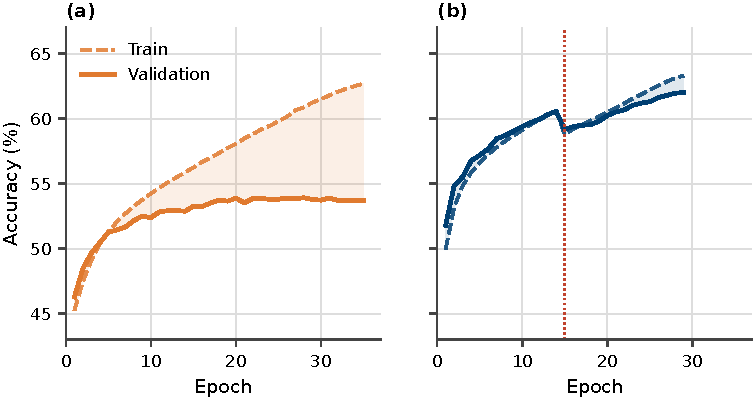
\includegraphics[width=\textwidth]{figures/training_dynamics.pdf}
    \caption{Training dynamics for v3 (500K, left), NT-Genus-5M (5M, centre), and NT-Genus (50M, right). Dashed lines show training accuracy; solid lines show validation accuracy. The shaded region highlights the train-validation gap. Dotted vertical lines mark learning-rate resets caused by SLURM timeout and job resumption; NT-Genus experienced two such resets (epochs 7 and 11) before the resume logic was corrected. Overfitting decreases systematically as data volume increases.}
    \label{fig:training-dynamics}
\end{figure}

\textbf{Conclusion}: All training techniques on the 500K dataset yield at most $\pm0.5$~pp improvement in RC TTA accuracy among the non-failed runs (range: 53.58\%--55.36\%). Inside this tokenizer and backbone, \emph{data volume}, not architecture or training tricks, is the bottleneck that the next section scales.

\section{Data Scaling Experiments}
\label{sec:exp-scaling}

Motivated by the accuracy plateau on 500K data and the comparison with MetaTransformer~\cite{Wichmann2023} (which trained on a large-scale balanced dataset trained on the full HGR-UMGS dataset of 2,505 species with coverage factor~4), we systematically scale training data.

\subsection{NT-Genus-5M: 5M Balanced Reads}

\subsubsection{Setup}

A 5M species-balanced subsample is drawn from the full 258M dataset. Each of 1,535 species contributes $\sim$3,257 reads, yielding near-perfect class balance. The v3 architecture and training configuration are retained (batch size 32, gradient accumulation 2, effective batch size 64), and training proceeds for 30 epochs.

Due to the 48-hour SLURM time limit, training required two jobs: the initial run completed 14 of 20 epochs before timeout, and a resumed run completed 16 additional epochs (epochs 15--30) using the \texttt{--resume} mechanism. A third job performed final evaluation.

\subsubsection{Results}

\begin{table}[htbp]
    \centering
    \caption{Genus classification results across data scales: v4 (500K), NT-Genus-5M (5M balanced), and NT-Genus (50M balanced).}
    \label{tab:v8-results}
    \small
    \setlength{\tabcolsep}{4pt}
    \begin{tabular}{lccccc}
        \toprule
        \textbf{Metric} & \textbf{v4 (500K)} & \textbf{NT-Genus-5M} & \textbf{$\Delta$\textsubscript{v4$\to$5M}} & \textbf{NT-Genus (50M)$^\dagger$} & \textbf{$\Delta$\textsubscript{5M$\to$50M}} \\
        \midrule
        Micro Accuracy (fwd)    & 53.75\% & 62.02\% & $+8.27$~pp & 66.29\%           & $+4.27$~pp \\
        Micro Accuracy (RC TTA) & 55.29\% & 63.05\% & $+7.76$~pp & \textbf{67.07\%}  & $+4.02$~pp \\
        Balanced Accuracy       & 25.23\% & 33.35\% & $+8.12$~pp & 39.91\%           & $+6.56$~pp \\
        F1 (weighted)           & 52.51\% & 61.06\% & $+8.55$~pp & 65.61\%           & $+4.55$~pp \\
        F1 (macro)              & 25.70\% & 37.97\% & $+12.27$~pp & \textbf{44.82\%} & $+6.85$~pp \\
        Top-3 Accuracy          & ---     & 81.70\% & ---        & 84.40\%           & $+2.70$~pp \\
        Top-5 Accuracy          & 82.91\% & 88.08\% & $+5.17$~pp & 90.03\%           & $+1.95$~pp \\
        Top-10 Accuracy         & 91.29\% & 94.23\% & $+2.94$~pp & 95.25\%           & $+1.02$~pp \\
        F1$=$0 classes          & 9       & 2       & $-7$       & \textbf{0}        & $-2$ \\
        Train-Val Gap           & 6.25\%  & 1.30\%  & $-4.95$~pp & $<$1\%            & --- \\
        \bottomrule
    \end{tabular}
    \begin{tablenotes}
        \small
        \item $\dagger$ NT-Genus final metrics (epoch~30, converged).
    \end{tablenotes}
\end{table}

The results reveal clear log-linear scaling behaviour:
\begin{enumerate}
    \item \textbf{Accuracy}: Each $10\times$ data increase yields a substantial but diminishing gain in RC TTA accuracy: $+7.76$~pp (500K$\to$5M) and $+4.02$~pp (5M$\to$50M). The sub-linear trend is consistent with logarithmic scaling laws.
    \item \textbf{Macro F1}: Data scaling disproportionately benefits rare classes: $+12.27$~pp at the first step and $+6.85$~pp at the second. At 50M reads, all 120 genera have non-zero F1 for the first time.
    \item \textbf{F1$=$0 classes}: The number of unclassifiable genera drops from 9 to 2 (NT-Genus-5M) and finally to 0 (NT-Genus), meaning every genus in the dataset is correctly predicted for at least some reads.
    \item \textbf{Overfitting}: The train-validation gap shrinks dramatically from 6.25\% (v4) to 1.30\% (NT-Genus-5M) to $<$1\% (NT-Genus), confirming that the model transitions from data starvation to well-generalised training as data volume increases.
\end{enumerate}

\subsubsection{Training Dynamics}

\begin{table}[htbp]
    \centering
    \caption{Training dynamics for NT-Genus-5M (5M balanced, 30 epochs). The gap between training and validation accuracy remains small throughout, in sharp contrast to the 500K experiments.}
    \label{tab:v8-dynamics}
    \begin{tabular}{ccccc}
        \toprule
        \textbf{Epoch} & \textbf{Train Acc} & \textbf{Val Acc} & \textbf{Train-Val Gap} & \textbf{Notes} \\
        \midrule
        1 & 49.96\% & 51.80\% & $-1.8$\% & \\
        5 & 55.97\% & 57.04\% & $-1.1$\% & \\
        10 & 58.93\% & 59.42\% & $-0.5$\% & \\
        14 & 60.60\% & 60.56\% & $+0.04$\% & 48h limit \\
        15 & 58.80\% & 59.18\% & $-0.4$\% & Resumed (LR reset) \\
        20 & 61.82\% & 60.59\% & $+1.2$\% & \\
        25 & 62.89\% & 61.77\% & $+1.1$\% & \\
        29$^\star$ & 63.32\% & 62.02\% & $+1.3$\% & Best epoch \\
        \bottomrule
    \end{tabular}
\end{table}

The temporary accuracy drop at epoch 15 is caused by the learning rate scheduler resetting to its warmup phase after resumption. The model recovers within 3--4 epochs and eventually surpasses the pre-interruption performance.

\subsection{NT-Genus Model: 50M Balanced Reads}
\label{sec:exp-v9}

Building on NT-Genus-5M, we scale training data by another $10\times$ to 50M balanced reads. The batch size is increased from 32 to 256 (with gradient accumulation reduced from 2 to 1, yielding an effective batch size of 256) to improve GPU utilization. The model is initialized from NT-Genus-5M's best checkpoint using \texttt{--init\_from} (transfer learning mode).

\begin{table}[htbp]
    \centering
    \caption{Configuration comparison between NT-Genus-5M and NT-Genus.}
    \label{tab:v9-config}
    \begin{tabular}{lcc}
        \toprule
        \textbf{Parameter} & \textbf{NT-Genus-5M} & \textbf{NT-Genus} \\
        \midrule
        Training reads & 4.5M & 45M \\
        Reads per species & $\sim$3,257 & $\sim$32,573 \\
        Batch size & 32 & 256 \\
        Gradient accumulation & 2 & 1 \\
        Effective batch size & 64 & 256 \\
        Epochs & 30 & 30 (converged) \\
        Weight initialization & Random & v8 best.pt \\
        Est.\ time per epoch & $\sim$3h & $\sim$5--6h \\
        \bottomrule
    \end{tabular}
\end{table}

\subsubsection{Results}

\begin{table}[htbp]
    \centering
    \caption{Comparison between NT-Genus-5M and NT-Genus (50M) for genus classification (120 classes).}
    \label{tab:v9-results}
    \begin{tabular}{lccr}
        \toprule
        \textbf{Metric} & \textbf{NT-Genus-5M} & \textbf{NT-Genus} & \textbf{$\Delta$} \\
        \midrule
        Micro Accuracy (fwd) & 62.02\% & \textbf{66.29\%} & $+4.27$~pp \\
        Micro Accuracy (RC TTA) & 63.05\% & \textbf{67.07\%} & $+4.02$~pp \\
        Balanced Accuracy & 33.35\% & 39.91\% & $+6.56$~pp \\
        F1 (weighted) & 61.06\% & 65.61\% & $+4.55$~pp \\
        F1 (macro) & 37.97\% & \textbf{44.82\%} & $+6.85$~pp \\
        Top-3 Accuracy & 81.70\% & 84.40\% & $+2.70$~pp \\
        Top-5 Accuracy & 88.08\% & 90.03\% & $+1.95$~pp \\
        Top-10 Accuracy & 94.23\% & 95.25\% & $+1.02$~pp \\
        F1$=$0 classes & 2 & \textbf{0} & $-2$ \\
        Best epoch & 29 & 30 (converged) & --- \\
        \bottomrule
    \end{tabular}
\end{table}

Scaling from 5M to 50M balanced reads yields a further $+4.02$~pp improvement in RC TTA accuracy (63.05\% $\to$ 67.07\%). Critically, the number of F1$=$0 classes drops to \textbf{zero}, indicating that all 120 genera are now correctly classified in at least some reads.

The marginal return diminishes relative to the previous $10\times$ scaling step: 500K$\to$5M yielded $+7.76$~pp while 5M$\to$50M yields $+4.02$~pp for the same multiplicative data increase, consistent with a logarithmic scaling relationship. This sub-linear trend is expected under log-linear scaling laws and suggests that continued data scaling alone will not close the remaining gap with MetaTransformer.

\paragraph{Training progress and LR restart incidents.}
NT-Genus training required multiple SLURM jobs due to the 48-hour time limit. Before a bug fix was applied to the checkpoint-resume logic, two job restarts inadvertently reset the cosine learning-rate scheduler to its initial warmup phase, causing temporary accuracy dips: $-0.54$~pp at epoch~7 and $-1.39$~pp at epoch~11. In both cases the model recovered within 3--5 epochs and surpassed the pre-dip performance level. The underlying issue---\texttt{EarlyStopping.best} being silently set to \texttt{None} from an incomplete checkpoint key---was corrected in the resume logic; from epoch~17 onward the scheduler state is correctly restored and the learning rate continues its cosine decay without interruption.

NT-Genus training completed at epoch~30 (April~2026), reaching a forward validation accuracy of \textbf{66.29\%} and RC~TTA accuracy of \textbf{67.07\%} (Figure~\ref{fig:learning-curves}). The learning curve plateaued between epochs~26 and~30 as the cosine schedule reached its minimum, indicating convergence.

\begin{figure}[htbp]
    \centering
    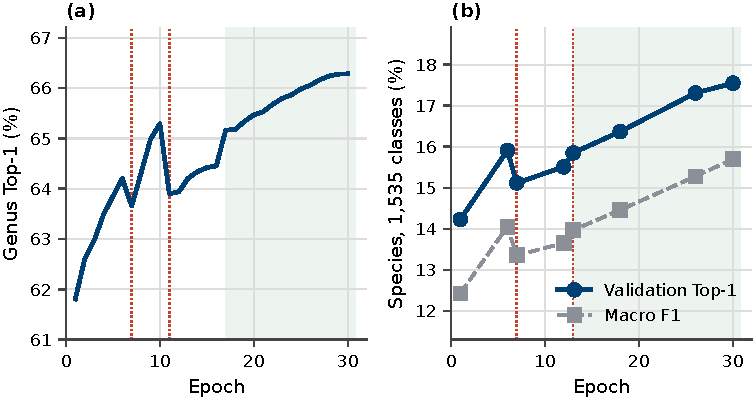
\includegraphics[width=0.95\textwidth]{figures/learning_curves.pdf}
    \caption{Full validation accuracy curves for NT-Genus (genus, left) and NT-Species (species, right) over all completed epochs. Red dotted vertical lines mark epochs where a SLURM job restart incorrectly reset the cosine LR scheduler, causing a temporary accuracy dip. The green shaded region indicates epochs trained after the resume bug fix was applied, during which the LR schedule correctly continues its cosine decay.}
    \label{fig:learning-curves}
\end{figure}

\subsection{Data Scaling Analysis}

\begin{table}[htbp]
    \centering
    \caption{Data scaling analysis: genus classification performance across data volumes. The 250M entry is the warm-started model (initialised from the 50M checkpoint and held out of the log-linear fit); the from-scratch 250M variant instead reaches 64.84\%. Only accuracy is reported for the 250M saturation experiment.}
    \label{tab:scaling}
    \begin{tabular}{rcccc}
        \toprule
        \textbf{Data Volume} & \textbf{RC TTA Acc} & \textbf{F1-macro} & \textbf{F1$=$0} & \textbf{Gap} \\
        \midrule
        500K (imbalanced) & 55.29\% & 25.70\% & 9 & 6.25\% \\
        5M (balanced) & 63.05\% & 37.97\% & 2 & 1.30\% \\
        50M (balanced) & \textbf{67.07\%} & \textbf{44.82\%} & \textbf{0} & $\sim$0.7\% \\
        250M (balanced, warm-start) & 67.29\% & --- & --- & --- \\
        MetaTransformer (HGR-UMGS full) & $\sim$98\% & --- & --- & --- \\
        \bottomrule
    \end{tabular}
\end{table}

The data scaling analysis reveals a clear relationship between training data volume and classification performance \emph{inside the NT-v2 6-mer framework}. The transition from 500K to 5M reads ($10\times$ increase) yields $+7.76$~pp in accuracy and $+12.27$~pp in macro F1. Meanwhile, all training technique ablations on the 500K dataset (v3--v7) produced at most $\pm0.5$~pp variation. Data volume, not architecture or training tricks, is therefore the primary determinant of 6-mer accuracy up to 50M. It is not the determinant of the residual gap to MetaTransformer: the 250M run below and Section~\ref{sec:exp-tokenization} show that gap is tokenizer-bound.

The published MetaTransformer genus recall of 98.3\% used a different data budget and tokenizer; it is not evidence that we simply need more 6-mer reads.

\figref{fig:data-scaling} plots genus RC TTA accuracy against training data volume on a logarithmic scale, with a log-linear fit to our three data points. The fitted curve projects that closing the gap with MetaTransformer would require training data well beyond our 50M-read scale, consistent with diminishing returns under logarithmic scaling.

\begin{figure}[htbp]
    \centering
    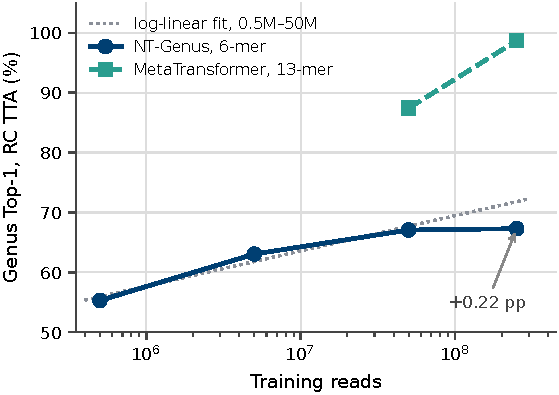
\includegraphics[width=0.80\textwidth]{figures/data_scaling.pdf}
    \caption{Genus RC TTA accuracy versus training data volume (log scale). The horizontal axis counts \emph{training reads including duplicates} (the per-epoch sample count); the corresponding \emph{unique}-read counts are smaller (50M$\to$17.8M, 250M$\to$41.9M unique, against a 42.6M source ceiling). Green circles mark our results at three data scales; the red star marks MetaTransformer's reported genus recall. The blue dashed line is a log-linear fit to our three data points. Per-$10\times$ accuracy gains diminish from $+7.76$~pp (500K$\to$5M) to $+4.02$~pp (5M$\to$50M). The fourth green circle (v15, 250M) continues the same warm-started series but is held out of the fit; at 67.29\% it falls well below the $\sim$71\% the log-linear fit would project at that scale---the trajectory flattens off its own projection, directly demonstrating that accuracy saturates beyond 50M rather than continuing along the trend. The MetaTransformer star marks reported genus recall (98.3\%); its x-position is based on training throughput (300K steps $\times$ batch~2,048) and is not directly comparable to our dataset-size axis.}
    \label{fig:data-scaling}
\end{figure}

\paragraph{Beyond 50M: the 6-mer model saturates, but the 13-mer model does not.}
The projection above tentatively attributes the residual gap to insufficient data. To test this directly, we scaled the balanced subsample by a further $5\times$ to 250M reads and trained two variants on a $64\times$H200 DDP cluster: a warm-started model initialised from the 50M NT-Genus checkpoint (mirroring the $5\text{M}\to 50\text{M}$ transfer) and a from-scratch model. Evaluated on an independent, read-disjoint test set under the identical RC-TTA protocol---on which the 50M NT-Genus model reproduces its $67.07\%$ to within $0.05$~pp---the 250M warm-started model attains only \textbf{67.29\%} genus Top-1 (RC~TTA), a $+0.22$~pp change over 50M despite the $5\times$ data increase, while the from-scratch 250M model is in fact lower at $64.84\%$. For the NT-v2 6-mer model, data scaling therefore \emph{saturates} beyond 50M rather than continuing along the log-linear trend.

Crucially, this saturation is a property of the \emph{tokenization}, not of the data or the single-genome-per-species reference. Trained on the \emph{same} reads, MetaTransformer with overlapping 13-mer tokenization continues to improve sharply with scale: on a common clean held-out pool its genus Top-1 rises from 87.5\% at 50M (the 87.42\% of Section~\ref{sec:exp-tokenization}) to \textbf{98.7\%} at 250M---and from 83.0\% to 98.5\% on a stricter ``leftover'' pool constructed to be sequence-ID-disjoint from both training sets, which rules out leakage. The identical $5\times$ data increase that moves the 6-mer model by $+0.22$~pp moves the 13-mer model by ${\sim}+11$~pp. The additional reads are therefore not redundant in any absolute sense: they carry discriminative signal that a non-overlapping 6-mer representation cannot resolve but an overlapping 13-mer one can. What saturates at 50M is the \emph{information ceiling of the 6-mer tokenizer}, not the data.

We therefore conclude that whether additional training data helps is governed by tokenization: the remaining gap to MetaTransformer is \emph{not} closable by additional data within the NT-v2 6-mer framework, whereas an overlapping long-$k$ tokenizer converts the same reads into near-perfect genus assignment. We caution, however, that the 98.7\% figure reflects \emph{near-complete closed-set coverage of the 1{,}535 reference genomes' 13-mer content}---at 250M reads the overlapping 13-mer model approaches a lookup over the known genomes---and does \emph{not} measure generalisation to novel, unseen genomes. The operative ceiling for our setting is thus tokenization (Section~\ref{sec:exp-tokenization}) rather than data volume.

\subsection{Balancing Axis: Species-Balanced vs.\ Genus-Balanced Training}
\label{sec:exp-genus-balance}

The scaling experiments above are species-balanced (each of the 1{,}535 species contributes equally). A natural alternative is to balance at the \emph{genus} level (each of the 120 genera contributes equally), which up-weights species-poor genera. To isolate the effect of the balancing axis alone, we trained two NT-v2 6-mer models on the \emph{same} 17.6M-read budget, differing only in this choice, and evaluated both on a common natural-abundance read pool. Table~\ref{tab:genus-balance} reports the result across three complementary metrics: per-read micro accuracy (the rate a randomly drawn read is classified correctly, the operationally relevant quantity for real samples), per-genus flat accuracy (macro-averaged over the 120 genera, treating each genus equally), and the Pearson correlation of estimated versus true relative abundance on real samples.

\begin{table}[htbp]
    \centering
    \caption{Effect of the training balancing axis at a fixed 17.6M-read budget (same reads, balancing differs only in whether species or genera are equalised). Genus-balancing trades a $+10$~pp gain in macro/flat accuracy for a $-23$~pp loss in per-read accuracy and a sharp drop in real-sample abundance fidelity.}
    \label{tab:genus-balance}
    \small
    \begin{tabular}{lccc}
        \toprule
        \textbf{Balancing} & \textbf{Per-read acc.} & \textbf{Per-genus flat acc.} & \textbf{Sample-level $r$} \\
        \midrule
        Species-balanced (sbal) & \textbf{60.4\%} & 33.1\% & \textbf{0.993} \\
        Genus-balanced (gbal)   & 37.2\% & \textbf{43.5\%} & 0.862 \\
        \bottomrule
    \end{tabular}
\end{table}

Two findings follow. First, genus-balancing is \emph{counterproductive for real metagenomics}: although it lifts the macro/flat accuracy that weights rare genera equally ($33.1\% \to 43.5\%$, $+10.4$~pp), it does so by sacrificing exactly the reads that dominate real samples---per-read accuracy collapses from $60.4\%$ to $37.2\%$ ($-23.2$~pp) and the relative-abundance correlation degrades from $r=0.993$ to $r=0.862$. Because real samples are dominated by abundant genera, the per-read and abundance metrics are the ones that matter operationally, and on both the species-balanced model is decisively better. Second, the per-genus flat accuracy plateaus at $\sim$42--43\% \emph{even when the training distribution is explicitly genus-balanced}. This ceiling is therefore not a fixable artefact of class imbalance; it reflects the intrinsic difficulty of resolving 120 genera from 150~bp reads under 6-mer tokenization---consistent with the train-fit ceiling of Section~\ref{sec:exp-tokenization}.

\section{RC Test-Time Augmentation Analysis}
\label{sec:exp-rc-tta}

\begin{table}[htbp]
    \centering
    \caption{Effect of RC TTA across experiments. RC TTA consistently improves accuracy at the cost of $2\times$ inference time.}
    \label{tab:rc-tta}
    \begin{tabular}{lccr}
        \toprule
        \textbf{Experiment} & \textbf{Fwd Only} & \textbf{RC TTA} & \textbf{$\Delta$} \\
        \midrule
        v3 (500K genus) & 53.92\% & 55.36\% & $+1.44$~pp \\
        v4 (500K genus) & 53.75\% & 55.29\% & $+1.54$~pp \\
        v5b (500K, LA $\tau$=0.3) & 52.29\% & 53.58\% & $+1.29$~pp \\
        v7 (500K, RC consist.) & 54.10\% & 55.18\% & $+1.08$~pp \\
        NT-Genus-5M (5M genus) & 62.02\% & 63.05\% & $+1.03$~pp \\
        NT-Genus (50M genus) & 66.29\% & 67.07\% & $+0.78$~pp \\
        NT-Genus (250M genus, warm-start) & 66.61\% & 67.29\% & $+0.68$~pp \\
        Shallow-Genus (50M genus, shallow) & 53.80\% & 53.88\% & $+0.08$~pp \\
        \bottomrule
    \end{tabular}
\end{table}

RC TTA provides a consistent $+1.0$ to $+1.5$~pp accuracy improvement across all experiments, regardless of the training configuration or data scale. Several observations merit discussion:

\begin{enumerate}
    \item \textbf{Biological basis}: As discussed in Section~\ref{sec:bg-rc-symmetry}, a metagenomic read and its reverse complement encode identical biological information. RC TTA exploits this strand symmetry by treating the two orientations as a two-view ensemble of the same underlying genomic entity~\cite{Zhou2022rc}.
    
    \item \textbf{Variance reduction}: The consistent improvement across all settings is explained by standard ensemble theory: averaging two correlated but independently noisy estimates of the same ground-truth label reduces prediction variance, even when both estimates come from the same model.
    
    \item \textbf{Diminishing returns with RC consistency training}: v7 (RC consistency, $+1.08$~pp) shows less benefit than vanilla models, because RC consistency training already encourages $f(s) \approx f(\bar{s})$ during training, leaving less residual strand asymmetry for RC TTA to correct.

    \item \textbf{Scale-dependent diminishing returns}: The RC TTA benefit decreases slightly with data scale: $+1.44$~pp at 500K, $+1.03$~pp at 5M, $+0.78$~pp at 50M, and $+0.68$~pp at 250M (NT-Genus). Larger training sets expose the model to both strands of each locus more often, gradually reducing systematic strand-directional errors---though a non-trivial asymmetry persists even at 50M reads.

    \item \textbf{Near-zero benefit for randomly initialized models}: Shallow-Genus (shallow Transformer, random initialization) shows only $+0.08$~pp from RC TTA. Without pre-training on a large genomic corpus, the model does not develop systematic strand-direction preferences, leaving little strand asymmetry for RC TTA to correct. This further supports the view that RC TTA primarily corrects pre-training-induced strand biases rather than stochastic inference noise.
\end{enumerate}

The $2\times$ inference cost is the primary trade-off. For offline evaluation this is acceptable; for latency-sensitive deployment, RC-equivariant architectures~\cite{Brown2021rc} or RC consistency regularization~\cite{Ma2025rc} may be preferred alternatives.

\figref{fig:rc-tta} summarises RC TTA gains across all experiments, highlighting the near-zero benefit for the randomly initialized Shallow-Genus model.

\begin{figure}[htbp]
    \centering
    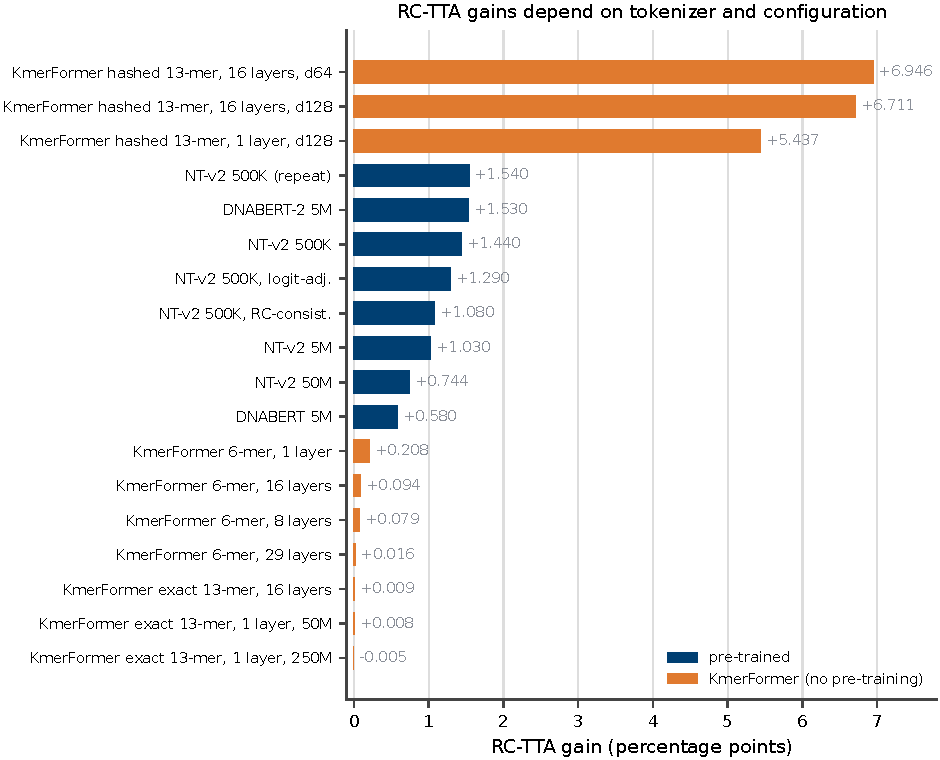
\includegraphics[width=\textwidth]{figures/rc_tta_benefit.pdf}
    \caption{RC TTA benefit across experiments. Top: forward-only vs.\ RC TTA accuracy (blue: NT-v2 backbone; green: DNABERT family; right of second dashed line: random init). Bottom: absolute gain in percentage points. NT-v2-based models gain $+0.77$--$+1.54$~pp consistently. DNABERT gains only $+0.58$~pp, likely because its overlapping 6-mer tokenization is inherently more RC-symmetric than NT-v2's non-overlapping 6-mer. DNABERT-2 (BPE tokenization) gains $+1.53$~pp, similar to early NT-v2 experiments. The randomly initialized Shallow-Genus gains only $+0.08$~pp, confirming that the benefit primarily corrects pre-training-induced strand biases.}
    \label{fig:rc-tta}
\end{figure}

\section{Computational Resource Analysis}
\label{sec:exp-resources}

\subsection{Observed Resource Usage}

\begin{table}[htbp]
    \centering
    \caption{Computational resource usage across experiments.}
    \label{tab:resources}
    \begin{tabular}{lrrr}
        \toprule
        \textbf{Metric} & \textbf{v3 (500K)} & \textbf{NT-Genus-5M} & \textbf{NT-Genus} \\
        \midrule
        GPU & V100 32GB & H100 80GB & H100 80GB \\
        Batch size & 32 & 32 & 256 \\
        VRAM peak (training) & 10.4 GB & $\sim$4.7 GB & $\sim$5 GB \\
        VRAM utilization & 32.5\% & 5.5\% & $<$7\% \\
        Train throughput & 1,128 r/s & $\sim$1,800 r/s & $\sim$1,825 r/s \\
        Inference throughput & --- & $\sim$5,100 r/s & $\sim$5,170 r/s \\
        Epoch time & $\sim$6.5 min & $\sim$6.8h & $\sim$6.9h \\
        Total training & 11.5h & $\sim$90h & $\sim$207h (30 ep.) \\
        SLURM jobs needed & 1 & 3 & 4+ \\
        \bottomrule
    \end{tabular}
\end{table}

\subsection{Bottleneck Analysis}

\begin{table}[htbp]
    \centering
    \caption{Resource bottleneck assessment on TWCC H100 nodes.}
    \label{tab:bottleneck}
    \begin{tabular}{lll}
        \toprule
        \textbf{Resource} & \textbf{Status} & \textbf{Assessment} \\
        \midrule
        GPU VRAM (80 GB) & $<$50\% utilized & No upgrade needed \\
        GPU compute (H100) & Adequate & No upgrade needed \\
        System RAM (128 GB) & $<$50\% utilized & No upgrade needed \\
        Storage & $<$10 GB per experiment & No upgrade needed \\
        \textbf{SLURM time (48h)} & \textbf{Primary bottleneck} & \textbf{Requires resume or longer limits} \\
        \bottomrule
    \end{tabular}
\end{table}

The hardware is substantially over-provisioned for this workload: the H100 80~GB GPU runs at $<$50\% VRAM utilization even with batch size 256, and system RAM usage is well within limits. The primary operational bottleneck is the 48-hour SLURM wall time limit, which necessitates multiple job submissions with checkpoint resumption for large-scale experiments.

\section{Comparison with MetaTransformer}
\label{sec:exp-comparison}

\begin{table}[htbp]
    \centering
    \caption{Comparison between our approach and MetaTransformer~\cite{Wichmann2023}.}
    \label{tab:metatransformer-comparison}
    \begin{tabular}{lcc}
        \toprule
        \textbf{Aspect} & \textbf{NT-Genus} & \textbf{MetaTransformer} \\
        \midrule
        Backbone & NT-v2 (498M) & Custom Transformer ($\sim$5M encoder$^\dagger$) \\
        Tokenization & 6-mer (pre-trained) & 12-mer (learned) \\
        Pre-training & Yes (850 genomes, MLM) & No (trained from scratch) \\
        Trainable params & 5.54M (LoRA) & $\sim$5M encoder$^\dagger$ (all) \\
        Training data & 50M balanced & HGR-UMGS full (2,505 sp., coverage 4) \\
        Genus accuracy & 67.07\% (RC TTA) & 98.3\% recall (val) \\
        Data source & HGR-UMGS + ART & HGR-UMGS + ART (same) \\
        \bottomrule
    \end{tabular}
    \begin{minipage}{\linewidth}
        \vspace{2pt}
        \footnotesize $^\dagger$Encoder parameters only; the embedding table is not counted here. For the overlapping 13-mer (stride~1) configuration, the embedding table alone is ${\sim}2.1$B parameters (see the parameter-accounting caveat below).
    \end{minipage}
\end{table}

Despite using a foundation model $100\times$ larger than MetaTransformer, our model (at 50M training reads) substantially underperforms MetaTransformer (trained on the full HGR-UMGS dataset). The key differences are:

\begin{enumerate}
    \item \textbf{Training data volume}: MetaTransformer uses the full HGR-UMGS dataset with coverage~4 vs. our 50M balanced reads. Inside the 6-mer framework each $10\times$ data increase yields $+3$--$8$~pp with diminishing returns, but the 250M run (Section~\ref{sec:exp-scaling}) shows that extra 6-mer data does not close this gap.
    
    \item \textbf{Training paradigm}: MetaTransformer trains all encoder parameters from scratch ($\sim$5M; the embedding table is additional---see parameter-accounting caveat below), while we fine-tune only 5.54M LoRA parameters of a 498M-parameter model.
    
    \item \textbf{Tokenization}: MetaTransformer uses 12-mer tokenization (capturing longer sequence patterns per token), while NT-v2 uses 6-mers.
\end{enumerate}

This comparison is confounded by three simultaneous differences: backbone depth (29 vs.\ 1 layer), pre-training (yes vs.\ no), and tokenization (6-mer vs.\ 12-mer overlapping). Sections~\ref{sec:exp-shallow} and~\ref{sec:exp-tokenization} separate these factors. Tokenization accounts for the larger share of the gap. The one-layer versus 29-layer comparison does \emph{not} isolate pre-training; the depth sweep in Section~\ref{sec:exp-shallow} does.

\paragraph{The ``$\sim$5M parameters'' figure counts only the encoder.}
The $\sim$5M parameter count attributed to MetaTransformer throughout this comparison refers to its \emph{transformer encoder} alone; it omits the token-embedding table, which for large-$k$ tokenization dominates the parameter budget. A learned $k$-mer embedding assigns a distinct vector to every $k$-mer observed in training, so the embedding matrix grows with the realized vocabulary. For the overlapping 13-mer (stride~1) configuration that attains 87.42\% at 50M and 98.7\% at 250M, the realized vocabulary reaches ${\sim}33.5$M distinct $k$-mers; at the embedding width $d_{\text{model}}{=}64$, the embedding matrix alone is ${\sim}33.5\text{M}\times 64 \approx 2.1$ billion parameters---roughly $4\times$ the size of the entire 498M-parameter NT-v2 backbone. The 13-mer model is therefore parameter-light only in \emph{compute} (a single shallow encoder block over short token sequences), while being parameter-\emph{heavy} in \emph{storage} (a multi-billion-entry lookup table). This is intrinsic to the approach: its discriminative power comes precisely from giving each long $k$-mer its own vector, which is also what inflates the table. A fair efficiency comparison must therefore weigh MetaTransformer's small compute footprint against this large embedding-memory cost, rather than citing the ${\sim}5$M encoder figure as the model's total size.

\section{Backbone Ablation: Depth, Then Pre-training}
\label{sec:exp-shallow}

A one-layer randomly initialized Transformer with the same 6-mer tokenizer and attention-pooling head as NT-v2 (Section~\ref{sec:method-shallow}) is the comparison originally used to ``isolate pre-training.'' It does not: encoder depth (29 vs.\ 1) and width ($d{=}1024$ vs.\ $d{=}128$) change at the same time as pre-training. We keep that comparison as a confounded baseline, then vary only depth.

\subsection{Confounded baseline: 29-layer NT-v2 vs.\ one-layer from scratch}

\begin{table}[htbp]
    \centering
    \caption{Confounded backbone comparison: NT-v2 (NT-Genus) vs.\ one-layer Transformer (Shallow-Genus). Tokenizer, head, and 50M reads are shared; depth, width, and pre-training are not.}
    \label{tab:shallow-design}
    \begin{tabular}{lcc}
        \toprule
        \textbf{Component} & \textbf{NT-Genus} & \textbf{Shallow-Genus} \\
        \midrule
        Tokenizer & 6-mer (NT-v2) & 6-mer (NT-v2) \\
        Encoder & 29-layer, $d{=}1024$ & 1-layer, $d{=}128$ \\
        Pre-training & MLM on 850 genomes & None \\
        Trainable params & 5.54M (LoRA) & $\sim$200K (all) \\
        Classification head & Attention pool (4 heads) & Attention pool (4 heads) \\
        Training data & 50M balanced & 50M balanced \\
        Batch size & 256 & 512 \\
        \bottomrule
    \end{tabular}
\end{table}

\begin{table}[htbp]
    \centering
    \caption{Confounded backbone results on the original 50M splits: pre-trained NT-v2 (NT-Genus) vs.\ one-layer Transformer (Shallow-Genus). The $-13.19$~pp RC-TTA gap is real; it is not an isolated pre-training effect.}
    \label{tab:v11-results}
    \begin{tabular}{lccr}
        \toprule
        \textbf{Metric} & \textbf{NT-Genus} & \textbf{Shallow-Genus} & \textbf{$\Delta$} \\
        \midrule
        Micro Accuracy (fwd) & 66.29\% & 53.80\% & $-12.49$~pp \\
        Micro Accuracy (RC TTA) & \textbf{67.07\%} & 53.88\% & $-13.19$~pp \\
        Balanced Accuracy & 39.91\% & 22.28\% & $-17.63$~pp \\
        F1 (macro) & 44.82\% & 25.78\% & $-19.04$~pp \\
        F1$=$0 classes & 0 & 3 & $+3$ \\
        RC TTA gain & $+0.78$~pp & $+0.08$~pp & --- \\
        Best epoch & 30 / 30 & 15 / 15 & --- \\
        Inference throughput & $\sim$5,170 r/s & $\sim$750,000 r/s & $\approx$145$\times$ \\
        VRAM (training) & $\sim$5 GB & $\sim$0.07 GB & --- \\
        \bottomrule
    \end{tabular}
\end{table}

NT-Genus outperforms Shallow-Genus by \textbf{13.19~pp} RC TTA (67.07\% vs.\ 53.88\%) on the original splits. Macro F1 drops more than micro accuracy ($-19.04$~pp vs.\ $-13.19$~pp). RC TTA is nearly ineffective for the randomly initialized model ($+0.08$~pp vs.\ $+0.78$~pp). Shallow-Genus is ${\sim}$145$\times$ faster at inference. None of these observations isolates pre-training from depth. Figure~\ref{fig:backbone-ablation} shows the same confounded pair.

\begin{figure}[htbp]
    \centering
    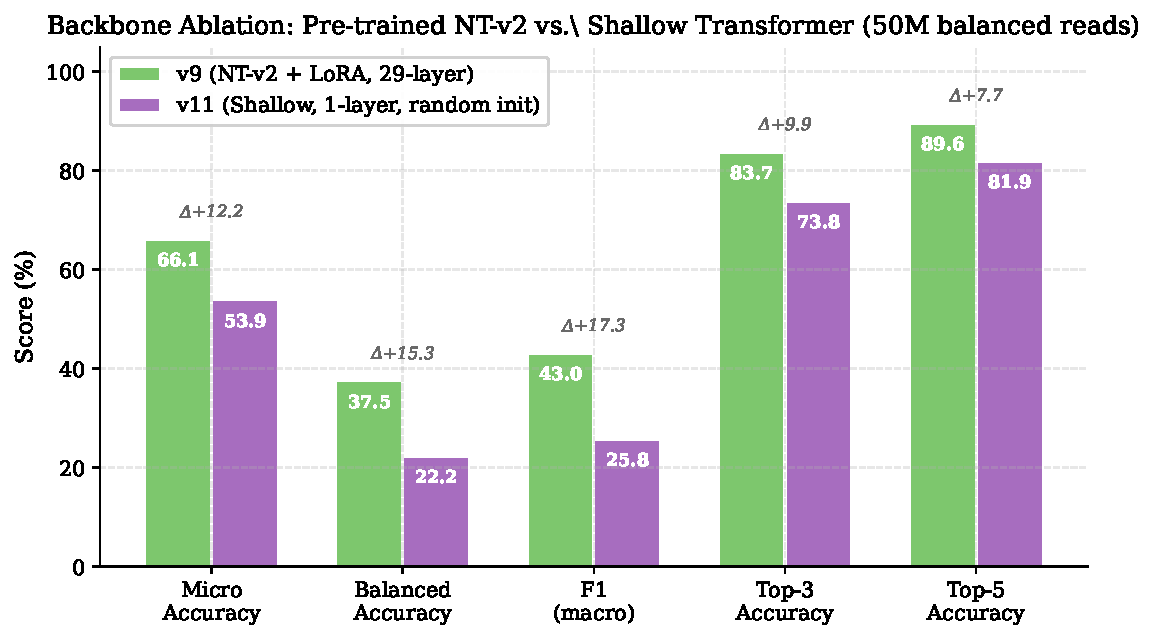
\includegraphics[width=0.90\textwidth]{figures/backbone_ablation.pdf}
    \caption{Confounded backbone comparison: pre-trained NT-v2 + LoRA (NT-Genus, green) vs.\ one-layer randomly initialized Transformer (Shallow-Genus, purple), both trained on 50M balanced reads. The gaps are real and include depth and width, not pre-training alone.}
    \label{fig:backbone-ablation}
\end{figure}

\subsection{Depth sweep at matched 6-mer tokenization}
\label{sec:exp-depth-sweep}

Table~\ref{tab:depth-sweep} holds the tokenizer (NT-v2 non-overlapping 6-mer), the 50M gut-read pool, the attention-pooling head, 15 training epochs, RC TTA, and the \texttt{clean\_common} 100K file fixed, and varies only encoder depth for the from-scratch models (Section~\ref{sec:method-shallow}). NT-v2 LoRA is the pre-trained reference on the same file.

\begin{table}[htbp]
    \centering
    \caption{Depth sweep, non-overlapping 6-mer, 50M gut reads, RC TTA on the same \texttt{clean\_common} 100K file. From-scratch models train 100\% of parameters. NT-v2 is LoRA-tuned (${\sim}$1\% of 500M).}
    \label{tab:depth-sweep}
    \small
    \begin{tabular}{lrrr}
        \toprule
        \textbf{Model} & \textbf{Params} & \textbf{Top-1} & \textbf{Balanced acc} \\
        \midrule
        1 layer, from scratch & 0.90M & 53.92\% & 0.220 \\
        8 layers, from scratch & 2.29M & 65.44\% & 0.388 \\
        16 layers, from scratch & 3.88M & \textbf{67.94\%} & \textbf{0.435} \\
        NT-v2, 29 layers, pre-trained + LoRA & 500M & 67.08\% & 0.398 \\
        \bottomrule
    \end{tabular}
\end{table}

Depth alone accounts for \textbf{+14.02~pp} (53.92\% $\to$ 67.94\%). That is larger than the $+13.19$~pp previously attributed to pre-training. The 16-layer from-scratch model \emph{exceeds} NT-v2 by $+0.86$~pp micro and $+3.7$~pp balanced accuracy with $129\times$ fewer parameters. A 3.88M-parameter model trained 100\% from scratch therefore matches the 6-mer ceiling of a 500M LoRA-tuned GFM; the ceiling is not an artefact of updating only ${\sim}$1\% of NT-v2. Neither from-scratch run had early-stopped at epoch 15, so the from-scratch numbers are lower bounds.

The one-layer re-run on \texttt{clean\_common} (53.92\%) agrees with the original Shallow-Genus 53.88\% on the internal split. NT-v2 on \texttt{clean\_common} (67.08\%) agrees with NT-Genus 67.07\%. The two pools match; the attribution does not.

For the 8-layer model, internal validation rose 0.634 $\to$ 0.654 from epoch 9 to 15 while \texttt{clean\_common} stayed at 65.44\%: the last six epochs memorised duplicated reads with no generalisation gain, consistent with the $6.07\times$ sequence-level redundancy in Section~\ref{sec:exp-setup}. Excluding the 0.17\% of \texttt{clean\_common} reads that share a \texttt{seq\_id} with training changes 65.44\% to 65.43\%.

\subsection{Data-efficiency crossover at matched depth}
\label{sec:exp-crossover}

The 50M result says pre-training does not raise the 6-mer ceiling. Table~\ref{tab:crossover-5m} asks whether it still helps when labels are scarce. A 16-layer from-scratch 6-mer model is trained on the same 5M gut reads used for NT-v2 v8 and scored on \texttt{clean\_common} with RC TTA.

\begin{table}[htbp]
    \centering
    \caption{Depth-matched 6-mer comparison at 5M gut reads (RC TTA). The 16-layer from-scratch model is scored on \texttt{clean\_common}. NT-v2 v8's 63.05\% is its recorded internal-validation figure (that checkpoint was not re-scored on \texttt{clean\_common}); models we could check agree across the two pools (8-layer 0.6539 / 65.44\%, 16-layer 0.6772 / 67.94\%, NT-v2 v9 0.6707 / 67.08\%), and the 16-layer 5M run itself scored 0.5411 on both.}
    \label{tab:crossover-5m}
    \small
    \begin{tabular}{lrr}
        \toprule
        \textbf{Model (5M, 6-mer)} & \textbf{Params} & \textbf{Top-1} \\
        \midrule
        8-layer from scratch & 2.29M & 53.62\% \\
        16-layer from scratch & 3.88M & 54.11\% \\
        NT-v2 v8, pre-trained + LoRA & 500M & \textbf{63.05\%} \\
        \bottomrule
    \end{tabular}
\end{table}

At 5M, going from 8 to 16 layers buys $+0.49$~pp; at 50M the same step is $+2.50$~pp. Depth needs data to pay off, so extra from-scratch depth would not close the low-data gap. Combined with Table~\ref{tab:depth-sweep}:

\begin{table}[htbp]
    \centering
    \caption{Depth-matched pre-training contribution (16-layer from-scratch vs.\ NT-v2, non-overlapping 6-mer). Pre-training buys data efficiency, not a higher 50M ceiling.}
    \label{tab:crossover-summary}
    \small
    \begin{tabular}{lccc}
        \toprule
        \textbf{Training reads} & \textbf{16-layer scratch} & \textbf{NT-v2} & \textbf{Net pre-training} \\
        \midrule
        5M  & 54.11\% & 63.05\% & \textbf{$+8.94$~pp} \\
        50M & \textbf{67.94\%} & 67.08\% & $-0.86$~pp \\
        \bottomrule
    \end{tabular}
\end{table}

Soil 50M comparisons of NT-v2 against a one-encoder-block MetaTransformer remain depth-confounded in the same way as Table~\ref{tab:v11-results}; they are not reported here as evidence for pre-training. Depth-matched soil controls were not completed.

\section{Tokenization Ablation: MetaTransformer at 50M Scale}
\label{sec:exp-tokenization}

The depth sweep (Section~\ref{sec:exp-shallow}) shows that, at matched 6-mer tokenization, pre-training does not raise the 50M ceiling. Tokenization is the remaining design difference relative to MetaTransformer. We first train the MetaTransformer architecture~\cite{Wichmann2023} on the same 50M balanced dataset under six tokenization configurations ($k \in \{6, 12, 13\}$, stride $\in \{1, k\}$), using the original MetaTransformer codebase on the Taiwania-2 cluster (V100 32~GB GPU). All configurations are evaluated on the same stratified 90/10 val split (5M reads). The 13-mer model uses \textit{embed\_dim}~$=$~64 to fit within V100 memory, consistent with the original MetaTransformer paper's 13-mer configuration~\cite{Wichmann2023}. A same-architecture 16-layer comparison in our codebase follows (Section~\ref{sec:exp-samearch-tok}).

\begin{table}[htbp]
    \centering
    \caption{Tokenization ablation (genus-level, 120 classes): NT-v2 + LoRA vs.\ MetaTransformer under six tokenization configurations. All MetaTransformer models are trained from scratch on 50M balanced reads. RC TTA is unavailable for MetaTransformer.}
    \label{tab:tokenization-ablation}
    \begin{tabular}{llccc}
        \toprule
        \textbf{Model} & \textbf{Tokenization} & \textbf{Tokens/read} & \textbf{Top-1 Acc} & \textbf{Macro F1} \\
        \midrule
        MetaTransformer & 13-mer, stride=1  & 138 & \textbf{87.42\%} & \textbf{0.7936} \\
        MetaTransformer & 12-mer, stride=1  & 139 & 78.83\% & 0.6531 \\
        NT-Genus & 6-mer, stride=6 & 25  & 67.07\%$^\dagger$ & --- \\
        NT-Genus & 6-mer, stride=6 & 25  & 66.29\% & 0.4384 \\
        MetaTransformer & 6-mer, stride=1   & 145 & 48.87\% & 0.1981 \\
        MetaTransformer & 6-mer, stride=6   & 25  & 47.00\% & 0.1682 \\
        MetaTransformer & 12-mer, stride=12 & 12  & 40.66\% & 0.0663 \\
        MetaTransformer & 13-mer, stride=13 & 11  & 27.30\% & 0.0182 \\
        \bottomrule
    \end{tabular}
    \begin{tablenotes}
        \small
        \item $\dagger$ RC TTA result (+0.78~pp over forward-only 66.29\%); MetaTransformer results are forward-only.
    \end{tablenotes}
\end{table}

\begin{table}[htbp]
    \centering
    \caption{Tokenization ablation (species-level, 1,535 classes): MetaTransformer under six tokenization configurations, trained on the same 50M balanced reads.}
    \label{tab:tokenization-ablation-species}
    \begin{tabular}{llccc}
        \toprule
        \textbf{Model} & \textbf{Tokenization} & \textbf{Tokens/read} & \textbf{Top-1 Acc} & \textbf{Macro F1} \\
        \midrule
        MetaTransformer & 13-mer, stride=1  & 138 & \textbf{49.62\%} & \textbf{0.4950} \\
        MetaTransformer & 12-mer, stride=1  & 139 & 16.79\% & 0.1439 \\
        MetaTransformer & 6-mer, stride=1   & 145 &  9.13\% & 0.0719 \\
        MetaTransformer & 6-mer, stride=6   & 25  &  6.44\% & 0.0470 \\
        MetaTransformer & 12-mer, stride=12 & 12  &  0.64\% & 0.0023 \\
        MetaTransformer & 13-mer, stride=13 & 11  &  0.51\% & 0.0026 \\
        \bottomrule
    \end{tabular}
\end{table}

Three independent effects can be read from Tables~\ref{tab:tokenization-ablation}--\ref{tab:tokenization-ablation-species}:

\paragraph{Effect of switching to the NT-v2 backbone (6-mer tokenization held; depth and codebase are not).}
NT-Genus (66.29\% forward) outperforms MetaTransformer with the same non-overlapping 6-mer tokenization (47.00\%) by \textbf{+19.29~pp}. This is an operational gap, not an isolated pre-training effect: MetaTransformer uses one encoder block, NT-v2 uses 29 layers, and the two codebases differ. Section~\ref{sec:exp-shallow} already showed that a 16-layer from-scratch 6-mer in our codebase reaches 67.94\%---above NT-v2---so MetaTransformer's 47.00\% 6-mer result understates the 6-mer ceiling. The number that isolates tokenization \emph{inside} MetaTransformer is the next paragraph, not this $+19.29$~pp.

\paragraph{Effect of tokenization (MetaTransformer architecture held constant).}
Tokenization design has a far larger effect than pre-training. Two sub-effects compound:
\begin{enumerate}
    \item \textbf{Stride (overlapping vs.\ non-overlapping)}: Across all $k$ values, overlapping stride$=$1 dominates non-overlapping stride$=k$. The gap widens dramatically with $k$: $+1.87$~pp for $k=6$, $+38.17$~pp for $k=12$, and $+60.12$~pp for $k=13$. Non-overlapping tokenization with large $k$ reduces each 150~bp read to as few as 11 tokens, discarding most sequence context.
    \item \textbf{k-mer length (overlapping only)}: Among stride$=$1 configurations, longer $k$ yields monotonically higher accuracy: 6-mer (48.87\%) $<$ 12-mer (78.83\%) $<$ 13-mer (87.42\%) at genus level, and 9.13\% $<$ 16.79\% $<$ 49.62\% at species level. Longer tokens are taxonomically more specific---hexamers are shared across distant taxa, while 12-mers and 13-mers increasingly identify individual lineages.
\end{enumerate}

\paragraph{Tokenization vs.\ NT-v2: MetaTransformer 13-mer.}
MetaTransformer with overlapping 13-mer tokenization, trained \emph{from scratch} on the 50M dataset (45M training reads), achieves \textbf{87.42\%} genus Top-1 accuracy---\textbf{+20.35~pp} above NT-Genus with RC TTA (67.07\%), with a transformer encoder ${\sim}100\times$ smaller and no pre-training (though its large-$k$ embedding table makes its \emph{total} parameter count far larger than NT-v2's; see the parameter-accounting caveat in Section~\ref{sec:exp-comparison}). Against the depth-matched 16-layer 6-mer (67.94\%), the best-vs-best gap is still ${\sim}$20~pp (87.42\% vs.\ 67.94\%), even though the 13-mer model uses one encoder block and the 6-mer model uses 16. At species level, MT 13-mer stride$=$1 reaches \textbf{49.62\%} (1,535 classes) on the 5M validation set and \textbf{49.74\%} on the independent 100K test set (Section~\ref{sec:spv4-hierarchical-prelim}), without any hierarchical routing. Task-specific tokenization is a more decisive factor than pre-trained prior knowledge for this task.

\paragraph{Decomposition from a common MetaTransformer 6-mer baseline.}
Because reverse-complement TTA is unavailable for MetaTransformer, Table~\ref{tab:pretraining-tokenization-decomp} changes one factor at a time from the from-scratch MetaTransformer non-overlapping 6-mer (47.00\% forward). The overlapping-12-mer and 13-mer rows hold the MetaTransformer architecture fixed and are therefore tokenization effects ($+31.83$~pp and $+40.42$~pp). The NT-v2 row does \emph{not} hold depth or codebase fixed; it is included only as the operational gap ($+19.29$~pp) that Section~\ref{sec:exp-shallow} already showed is not pre-training. Tokenization remains the largest single-factor change on this table.

\begin{table}[htbp]
    \centering
    \caption{Single-factor changes from a common from-scratch MetaTransformer 6-mer (non-overlapping) baseline at 50M reads (47.00\% forward genus Top-1). Overlapping 12-mer and 13-mer hold the MetaTransformer architecture fixed. The NT-v2 row additionally changes depth, width, pre-training, and codebase, and is not an isolated pre-training effect (Section~\ref{sec:exp-shallow}). All values are forward-only.}
    \label{tab:pretraining-tokenization-decomp}
    \small
    \begin{tabular}{lcc}
        \toprule
        \textbf{Single-factor change from MT 6-mer scratch (47.00\%)} & \textbf{Genus Top-1 (fwd)} & \textbf{$\Delta$} \\
        \midrule
        $+$ NT-v2 backbone (depth, pre-training, codebase also change)  & 66.29\% & $+19.29$~pp \\
        $+$ overlapping 12-mer tokenization (MT held)  & 78.83\% & $+31.83$~pp \\
        $+$ overlapping 13-mer tokenization (MT held)  & 87.42\% & $+40.42$~pp \\
        \bottomrule
    \end{tabular}
\end{table}

\paragraph{The bottleneck is representational: a train-fit ceiling.}
The decomposition above measures held-out accuracy, which conflates representational capacity with generalisation. A sharper test asks whether each model can fit its \emph{own training data}: a model that cannot separate the training set is limited by its input representation, not by capacity, data volume, optimisation, or overfitting. Table~\ref{tab:train-fit} reports training and validation accuracy at the largest (250M-read) scale. The NT-v2 6-mer models plateau at $63$--$66\%$ \emph{on the training set itself}, essentially equal to their validation accuracy (train--val gap ${\le}1$~pp)---they are not overfitting, they simply cannot fit. By contrast, MetaTransformer with overlapping 13-mer tokenisation fits the same task to $98.9\%$ training accuracy ($97.5\%$ validation).

The implication is decisive: with non-overlapping 6-mer tokenisation, reads from different genera are mapped to token sequences too similar to be separated, so no amount of additional capacity, data, or training can raise accuracy---the ceiling is imposed before learning begins, by the tokenizer. Overlapping 13-mers preserve enough sequence detail that the \emph{same model family} fits the data almost perfectly. This train-fit ceiling is the strongest single piece of evidence that tokenization, rather than backbone capacity or data volume, is the operative bottleneck for 6-mer GFMs on this task.

\begin{table}[htbp]
    \centering
    \caption{Train-fit ceiling at 250M reads: the 6-mer models cannot fit the training set beyond ${\sim}66\%$, whereas an overlapping 13-mer model fits it to ${\sim}99\%$. Training and validation accuracy are essentially equal for the 6-mer models, ruling out overfitting and isolating the input representation as the bottleneck. NT-v2 figures are forward micro-accuracy; the MetaTransformer training figure is micro-precision.}
    \label{tab:train-fit}
    \small
    \begin{tabular}{lccc}
        \toprule
        \textbf{Model (250M reads)} & \textbf{Train acc} & \textbf{Val acc} & \textbf{Train--val gap} \\
        \midrule
        NT-v2 6-mer, from scratch        & 63.2\% & 64.1\% & $-0.9$~pp \\
        NT-v2 6-mer, warm-start          & 65.8\% & 66.6\% & $-0.8$~pp \\
        MetaTransformer 13-mer (overlap) & \textbf{98.9\%} & \textbf{97.5\%} & $+1.4$~pp \\
        \bottomrule
    \end{tabular}
\end{table}

\paragraph{Convergence and capacity ceiling (12-mer).}
To determine whether 78.83\% is the true ceiling for the 12-mer model, training was extended into a second epoch. Train loss dropped sharply from 0.764 to 0.119, while validation loss \emph{worsened} from 1.203 to 2.288---immediate overfitting. The 50M-read dataset saturates the 5M-parameter single-encoder MetaTransformer within one epoch.

\paragraph{Overlapping tokenization within pre-trained GFMs (5M scale).}
The MetaTransformer ablation above is conducted entirely from scratch at 50M scale.
To isolate the effect of overlapping tokenization \emph{within the pre-trained GFM family}, we additionally fine-tune two other pre-trained DNA language models on the same 5M balanced dataset using identical training settings (LoRA $r=16$, attention-pooling head):
\begin{itemize}
    \item \textbf{DNABERT}~\cite{Ji2021}: BERT-base (86M params) pre-trained on the human reference genome with overlapping 6-mer tokenization (stride$=$1, 145 tokens per 150~bp read).
    \item \textbf{DNABERT-2}~\cite{Zhou2024dnabert2}: BERT-base (117M params) pre-trained on a multi-species genome collection using learned BPE tokenization ($\sim$34 tokens per read).
\end{itemize}

\begin{table}[htbp]
    \centering
    \caption{Pre-trained GFM backbone comparison at 5M balanced reads (genus-level, 120 classes).
    All models use LoRA $r=16$ fine-tuning and the same attention-pooling head.
    RC TTA is applied to all models.}
    \label{tab:backbone-tokenization-5M}
    \small
    \setlength{\tabcolsep}{4pt}
    \begin{tabular}{llcccc}
        \toprule
        \textbf{Model} & \textbf{Tokenization} & \textbf{Tokens/read} & \textbf{Params} & \textbf{RC TTA Acc} & \textbf{Macro F1} \\
        \midrule
        NT-Genus-5M  & 6-mer ($s{=}6$, non-overlap) & 25       & 499M & \textbf{63.05\%} & \textbf{0.449} \\
        DNABERT + LoRA     & 6-mer ($s{=}1$, overlap)     & 145      & 86M  & 61.78\%          & 0.384 \\
        DNABERT-2 + LoRA   & BPE                          & $\sim$34 & 117M & 58.88\%          & 0.323 \\
        \bottomrule
    \end{tabular}
\end{table}

Three observations follow from Table~\ref{tab:backbone-tokenization-5M}.

First, NT-Genus-5M with \emph{non-overlapping} 6-mer tokenization outperforms DNABERT with \emph{overlapping} 6-mer tokenization by $+1.27$~pp.
At 5M training reads, the pre-training advantage from NT-v2's larger backbone (499M vs.\ 86M parameters) and more diverse pre-training corpus (850 microbial genomes vs.\ human genome only) outweighs the tokenization benefit of overlapping stride.
This contrasts with the MetaTransformer results: when starting from scratch on the same data, overlapping tokenization provides a large benefit ($+1.87$~pp at $k=6$, $+60.12$~pp at $k=13$); but when starting from a strong pre-trained representation, the non-overlapping NT-v2 backbone already captures sufficient local context through its positional encodings.

Second, DNABERT with overlapping 6-mer tokenization (pre-trained, 86M, 5M data, 61.78\%) outperforms MetaTransformer with the same overlapping 6-mer tokenization (from scratch, one encoder block, 50M data, 48.87\%), despite ten times less training data.
This is an operational data-efficiency comparison at matched $k$; it is not depth-matched, and it should not be read as the isolated pre-training effect already measured in Section~\ref{sec:exp-crossover}.

Third, DNABERT-2's BPE tokenization (58.88\%) performs worse than either 6-mer model despite having a similar parameter count to DNABERT.
BPE segments DNA by frequency-based byte pairs rather than fixed-length k-mers, which may fragment taxonomically informative motifs; the learned vocabulary may not align well with the k-mer statistics that distinguish metagenomic reads.

\paragraph{Methodological note on training equivalence.}
The three models use the same learning rate ($5\times10^{-4}$ head/LoRA, $3\times10^{-5}$ backbone), warmup ratio (5\%), cosine decay schedule, and epoch count (30), but differ in batch size (NT-v2: 32, DNABERT: 128, DNABERT-2: 256) due to GPU memory constraints imposed by sequence length differences (25, 145, and $\sim$34 tokens per read respectively).
Consequently, the total number of gradient updates differs: approximately 453K for NT-v2, 117K for DNABERT, and 59K for DNABERT-2.
All three learning curves were still improving at epoch 30 (gain $<0.1$~pp per epoch), with the cosine schedule decaying the learning rate to near zero by the final epoch.
The comparison is therefore epoch-based---each model has seen the training data 30 times---rather than step-based or compute-matched.
This is standard practice in fine-tuning comparisons, and the observed ranking (NT-v2 $>$ DNABERT $>$ DNABERT-2) is unlikely to be reversed by additional training: DNABERT, despite receiving 3.9$\times$ fewer gradient updates than NT-v2, lags by only $1.27$~pp, while DNABERT-2's gap of $4.17$~pp is consistent across all training stages and attributable primarily to its BPE tokenization.

\paragraph{Sample-level evaluation of the three GFM backbones (5M scale).}
Read-level accuracy alone does not capture how a backbone choice propagates to the sample-level abundance and detection metrics that matter in practice.
We therefore apply the sample-level evaluation protocol (5M validation pool, 50K reads per sample, 100 partition samples; Section~\ref{sec:exp-sample}) to the RC-TTA predictions of all three pre-trained backbones at 5M scale.
Table~\ref{tab:backbone-sample-5M} reports the results.

\begin{table}[htbp]
    \centering
    \caption{Sample-level genus evaluation of the three pre-trained GFM backbones at 5M balanced reads (RC TTA predictions, 5M validation pool, 50K reads/sample).}
    \label{tab:backbone-sample-5M}
    \small
    \setlength{\tabcolsep}{5pt}
    \begin{tabular}{lccccc}
        \toprule
        \textbf{Model} & \textbf{Read Acc} & \textbf{Pearson $r$} & \textbf{Bray-Curtis} & \textbf{ROC AUC} & \textbf{Sens @ 95\% Spec} \\
        \midrule
        NT-Genus-5M       & \textbf{63.05\%} & \textbf{0.9928} & \textbf{0.112} & 0.666 & \textbf{14.5\%} \\
        DNABERT + LoRA    & 61.78\%          & 0.9906          & 0.113          & \textbf{0.672} & 14.2\% \\
        DNABERT-2 + LoRA  & 58.88\%          & 0.9915          & 0.141          & 0.640 & 11.6\% \\
        \bottomrule
    \end{tabular}
\end{table}

Two patterns emerge.
First, abundance estimation (Pearson $r$) saturates at $\sim$0.99 for all three backbones, consistent with the genus-level finding that relative-abundance correlation is forgiving at low task granularity (Section~\ref{sec:sample-mt-comparison})---the read-accuracy ranking (NT-Genus $>$ DNABERT $>$ DNABERT-2) does not separate the backbones on Pearson $r$.
Second, the discriminating metrics are Bray-Curtis dissimilarity and binary detection: DNABERT-2 is clearly worst on both (Bray-Curtis 0.141 vs.\ 0.112--0.113; ROC AUC 0.640 vs.\ 0.666--0.672; sensitivity at 95\% specificity 11.6\% vs.\ 14.2--14.5\%), mirroring its lower read accuracy and reinforcing that BPE tokenisation is the weakest of the three for this task.
NT-Genus and DNABERT are nearly indistinguishable at the sample level, with NT-Genus marginally ahead on Bray-Curtis and sensitivity and DNABERT marginally ahead on ROC AUC.

\paragraph{Same-architecture tokenizer comparison (16 layers).}
\label{sec:exp-samearch-tok}
The MetaTransformer $k$/stride grid holds one codebase fixed. Table~\ref{tab:samearch-tok} holds \emph{our} 16-layer encoder, the 50M gut-read pool, and \texttt{clean\_common} RC TTA fixed, and varies only the tokenizer (Section~\ref{sec:method-samearch-tok}). All three Taiwania-2 arms (Jobs~A/B/C) trained the full 15 epochs.

\begin{table}[htbp]
    \centering
    \caption{Same-architecture tokenizer comparison on 50M gut reads, scored on \texttt{clean\_common} 100K with RC TTA. The 16-layer non-overlapping 6-mer and 29-layer 6-mer rows are local runs; Jobs~A/B/C were trained on Taiwania-2. MetaTransformer 13-mer is the one-block published-protocol number from Table~\ref{tab:tokenization-ablation}, not a 16-layer run.}
    \label{tab:samearch-tok}
    \small
    \setlength{\tabcolsep}{3.5pt}
    \begin{tabular}{llrccc}
        \toprule
        \textbf{Model} & \textbf{Tokenizer} & \textbf{Params} & \textbf{Tok/read} & \textbf{Top-1} & \textbf{Bal.\ acc} \\
        \midrule
        16L from scratch & overlap 6-mer (Job~B) & 3.88M & 146 & 62.75\% & 0.353 \\
        16L from scratch & non-overlap 6-mer & 3.88M & 25 & 67.94\% & 0.435 \\
        29L from scratch & non-overlap 6-mer & 6.45M & 25 & 69.52\% & 0.462 \\
        NT-v2 + LoRA & non-overlap 6-mer & 500M & 25 & 67.08\% & 0.398 \\
        16L from scratch & hashed 13-mer, 2~GiB (Job~C) & 540M & 139 & 83.83\% & 0.669 \\
        16L from scratch & exact 13-mer, 8.6~GiB (Job~A) & 2.15B & 139 & 85.63\% & 0.732 \\
        MetaTransformer (1 block) & exact 13-mer & --- & 139 & 87.42\% & --- \\
        \bottomrule
    \end{tabular}
\end{table}

Four results follow.

(i)~\textbf{Long $k$ works at matched depth.} Hashed 13-mer reaches \textbf{83.83\%}---$+15.89$~pp over the 16-layer non-overlapping 6-mer and $+16.75$~pp over NT-v2---with a 2~GiB embedding rather than the 48~GiB a dense $4^{13}$ table would need. Hashing costs \textbf{1.80~pp} versus the exact table (85.63\%). Macro F1 rises faster than Top-1: overlapping 6-mer Job~B has macro F1 0.385, hashed 13-mer 0.732 ($1.90\times$), exact 13-mer 0.747. The 6-mer long tail, not just Top-1, is the tokenizer.

(ii)~\textbf{Depth compensates for a weak tokenizer.} With a 6-mer tokenizer, $1\to 29$ layers is worth $+15.60$~pp (53.92\% $\to$ 69.52\%). With a 13-mer tokenizer, MetaTransformer reaches 87.42\% with one encoder block while our 16-layer exact 13-mer reaches 85.63\%. Depth and pre-training were substituting for a representation that discards the signal. A one-layer hashed 13-mer in our codebase was not run; MetaTransformer's 87.42\% protocol is the 50M matched run in Table~\ref{tab:tokenization-ablation}, not an independent re-implementation.

(iii)~\textbf{Overlapping 6-mer is harmful.} Overlapping 6-mer (146 tokens) scores \textbf{62.75\%}, $-5.19$~pp against non-overlapping 6-mer (25 tokens) at far higher compute. $k$ length, not overlap at $k=6$, is what matters here. This does not contradict the MetaTransformer result that overlap is essential at $k=12$/$13$: those non-overlapping settings collapse to 11--12 tokens per read.

(iv)~\textbf{Caveats.} Job~A differs from B/C in exact vs.\ hashed vocabulary, $d_{\text{model}}$ 64 vs.\ 128 (memory-forced), and a canonical (RC-invariant) vocabulary. The width confound favours C, so the exact-vocabulary advantage is not a width artefact. Job~A ran fp16; B and C ran bf16. Only \texttt{evaluate.py --rc\_tta} on \texttt{clean\_common} 100K is comparable across arms. Canonical-vocabulary analysis predicted RC-TTA behaviour before the numbers existed: Job~A $+0.01$ (TTA is a no-op), Job~C $+6.71$ (non-canonical hashing), Job~B $-0.03$ (\texttt{rc\_augment} already taught invariance).

\paragraph{Implication for NT-v2.}
NT-v2 is constrained to 6-mer tokenization by its pre-training design. Switching to overlapping 13-mer tokenization on the same 50M reads yields $+15.89$~pp (hashed, 16-layer) to $+20.35$~pp (MetaTransformer) without using NT-v2 pre-training. A genomic foundation model pre-trained with overlapping long-$k$ tokenization on microbial genomes would combine that tokenizer with pre-training as a data-efficiency mechanism (Section~\ref{sec:exp-crossover}). General-purpose GFMs of the NT-v2/DNABERT family do not currently provide that combination; METAGENE-1 and GenomeOcean use BPE and were not tested (Chapter~\ref{ch:conclusion}).

\section{Species-Level Classification at Scale}
\label{sec:exp-species-scaled}

Genus accuracy saturates near 67\% under 6-mer tokenization (Section~\ref{sec:exp-scaling}). Species classification (1{,}535 classes) is the stricter test of whether the same representation can resolve intra-genus variation. A 500K pilot reached only 8.32\% direct Top-1 and 20.88\% under oracle-genus masking---far above chance (0.065\%) but too data-starved to interpret---so the remainder of this section uses the 50M scale.

\subsection{NT-Species at 50M}
\label{sec:spv4-final}

The species model is initialized from the NT-Genus backbone (\texttt{--init\_from}), transferring LoRA weights and replacing the 120-way head with a 1{,}535-way head. Training converged at epoch~30 (Figure~\ref{fig:learning-curves}, right panel) to \textbf{17.55\%} forward Top-1 on the 5M held-out set, with Top-3/5/10 of 31.26\%/38.19\%/47.65\%, balanced accuracy 17.56\%, macro F1 0.157, and 191/1{,}535 species at F1~$=$~0 (12.4\%). The same learning-rate restart that affected NT-Genus appeared at epoch~7 ($-0.79$~pp) and was corrected from epoch~13. Full-scale RC~TTA and routing on all 5M reads exceeded the 200~GB memory ceiling of the evaluation script (it materialises $5\text{M}\times 1{,}535$ logit arrays per mode); hierarchical comparisons therefore use the independent 100K set below. The genus-level RC~TTA gain is already measured at $+0.78$~pp (Section~\ref{sec:exp-v9}).

\subsection{Independent Test Set and Data-Leakage Audit}
\label{sec:spv4-data-leakage}

Hierarchical modes restrict the candidate set, so even modest train--test overlap can inflate oracle and per-genus scores. The 100K subset first used for these modes had been sampled from the training FASTA \emph{before} the train/validation split and shared $>$99\% of reads with the 45M training pool. We replaced it with 100K reads from MetaTransformer's \texttt{val\_reads.fa}---the same ART protocol and 2{,}505 HGR-UMGS genomes, 0\% overlap with our training stream. Re-scoring NT-Genus gave 66.6\% on the overlapping 100K versus 66.1\% on the independent 100K ($0.5$~pp); the NT-Species flat baseline moved by less than $0.4$~pp. That is evidence against read-level memorisation, but all hierarchical numbers below use the independent set. Genus results in Section~\ref{sec:exp-v9} use the standard 5M validation split and are unaffected.

\subsection{Hierarchical Evaluation}
\label{sec:spv4-hierarchical-prelim}

Table~\ref{tab:hierarchical-prelim} reports every routing mode on the independent 100K set. NT-Genus is 66.1\% on this set. The MetaTransformer hierarchical rows use one genus model plus per-genus logit masking, not a per-genus ensemble.

\begin{table}[htbp]
    \centering
    \caption{Species Top-1 on the independent 100K-read test set (1{,}535 classes). Per-genus (50M) is 81 dedicated NT-v2 heads with a frozen backbone. MT hierarchical uses a single genus router and species-logit masking.}
    \label{tab:hierarchical-prelim}
    \small
    \begin{tabular}{llcc}
        \toprule
        \textbf{Model} & \textbf{Mode} & \textbf{Top-1} & \textbf{F1 (macro)} \\
        \midrule
        NT-Species (ep30) & Flat & 15.9\% & 0.135 \\
        & Top-5 / soft genus routing & 15.9\% / 15.8\% & 0.136 / 0.135 \\
        & Oracle (true genus) & 27.4\% & 0.252 \\
        \midrule
        Per-genus (50M) & Predicted genus (NT-Genus) & 15.6\% & 0.152 \\
        & Oracle genus & 29.5\% & 0.283 \\
        \midrule
        MT 13-mer ($s{=}1$) & Flat / hierarchical (87.5\% genus) & 49.74\% / \textbf{50.86\%} & --- \\
        MT 6-mer ($s{=}1$) & Flat / hierarchical (48.9\% genus) & 9.22\% / 6.41\% & --- \\
        \bottomrule
    \end{tabular}
\end{table}

Four conclusions follow, and they are all that the extra routing experiments add.

\textbf{Per-genus specialisation is real under a perfect router.} Oracle-genus routing lifts the 81 per-genus 50M classifiers to 29.5\% Top-1 (macro F1 0.283), above the flat NT-Species oracle (27.4\%, F1 0.252). The specialists use a \emph{frozen} backbone, so the gain is from decomposing the 1{,}535-way problem, not from extra fine-tuning.

\textbf{Predicted routing does not realise that gain.} With NT-Genus (66.1\%), the per-genus pipeline is 15.6\%, $0.3$~pp \emph{below} the flat 15.9\% baseline. A wrong genus sends the read to a candidate set that cannot contain the true species. Flat top-5 / soft routing moves Top-1 by at most $0.1$~pp. The binding constraint is genus accuracy, not the species head.

\textbf{Tokenization sets a higher ceiling than routing can recover.} MT overlapping 13-mer, with no hierarchical routing, reaches \textbf{49.74\%} on the same set---$+20.2$~pp above the best NT-v2 number under any routing mode (29.5\%). The 6-mer intra-genus ceiling sits in the high-20s; long-$k$ tokenization more than doubles it.

\textbf{Masking helps only when the router is already strong.} MT 13-mer genus accuracy is 87.5\%, and masking adds $+1.12$~pp (49.74\%~$\to$~50.86\%). MT 6-mer genus accuracy is 48.9\%, and the same masking \emph{costs} $2.81$~pp (9.22\%~$\to$~6.41\%). NT-v2 sits in between: oracle $+11.5$~pp on the flat model, predicted routing $-0.3$~pp on the specialists. Hierarchical masking is beneficial if and only if it removes more wrong candidates than it accidentally excludes.

\label{sec:spv4-per-genus}
The 81 multi-species heads were trained on genus-scoped 50M subsets ($\sim$32{,}600 reads per species) with the backbone frozen; 39 singleton genera are assigned deterministically. Mean per-genus validation accuracy is 48.3\% (median 44.2\%), but four large genera dominate the error: \textit{Collinsella} (349 species, 1.3\%), \textit{Clostridium} (191, 19.9\%), \textit{Prevotella} (91, 26.6\%), and \textit{Bacteroides} (79, 15.9\%). Genera with $\leq$5 species average $>$80\%; those with $>$50 species average $<$20\%.

\subsection{Subgenus Routing: A Negative Result}
\label{sec:subgenus-routing}

We tested whether a $K$-means partition of NT-v2 embeddings ($\sim$25--30 species per subgroup, including \textit{Blautia}) could shrink those large genera. For \textit{Collinsella} the silhouette coefficient is $0.03$; a UMAP projection is an undifferentiated blob. Hard and soft subgenus routing both \emph{lower} species Top-1 relative to the per-genus baseline they were compared against (predicted 14.7\%~$\to$~13.2\%/13.6\%; oracle 27.8\%~$\to$~25.6\%/26.1\%). The finalised per-genus numbers in Table~\ref{tab:hierarchical-prelim} are 15.6\%/29.5\%; the negative conclusion is unchanged. Adding a routing tier without a representation that separates species is counterproductive. The bottleneck is 6-mer within-genus resolution, not hierarchy depth.

\section{Sample-Level Application Evaluation}
\label{sec:exp-sample}

Per-read accuracy is not the quantity most metagenomic studies report. This section asks whether the 67.07\% NT-Genus model, and the species models above, produce usable relative abundances and presence/absence calls. Metrics follow CAMI and Bracken practice~\cite{Sczyrba2017,Meyer2022cami2,Lu2017,McIntyre2017}: Pearson $r$ and Spearman $\rho$ for abundance, Bray--Curtis dissimilarity for magnitude-aware error, and ROC AUC for detection. All genus numbers reuse the NT-Genus RC~TTA predictions of Section~\ref{sec:exp-v9}; no extra GPU inference is required.

Two synthetic constructions are taken from the 5M validation pool (120 genera). \textbf{Random-partition} samples (100 $\times$ 50{,}000 reads) keep every genus present; because training is species-balanced, the expected abundance of genus $g$ is $n_g/1{,}535$. \textbf{Sparse-community} samples (200 $\times$ 50{,}000 reads) include exactly 60 of 120 genera, supplying true negatives for detection.

\subsection{Genus Abundance and Detection}
\label{sec:sample-abundance}
\label{sec:sample-detection}

On the 100 random-partition samples, NT-Genus yields Pearson $r = 0.9932$ (std $0.0004$), Spearman $\rho = 0.9312$ (std $0.0080$), and Bray--Curtis $0.0937$ (std $0.0017$). A 33\% per-read error rate still aggregates, because misclassifications spread across genera and largely cancel. High-abundance genera are slightly overestimated (classifier bias toward genera with more member species), not because of genome-length artefacts in the ART schedule (Section~\ref{sec:method-data}).

That $r = 0.993$ is \emph{not} a test of variable communities. Every partition sample shares the same expected abundance profile; the correlation measures stability under binomial sampling noise. Sparse-community detection is the stricter probe. With a $\geq$1-read call, sensitivity is 93.9\% at 0.01--0.1\% true abundance, 97.6\% at 0.1--1\%, and 100\% at $\geq$1\%. ROC AUC with predicted abundance as the score is $0.705$; sensitivity is 17.2\%/30.9\%/46.2\% at 95\%/90\%/80\% specificity. The modest AUC is a noise floor: at 33\% error, an absent genus in a 50{,}000-read sample is expected to receive $\sim 50{,}000 \times 0.33 / 120 \approx 138$ spurious reads ($\sim$0.28\%). A 95\%-specificity threshold must sit at 1.49\% predicted abundance and therefore also suppresses genuinely rare taxa. Abundance estimation is forgiving at 120 classes; calibrated presence/absence is not.

\subsection{Matched Protocol across Models}
\label{sec:sample-mt-comparison}

Table~\ref{tab:sample-model-comparison} repeats the same sample protocol for NT-Genus and two MetaTransformer checkpoints trained on the same 50M reads.

\begin{table}[htbp]
    \centering
    \caption{Genus sample-level evaluation under one protocol (100 partition samples, 200 sparse samples, 50K reads). Read accuracies are 67.07\% (NT-Genus, RC~TTA), 48.82\% (MT 6-mer $s{=}1$), and 87.42\% (MT 13-mer $s{=}1$).}
    \label{tab:sample-model-comparison}
    \begin{tabular}{lccc}
        \toprule
        \textbf{Metric} & \textbf{NT-Genus} & \textbf{MT 6-mer} & \textbf{MT 13-mer} \\
        \midrule
        Pearson $r$ (abundance)   & 0.993 & 0.984 & \textbf{0.999} \\
        Bray--Curtis              & 0.094 & 0.167 & \textbf{0.028} \\
        Sensitivity $\geq$1\%     & 100\% & 99.9\% & \textbf{100\%} \\
        Sensitivity 0.1--1\%      & 97.6\% & 86.8\% & \textbf{100\%} \\
        ROC AUC                   & 0.705 & 0.569 & \textbf{0.900} \\
        Sensitivity @ 95\% spec   & 17.2\% & 9.4\% & \textbf{47.7\%} \\
        \bottomrule
    \end{tabular}
\end{table}

Relative abundance at genus rank barely separates the methods ($r = 0.984$--$0.999$). Detection does: MT 13-mer AUC $0.900$ versus $0.705$/$0.569$ for the two 6-mer models, matching the noise-floor arithmetic (expected spurious reads fall from $\sim$138 at 67\% accuracy to $\sim$54 at 87\%). NT-Genus beats the from-scratch 6-mer MetaTransformer on every sample metric; the two models also differ in depth, width, and codebase, so this is an operational comparison at matched $k$, not an isolated pre-training effect (Section~\ref{sec:exp-shallow}).

\subsection{Species-Level Samples and Kraken2}
\label{sec:sample-species}

The independent 100K set has only $\sim$65 reads per species, so samples are smaller (1{,}000 reads; 100 partitions; 50 genera present in sparse samples). Table~\ref{tab:sample-species-comparison} keeps the rows that change the conclusion.

\begin{table}[htbp]
    \centering
    \small
    \caption{Species-level sample evaluation on the independent 100K set (1{,}535 classes, 1K reads/sample). Kraken\,2 uses a custom $k{=}35$ database from the same 2{,}505 UMGS+HGR genomes; unclassified reads (30\%) count in the denominator but add zero predicted abundance. The MT 13-mer hierarchical species checkpoint did not converge (val\_loss $= 9.29$ at batch 10{,}000) and is omitted here; its read-level numbers in Table~\ref{tab:hierarchical-prelim} remain valid.}
    \label{tab:sample-species-comparison}
    \begin{tabular}{lcccc}
        \toprule
        \textbf{Model} & \textbf{Read Acc} & \textbf{Pearson $r$} & \textbf{Bray--Curtis} & \textbf{ROC AUC} \\
        \midrule
        NT-Species flat & 17.8\% & 0.135 & 0.589 & 0.794 \\
        NT-Species hierarchical & 15.8\% & 0.106 & 0.608 & 0.796 \\
        Per-genus (predicted / oracle) & 15.6\% / 29.5\% & 0.083 / 0.159 & 0.625 / 0.541 & 0.789 / 0.842 \\
        MT 6-mer flat / hierarchical & 9.0\% / 6.4\% & 0.066 / 0.041 & 0.652 / 0.682 & 0.692 / 0.639 \\
        MT 13-mer flat & 53.7\% & \textbf{0.503} & \textbf{0.353} & 0.973 \\
        Kraken\,2 (in-DB) & \textbf{66.2\%} & \textbf{0.727} & \textbf{0.218} & 0.925 \\
        \bottomrule
    \end{tabular}
\end{table}

At 1{,}535 classes a 1{,}000-read sample gives $\sim$0.65 true reads per species. NT-Species at 17.8\% therefore has a noise floor ($\sim$0.54 spurious reads per species) comparable to the signal, and Pearson $r$ stalls at $0.135$. MT 13-mer at 53.7\% reaches $r = 0.503$. Species-level abundance becomes useful only around 40--50\% per-read accuracy---a threshold 6-mer models in this thesis never cross and overlapping 13-mer does. Predicted hierarchical masking again hurts when the router is weak (NT-Genus 66.1\%: $r$ $0.135\to 0.106$; MT 6-mer 48.9\%: $0.066\to 0.041$). Oracle per-genus routing is the NT-v2 ceiling ($29.5$\%, $r = 0.159$) and remains $24.2$~pp of read accuracy behind MT 13-mer flat.

Kraken\,2 on the same references reaches 66.2\% species Top-1 and $r = 0.727$, committing to 70\% of reads (94.6\% species / 99.3\% genus among those). The remaining 30\% abstain. Restricting to the 85{,}819 reads whose species are in the Kraken\,2 FASTA collection (219 of 1{,}535 species had no local assembly) raises Kraken\,2 to 77.18\% species Top-1 versus 52.64\% for MT 13-mer flat. At \emph{genus} rank the comparison flips for uncorrected Kraken\,2 counts (NT-Genus $r = 0.992$, MT 13-mer $r = 0.9993$, raw Kraken\,2 $r = 0.823$ on that restricted pool), but Bracken~\cite{Lu2017} restores Kraken\,2$+$Bracken to $r = 0.997$. Neural models therefore have \emph{no} sample-level abundance advantage against a standard Kraken\,2$+$Bracken pipeline on these simulated communities. What remains is (i)~read-level accuracy under a suitable tokenizer and (ii)~the fact that a neural classifier trains from labelled reads and does not need a per-species reference FASTA---Kraken\,2 accuracy on the 14{,}181 uncovered GCF reads is 0\% by construction, whereas those species are in-distribution for every neural model here.

The practical summary is short. Genus relative abundance on synthetic, near-balanced partitions cannot choose a method. Species abundance requires a tokenizer that already clears $\sim$50\% read accuracy. Hierarchical experts and subgenus routing do not lift a 6-mer GFM above that line. Kraken\,2$+$Bracken matches neural genus abundances on in-database simulated reads; learning-based methods earn their keep only where assemblies are missing or the tokenizer is long-$k$.

\section{Summary of Findings}

The experimental results lead to several key conclusions:

\begin{enumerate}
    \item \textbf{Inside a fixed 6-mer tokenizer, data volume dominates tricks}: A $10\times$ data increase yields $+7.76$~pp, while training-technique optimizations yield at most $\pm0.5$~pp. Beyond 50M the 6-mer model saturates ($+0.22$~pp at 250M); an overlapping 13-mer does not.

    \item \textbf{RC TTA is beneficial for pre-trained backbones}: Reverse-complement test-time augmentation consistently improves accuracy by $+0.1$--$1.5$~pp, with near-zero gain for randomly initialized models.

    \item \textbf{Class balance matters}: Balanced sampling across species eliminates the ``dead class'' problem (F1$=$0 classes: 9 $\to$ 2) and improves macro F1 ($+12.27$~pp).

    \item \textbf{Overfitting signals data starvation at 500K}: The train-validation gap shrinks from 6.25\% at 500K to 1.30\% at 5M.

    \item \textbf{The $+13.19$~pp one-layer gap is depth, not pre-training}: At matched 6-mer tokenization on \texttt{clean\_common}, 1 / 8 / 16 from-scratch layers score 53.92\% / 65.44\% / 67.94\% versus NT-v2 67.08\%. Depth accounts for $+14.02$~pp; pre-training at 50M is $\approx 0$. At 5M the same 16-layer match gives NT-v2 $+8.94$~pp (63.05\% vs.\ 54.11\%). Pre-training buys data efficiency, not a higher 6-mer ceiling.

    \item \textbf{Tokenization is the bottleneck, including at matched architecture}: Hashed 13-mer 16-layer reaches 83.83\% and exact 13-mer 85.63\%; MetaTransformer overlapping 13-mer reaches 87.42\%. A 29-layer from-scratch 6-mer reaches only 69.52\%. Overlapping 6-mer is harmful ($-5.19$~pp vs.\ non-overlapping).

    \item \textbf{Hardware is sufficient}: Current NVIDIA H100 hardware is adequately provisioned; the operational bottleneck is the SLURM time limit rather than computational resources.

    \item \textbf{Species hierarchy cannot outrun the tokenizer}: Per-genus specialists beat a flat oracle only when the genus is given (29.5\% vs.\ 27.4\%); predicted routing at 66.1\% genus accuracy does not (15.6\% vs.\ 15.9\%). Subgenus $K$-means on NT-v2 embeddings is a negative result. Overlapping 13-mer reaches 49.74\% flat---$+20.2$~pp above the best NT-v2 routing---and masking helps only when the genus router is already strong (Section~\ref{sec:spv4-hierarchical-prelim}).

    \item \textbf{Genus abundance cannot choose a method; species abundance can}: On synthetic partitions, Pearson $r$ is $0.984$--$0.999$ across 6-mer and 13-mer models. Species-level $r$ stays near $0.14$ until per-read accuracy crosses $\sim$40--50\%. Kraken2+Bracken matches neural genus abundances ($r = 0.997$); Kraken2 wins on in-database simulated species reads and is undefined on the 219 species without a local FASTA (Section~\ref{sec:exp-sample}).
\end{enumerate}
  % Experiments and Results
% !TeX root = ../main.tex

\chapter{Conclusion and Future Work}
\label{ch:conclusion}

\section{Summary of Contributions}

This thesis systematically evaluates the suitability of general-purpose genomic foundation models (GFMs) for metagenomic short-read taxonomic classification. Through controlled ablations of data scale, encoder depth, pre-training, and tokenization, we identify which design factors are decisive and which are not. Our main findings are:

\textbf{Tokenization sets the ceiling; data volume dominates only inside a fixed tokenizer.} Through systematic data scaling spanning 500K to 50M training reads, we show that within the NT-v2 6-mer framework, increasing training data by $10\times$ ($500\text{K}\to 5\text{M}$) yields $+7.76$~pp in accuracy and $+12.27$~pp in macro F1; a further $10\times$ ($5\text{M}\to 50\text{M}$) adds $+4.02$~pp. Pushing a further $5\times$ to 250M reads adds only $+0.22$~pp (67.29\%), empirically refuting the log-linear projection: the NT-v2 6-mer model saturates beyond 50M. This saturation is tokenizer-specific rather than a data limit: trained on the same reads over the same $50\text{M}\to250\text{M}$ range, an overlapping 13-mer model scales from 87.5\% to 98.7\% genus Top-1. By contrast, architectural and training-technique ablations on 500K reads yield at most $\pm0.5$~pp. The token-level pipeline---attention-pooling head fine-tuned with LoRA on the NT-v2 backbone---reaches 67.07\% genus Top-1 RC TTA at 50M reads, compared to 51.70\% for the frozen mean-pool baseline.

\textbf{The $+13.19$~pp one-layer gap is depth, not pre-training; pre-training buys data efficiency.} A 29-layer pre-trained NT-v2 versus a one-layer randomly initialized Transformer at the same 50M scale and 6-mer tokenizer differs by $+13.19$~pp RC TTA (67.07\% vs.\ 53.88\%). That comparison confounds pre-training with depth and width. A depth sweep with the tokenizer, data, head, and \texttt{clean\_common} evaluation held fixed scores 53.92\% / 65.44\% / 67.94\% at 1 / 8 / 16 from-scratch layers, against 67.08\% for NT-v2 LoRA: depth accounts for $+14.02$~pp ($1\to 16$), and at 50M the net contribution of pre-training is $\approx 0$ (the 3.88M-parameter 16-layer model is $+0.86$~pp higher). The 8- and 16-layer models are trained 100\% from scratch, so the $\sim$68\% 6-mer ceiling is not an artefact of LoRA updating only $\sim$1\% of NT-v2. The ranking reverses at 5M reads under the same 16-layer match: NT-v2 63.05\% versus from-scratch 54.11\% ($+8.94$~pp). Pre-training therefore helps when labels are scarce; it does not raise the 6-mer ceiling once 50M labelled reads are available. Within the family of pre-trained GFMs at 5M reads, NT-v2 still outperforms DNABERT by $+1.27$~pp and DNABERT-2 by $+4.17$~pp.

\textbf{Tokenization remains the dominant design factor, including at matched architecture.} Holding MetaTransformer fixed and varying $k \in \{6, 12, 13\}$ and stride, overlapping stride$=$1 is critical (up to $+60$~pp over non-overlapping at $k=13$), and longer $k$ yields monotonically higher accuracy among overlapping configurations. MetaTransformer with overlapping 13-mer tokenization, trained from scratch on the same 50M reads, achieves \textbf{87.42\%} genus Top-1---\textbf{+20.35~pp} above NT-v2 + LoRA (67.07\%). A same-architecture 16-layer comparison on \texttt{clean\_common} RC TTA reaches 83.83\% with a hashed 13-mer (2~GiB embedding) and 85.63\% with an exact 13-mer, versus 67.94\% for the 16-layer non-overlapping 6-mer; a 29-layer from-scratch 6-mer reaches only 69.52\%. Even when the 6-mer model is given 16 layers and the 13-mer MetaTransformer only one, the 13-mer still wins by $\sim$20~pp (87.42\% vs.\ 67.94\%). Depth compensates for a weak tokenizer; it does not break the 6-mer ceiling. MetaTransformer's published advantage on this task is therefore its 13-mer tokenizer, not a uniquely strong encoder.

\textbf{RC TTA is a robust, free improvement.} Reverse-complement test-time augmentation consistently improves accuracy by $+0.1$ to $+1.5$~pp across experimental conditions, requiring no additional training cost. The benefit is largest for pre-trained backbones ($+0.78$ to $+1.54$~pp) and near-zero for randomly initialized models ($+0.08$~pp), supporting the interpretation that RC TTA primarily corrects pre-training-induced strand biases rather than stochastic inference noise.

\textbf{Class balance is critical for rare taxa.} Balanced subsampling across species reduces the number of F1$=$0 classes from 9 to 2 and improves macro F1 by $+12.27$~pp, demonstrating that class imbalance---not model capacity---is the primary cause of poor performance on rare taxa at the 500K--5M scales.

\textbf{Per-genus specialisation validates the hierarchical architecture; subgenus routing does not.} Evaluation on a 100K independent test set demonstrates that per-genus 50M LoRA classifiers under oracle-genus routing reach 29.5\% species Top-1, exceeding the flat sp\_v4 oracle ceiling of 27.4\%. Predicted routing through the 66.1\%--67.07\% genus model lowers Top-1 to 15.6\%, marginally below the flat baseline (15.9\%), because per-genus specialists do not recognise reads from genera they were not trained on. Subgenus $K$-means routing on NT-v2 embeddings is a negative result (oracle Top-1 25.6--26.1\%).

\textbf{Per-read accuracy translates to sample-level utility under controlled conditions, but genus abundance cannot choose a method.} On synthetic species-balanced random-partition samples, 67\% per-read accuracy yields Pearson $r = 0.993$ for relative abundance and Bray-Curtis dissimilarity 0.094; 100\% detection sensitivity is achieved for taxa at $\geq$1\% relative abundance. All 100 random-partition samples share the same expected per-genus abundance profile, so this result measures stability under binomial sampling noise rather than generalisation to genuinely variable communities. Kraken2+Bracken matches neural genus abundances ($r = 0.997$) on these simulated communities. Evaluation on real and compositionally diverse microbiome samples remains an open question.

\section{Limitations}

This work has several limitations that should be acknowledged:

\begin{enumerate}
    \item \textbf{Simulated data only}: All experiments use reads simulated by ART from reference genomes. Real metagenomic reads contain additional noise (host contamination, chimeric reads, strain-level variation) that may degrade classifier performance.
    
    \item \textbf{Limited taxonomic scope}: The reference database covers 120 genera and 1,535 species of human gut microorganisms. Performance on environmental samples with broader taxonomic diversity is unknown.
    
    \item \textbf{Single read length}: All experiments use 150~bp reads. Performance at other read lengths (e.g., 250~bp for Illumina MiSeq, or long reads from Oxford Nanopore / PacBio) has not been evaluated.
    
    \item \textbf{Data scaling saturates for the 6-mer model, not universally}: We trained balanced subsets up to 250M reads (Section~\ref{sec:exp-scaling}); the warm-started 250M NT-v2 model reaches only 67.29\% RC TTA ($+0.22$~pp over the 50M 67.07\%), confirming that the 6-mer model saturates rather than following the log-linear projection. This is a limit of the tokenizer, not the data: trained on the same reads over the same range, an overlapping 13-mer model scales from 87.5\% to 98.7\% genus Top-1. The gap to overlapping-$k$-mer methods is therefore not closable by additional training data within the NT-v2 6-mer framework. We note that the 13-mer model's 98.7\% reflects near-complete closed-set coverage of the 1{,}535 reference genomes' 13-mer content (approaching a lookup over known genomes), and does not measure generalisation to novel genomes.

    \item \textbf{Memory-bound loader in the primary pipeline}: The single-GPU TWCC pipeline loads training reads into memory; the 250M-scale experiments above were instead run on a multi-GPU H200 cluster with a lazy, index-based loader. Unifying the two (a streaming loader in the main codebase) remains future engineering work.
    
    \item \textbf{Architectural capacity ceiling of MetaTransformer}: MetaTransformer's single-encoder-block design (${\sim}$5M encoder parameters, excluding the embedding table) saturates within one training epoch on 50M reads; a second epoch produces overfitting rather than further generalisation. A larger model would likely improve beyond 78.83\% at 12-mer but was not evaluated due to infrastructure constraints.

    \item \textbf{Scope is general-purpose GFMs}: We evaluated NT-v2 and, at 5M scale, DNABERT and DNABERT-2---models pre-trained for eukaryotic or mixed-genome regulatory genomics, not for short-read metagenomic taxonomy. Two GFMs pre-trained on metagenomic sequence were not tested: METAGENE-1~\cite{Liu2025metagene} ($\sim$1.5~Tbp wastewater metagenomes, BPE) and GenomeOcean~\cite{Zhou2025genomeocean} ($\sim$600~Gbp metagenomic assemblies, 4B parameters, BPE). The domain and context-length mismatch that plausibly explains NT-v2's $\approx 0$ transfer at 50M would not apply to those models in the same way, and their BPE tokenizers would introduce a further variable. Claims in this thesis are therefore scoped to general-purpose GFMs, not to all GFMs.

    \item \textbf{Remaining confounds in the tokenizer comparison}: The same-architecture 16-layer 13-mer arms differ in exact versus hashed vocabulary, embedding width ($d_{\text{model}}$ 64 vs.\ 128), and canonical versus non-canonical vocabulary; Job~A ran fp16 and Jobs~B/C ran bf16. MetaTransformer's 87.42\% is quoted from the matched 50M protocol used in Chapter~\ref{ch:experiments}; a one-layer hashed 13-mer in our own codebase was not run. Soil depth-matched from-scratch controls were not completed.

    \item \textbf{LoRA versus full fine-tune}: NT-v2 is adapted with LoRA on $\sim$1\% of parameters. A full fine-tune might score higher. The from-scratch 8- and 16-layer models, which train 100\% of parameters and hit the same $\sim$68\% 6-mer ceiling, are the evidence that the ceiling is not solely a LoRA artefact.
\end{enumerate}

\section{Future Work}

The findings above point to four primary future directions:

\subsection{Microbial Foundation Models with Overlapping Long-$k$ Tokenization}

The tokenization ablation (Section~\ref{sec:exp-tokenization}) identifies overlapping long-$k$ tokenization as the dominant performance driver. No publicly available GFM that we evaluated combines this property with large-scale pre-training on diverse microbial genomes; METAGENE-1 and GenomeOcean use BPE rather than long $k$-mers and were not tested here. The most promising direction consistent with the measurements in this thesis is therefore to pre-train a transformer on the GTDB database~\cite{Parks2022} ($>$400,000 microbial genomes) with overlapping 12-mer or 13-mer tokenization---or to evaluate hashed long-$k$ embeddings, which reached 83.83\% at 16 layers with a 2~GiB table. Open empirical questions include (i)~whether RC TTA provides an equivalent benefit ($\sim+1$~pp) at $k = 12$/13, (ii)~whether $k > 13$ continues to improve accuracy, (iii)~whether a one-layer hashed 13-mer in our codebase matches MetaTransformer's 87.42\%, and (iv)~whether BPE models pre-trained on metagenomes (METAGENE-1, GenomeOcean) close the 50M gap that NT-v2 does not. A complementary, lower-cost direction is to fine-tune NT-v2 with a learned 12-mer projection layer; this is bounded above by the model's pre-trained 6-mer positional encodings and is therefore expected to be a partial mitigation rather than a full solution.

\subsection{Streaming Infrastructure for Species-Level Scaling}

The genus-level data-scaling question is now settled: scaling balanced reads from 50M to 250M yields only $+0.22$~pp (Section~\ref{sec:exp-scaling}), so additional \emph{genus} training data is not a productive direction within the 6-mer framework---the earlier log-linear projection into the 82--90\% range is empirically refuted (an overlapping 13-mer tokenizer, by contrast, keeps improving on the same data; Section~\ref{sec:exp-scaling}). The streaming/DDP infrastructure built for the 250M runs nonetheless remains valuable for the \emph{species}-level task (1{,}535 classes), where per-species 50M and full-scale species training are still bottlenecked by the memory-bound primary pipeline. Folding the lazy, index-based loader and multi-GPU orchestration used here into the main codebase would enable those species-level experiments without re-introducing the in-memory ceiling.

\subsection{Hierarchical Routing Improvements for Species Classification}

Per-genus 50M classifiers under oracle-genus routing reach 29.5\% species Top-1 (Section~\ref{sec:spv4-hierarchical-prelim}), exceeding the flat sp\_v4 oracle (27.4\%) and validating per-genus specialisation. Predicted routing through the 66\%--67\% genus model, however, lowers Top-1 to 15.6\%---marginally below the flat baseline (15.9\%)---because per-genus specialists do not recognise reads from genera they were not trained on.

A subgenus routing tier was investigated as a direct approach to reducing intra-classifier confusion for the five largest genera (Section~\ref{sec:subgenus-routing}). Species-level $K$-means partitioning on NT-v2 embeddings was used to define subgroups of $\sim$25--30 species. Silhouette analysis (Collinsella: 0.03) and UMAP visualisation confirm that NT-v2's 6-mer representations do not separate species within a genus, and both hard and soft subgenus routing decreased oracle Top-1 to 25.6--26.1\% (below the per-genus baseline), indicating that adding a routing tier without better representations is counterproductive.

The primary path to improving hierarchical species accuracy is therefore to improve the quality of the genus router itself. Since NT-v2's 6-mer tokenisation constrains genus accuracy to $\sim$67\%, this is best addressed through the long-$k$ pre-training direction above: a microbial foundation model with overlapping 13-mer tokenisation would simultaneously increase genus routing accuracy and provide richer intra-genus representations that could support a meaningful subgenus partition.

\subsection{Real-World Validation and Calibrated Sample-Level Estimation}

Validation on real metagenomic data from public repositories (e.g., the Human Microbiome Project~\cite{HMP2012}) is essential for assessing practical applicability. This includes (i)~robustness to sequencing errors and platform-specific quality profiles, (ii)~handling host DNA contamination, and (iii)~out-of-distribution detection for taxa absent from the training database. In parallel, the random-partition abundance evaluation in Section~\ref{sec:exp-sample} measures stability under fixed expected composition rather than generalisation across compositionally variable communities; future evaluation should therefore use sparse, asymmetric, and real microbiome-derived sample compositions, paired with (iv)~calibrated statistical tests for presence/absence above the per-sample noise floor and (v)~learned abundance correction that compensates for the observed systematic overestimation of high-abundance genera (Section~\ref{sec:sample-abundance}).

\section{Concluding Remarks}

This thesis demonstrates both the promise and the current limitations of applying general-purpose genomic foundation models to metagenomic taxonomic classification. The controlled ablation experiments yield two concrete findings that extend beyond the specific system studied here.

First, tokenization---not pre-training, depth, or further 6-mer data---sets the closed-set genus ceiling on 150~bp reads. Four architecturally different non-overlapping 6-mer models cap at 65--70\% (8-layer from scratch 65.44\%, 16-layer 67.94\%, NT-v2 LoRA 67.08\%, 29-layer from scratch 69.52\%), while overlapping 13-mer models on the same 50M reads reach 83.83\% (hashed, 16-layer), 85.63\% (exact, 16-layer), and 87.42\% (MetaTransformer, one encoder block). The previously quoted $+13.19$~pp and $+19.29$~pp ``pre-training'' gaps compared a deep pre-trained model with a one-layer from-scratch model and do not survive a depth-matched control.

Second, pre-training is not useless: at matched 16-layer depth and 6-mer tokenization it is worth $+8.94$~pp at 5M reads, and near zero (slightly negative) at 50M. That is a data-efficiency result, not a ceiling result. Combined with NT-v2's pre-training context of 2{,}048 tokens ($\sim$12{,}288~bp) versus the 25 tokens (150~bp) used here, and with a pre-training corpus and benchmark suite aimed at regulatory genomics rather than short-read taxonomy, the prescription is specific: keep pre-training as a mechanism, but pre-train on short microbial reads with overlapping long $k$-mers (or a hashed equivalent), rather than expecting a larger eukaryote-regulatory GFM to close the gap.

Realising that direction, evaluating metagenome-pre-trained BPE models that were out of scope here, and completing species-level scaling and real-community sample evaluation, represent the most promising path toward a competitive, generalisable GFM-based metagenomic classifier.
  % Conclusion and Future Work

% References
\refmatter
\printbibliography

% Appendices
\appendix
\begin{appendices}
% !TeX root = ../main.tex

\chapter{Code and Data Availability}
\label{app:availability}

\section{Code Availability}
\label{sec:code-availability}

All source code, model definitions, training and evaluation scripts, and the complete set of experiment configuration files are publicly available at:

\begin{center}
\url{https://github.com/m2lab-ntu/gfm-classifier}
\end{center}

The repository contains, in addition to the training and inference pipeline, the full YAML configuration for every experiment reported in Chapter~\ref{ch:experiments} (the \texttt{v8}--\texttt{v15} runs spanning the 5M--250M read scales, the from-scratch and warm-start NT-v2 variants, and the MetaTransformer 13-mer baseline), under \texttt{configs/}. Each configuration records the backbone, the attention-pooling head dimensions, the LoRA settings ($r{=}16$, $\alpha{=}32$, applied to the query/key/value projections), the optimisation schedule, and the reverse-complement test-time augmentation flag, so that any reported result can be reproduced from the corresponding config and checkpoint. The headline hyperparameters are summarised in Tables~\ref{tab:lora-config} and~\ref{tab:training-config} of Chapter~\ref{ch:methodology}.

The repository also provides the distributed-training launch scripts used for the large-scale (250M-read) runs, which employ multi-GPU \texttt{DistributedDataParallel} rather than the single-device setting used for the smaller experiments.

\section{Data Availability}
\label{sec:data-availability}

The reference genome set (1{,}535 microbial genomes) is drawn from publicly available assemblies; the accession list, the read-simulation procedure, and the scripts used to construct the balanced and natural-abundance read sets (including the unique-read accounting for the 50M and 250M training pools) are included in the repository above under \texttt{data/}. Processed read sets and trained checkpoints are available from the author on reasonable request.

% % !TeX root = ../main.tex

\chapter{Supplementary Tables}
\label{app:tables}

This appendix collects tables that document the experiments in full but are not
needed to follow the argument of Chapter~\ref{ch:experiments}: the training
configurations of the early runs, the complete metric profile of the
species-level model, and the two large sample-level comparison tables whose
headline rows are quoted in Section~\ref{sec:exp-sample}.

\section{Training Configurations}
\label{app:configs}

\begin{table}[htbp]
    \centering
    \caption{Hyperparameter configurations for initial architecture experiments (500K dataset). Bold values indicate the setting that changed relative to v1.}
    \label{tab:v1-v3-configs}
    \begin{tabular}{lccc}
        \toprule
        \textbf{Hyperparameter} & \textbf{v1} & \textbf{v2} & \textbf{v3 (best)} \\
        \midrule
        Backbone LR & $5 \times 10^{-5}$ & $2 \times 10^{-5}$ & $3 \times 10^{-5}$ \\
        Head LR & $5 \times 10^{-4}$ & $3 \times 10^{-4}$ & $5 \times 10^{-4}$ \\
        RC augmentation & No & \textbf{Yes} & \textbf{Yes} \\
        Class weights & No & \textbf{Yes (capped@10)} & No \\
        Label smoothing & 0.0 & \textbf{0.1} & 0.0 \\
        Weight decay & 0.01 & 0.05 & 0.02 \\
        Head dropout & 0.1 & 0.2 & 0.15 \\
        LoRA dropout & 0.05 & 0.1 & 0.05 \\
        \bottomrule
    \end{tabular}
\end{table}

\begin{table}[htbp]
    \centering
    \caption{Configuration comparison between NT-Genus-5M and NT-Genus.}
    \label{tab:v9-config}
    \begin{tabular}{lcc}
        \toprule
        \textbf{Parameter} & \textbf{NT-Genus-5M} & \textbf{NT-Genus} \\
        \midrule
        Training reads & 4.5M & 45M \\
        Reads per species & $\sim$3,257 & $\sim$32,573 \\
        Batch size & 32 & 256 \\
        Gradient accumulation & 2 & 1 \\
        Effective batch size & 64 & 256 \\
        Epochs & 30 & 30 (converged) \\
        Weight initialization & Random & v8 best.pt \\
        Est.\ time per epoch & $\sim$3h & $\sim$5--6h \\
        \bottomrule
    \end{tabular}
\end{table}

\section{Species-Level Model: Full Metrics}
\label{app:species-metrics}

\begin{table}[htbp]
    \centering
    \caption{NT-Species training progress (species classification, 1,535 classes, 50M reads).}
    \label{tab:spv4-progress}
    \begin{tabular}{cccc}
        \toprule
        \textbf{Epoch} & \textbf{Val Acc (fwd)} & \textbf{Val F1 (macro)} & \textbf{Note} \\
        \midrule
        1  & 14.23\% & 12.43\% & Warm-up \\
        6  & 15.91\% & 14.05\% & End of 1\textsuperscript{st} job \\
        7  & 15.12\% & 13.36\% & LR reset (−0.79~pp) \\
        12 & 15.51\% & 13.65\% & End of 2\textsuperscript{nd} job \\
        13 & 15.85\% & 13.97\% & Resume fix applied \\
        18 & 16.37\% & 14.46\% & \\
        26 & 17.31\% & 15.28\% & \\
        30 & \textbf{17.55\%} & \textbf{15.70\%} & Converged \\
        \bottomrule
    \end{tabular}
\end{table}

\begin{table}[htbp]
    \centering
    \caption{NT-Species final forward-only evaluation on the 5M held-out set (epoch~30 checkpoint).}
    \label{tab:spv4-final-metrics}
    \begin{tabular}{lr}
        \toprule
        \textbf{Metric} & \textbf{Value} \\
        \midrule
        Top-1 accuracy              & \textbf{17.55\%} \\
        Top-3 accuracy              & 31.26\% \\
        Top-5 accuracy              & 38.19\% \\
        Top-10 accuracy             & 47.65\% \\
        Balanced accuracy           & 17.56\% \\
        F1 (macro)                  & 0.157 \\
        F1 (weighted)               & 0.157 \\
        Classes with F1 $=$ 0       & 191 / 1,535 (12.4\%) \\
        Inference throughput        & 5{,}171 reads/sec \\
        \bottomrule
    \end{tabular}
\end{table}

\section{Sample-Level Comparisons in Full}
\label{app:sample-tables}

\begin{table}[htbp]
    \centering
    \small
    \caption{Species-level sample evaluation on the independent 100K test set (1,535 species, 1K reads/sample, 100 partition samples).
    Genus-level results (120 classes, 5M pool, 50K reads/sample) are included as a reference row.
    Per-genus (predicted) uses the NT-Genus router (66.1\% Top-1 on this test set) to select per-genus NT-v2 species classifiers; per-genus (oracle) uses the ground-truth genus label and represents the upper bound of the two-stage NT-v2 pipeline.
    All MT species predictions are run with reads ordered as in the canonical \texttt{reads\_100K.fa}; the MT 13-mer hierarchical species model on Taiwana-2 has a corrupted checkpoint (training halted at batch 10\,000 with val\_loss $= 9.29$) and could not produce usable predictions, so this row is omitted.
    The bottom block reports Kraken2 ($k$=35) on the same test set, with a custom database built from the same 2{,}505 UMGS+HGR genomes used to train the neural models.
    For Kraken2, sample-level metrics are computed with unclassified reads (30\%) counted toward the per-sample denominator (1000 reads) but contributing zero to predicted abundance---i.e., they are treated as ``lost signal''.}
    \label{tab:sample-species-comparison}
    \resizebox{\linewidth}{!}{%
    \begin{tabular}{lcccccc}
        \toprule
        \textbf{Model} & \textbf{Read Acc} & \textbf{Pearson $r$} & \textbf{Spearman $\rho$} & \textbf{Bray-Curtis} & \textbf{ROC AUC} & \textbf{Sens @ 95\% Spec} \\
        \midrule
        \multicolumn{7}{l}{\textit{Genus-level reference (120 classes, 5M pool)}} \\
        MT 13-mer genus   & 87.4\% & 0.9993 & 0.978 & 0.028 & 0.900 & 47.7\% \\
        NT-Genus    & 67.1\% & 0.9932 & 0.931 & 0.094 & 0.705 & 17.2\% \\
        MT  6-mer genus   & 48.8\% & 0.9840 & 0.854 & 0.167 & 0.569 &  9.4\% \\
        \midrule
        \multicolumn{7}{l}{\textit{Species-level (1,535 classes, 1K reads/sample)}} \\
        NT-Species flat   & 17.8\% & 0.135 & 0.144 & 0.589 & 0.794 & 55.2\% \\
        NT-Species hier.  & 15.8\% & 0.106 & 0.136 & 0.608 & 0.796 & 53.0\% \\
        NT-v2 per-genus (predicted) & 15.6\% & 0.083 & 0.140 & 0.625 & 0.789 & 52.5\% \\
        NT-v2 per-genus (oracle)    & 29.5\% & 0.159 & 0.270 & 0.541 & 0.842 & 65.2\% \\
        MT  6-mer flat    &  9.0\% & 0.066 & 0.060 & 0.652 & 0.692 & 33.2\% \\
        MT  6-mer hier.   &  6.4\% & 0.041 & 0.041 & 0.682 & 0.639 & 24.7\% \\
        MT 13-mer flat    & 53.7\% & \textbf{0.503} & \textbf{0.508} & \textbf{0.353} & 0.973 & \textbf{91.8\%} \\
        MT 13-mer hier.   & \multicolumn{6}{c}{\textit{checkpoint corrupted (val\_loss=9.29 at batch 10K, never converged); not reported}} \\
        \midrule
        \multicolumn{7}{l}{\textit{$k$-mer baseline (Kraken2, custom DB built from same 2{,}505 UMGS+HGR genomes, $k$=35)}} \\
        Kraken2 (in-DB)   & \textbf{66.2\%} & \textbf{0.727} & \textbf{0.711} & \textbf{0.218} & 0.925 & \textbf{85.7\%} \\
        \bottomrule
    \end{tabular}%
    }
\end{table}

\begin{table}[htbp]
    \centering
    \small
    \caption{Fair-restricted comparison on the in-DB pool (85,819 of 100,000 reads; species covered by the Kraken2 database). Sample-level metrics use 1K reads/sample, 85 partition samples, 200 sparse-community samples. All MT predictions are aligned to the canonical \texttt{reads\_100K.fa} read order. Bold entries are best in column within each panel.}
    \label{tab:in-db-fair}
    \resizebox{\linewidth}{!}{%
    \begin{tabular}{lccccc}
        \toprule
        \textbf{Model} & \textbf{Read Acc} & \textbf{Pearson $r$} & \textbf{Bray-Curtis} & \textbf{ROC AUC} & \textbf{Sens @ 95\% Spec} \\
        \midrule
        \multicolumn{6}{l}{\textit{Species level (1,535 classes)}} \\
        NT-Species flat                     & 17.12\% & 0.142 & 0.602 & 0.776 & 52.6\% \\
        NT-Species hier.                    & 15.20\% & 0.118 & 0.616 & 0.776 & 49.5\% \\
        NT-v2 per-genus (predicted)         & 14.98\% & 0.088 & 0.641 & 0.767 & 49.8\% \\
        NT-v2 per-genus (oracle)            & 27.69\% & 0.156 & 0.560 & 0.818 & 61.6\% \\
        MT 6-mer flat                       &  8.54\% & 0.071 & 0.664 & 0.674 & 31.4\% \\
        MT 6-mer hier.                      &  6.11\% & 0.042 & 0.696 & 0.629 & 23.6\% \\
        MT 13-mer flat                      & 52.64\% & 0.514 & 0.358 & 0.968 & 89.2\% \\
        Kraken2 (in-DB)                     & \textbf{77.18\%} & \textbf{0.847} & \textbf{0.129} & \textbf{0.998} & \textbf{99.6\%} \\
        \midrule
        \multicolumn{6}{l}{\textit{Genus level (120 classes)}} \\
        NT-Genus v9 (dedicated, $\equiv$ NT-Species hier $\to$ genus) & 68.88\% & 0.992 & 0.116 & 0.681 & 17.5\% \\
        NT-v2 per-genus router (predicted)  & 62.77\% & 0.989 & 0.143 & 0.699 & 22.6\% \\
        NT-v2 per-genus router (oracle)     & 100.0\% & 1.000 & 0.000 & 0.966 & \textbf{93.6\%} \\
        MT 6-mer genus                      & 51.49\% & 0.983 & 0.177 & 0.576 &  9.2\% \\
        MT 13-mer genus                     & \textbf{94.89\%} & \textbf{0.9993} & \textbf{0.029} & 0.905 & 66.5\% \\
        Kraken2 (genus, in-DB)              & 77.68\% & 0.823 & 0.126 & 0.966 & 93.5\% \\
        \bottomrule
    \end{tabular}%
    }
\end{table}

\end{appendices}

\end{document}
